\documentclass[a4paper,12pt,leqno]{article}
\usepackage{amsthm}

\usepackage{amssymb,amsmath,amsfonts}
\usepackage[a4paper,margin=2cm]{geometry}

\usepackage{newcent}
\usepackage[scaled=1.1]{newtxmath}
\newtheorem{definition}{Definition}[section]  
\newtheorem{proposition}{Proposition}[section]  

\newtheorem{theorem}{Theorem}[section]
\newtheorem{lemma}[theorem]{Lemma}
\newtheorem{corollary}[theorem]{Corollary}
\theoremstyle{definition}
\theoremstyle{remark}
\newtheorem{remark}[theorem]{Remark}
\usepackage{subcaption}
\usepackage{float}      % pour [H]
\usepackage{booktabs}   % pour \toprule, \midrule, \bottomrule
\usepackage{array}      % pour >{\centering} dans tabular
\usepackage{multirow}

%% ---------- Macros ----------
\newcommand{\C}{\mathbb{C}}
\newcommand{\lift}{\ell}
\newcommand{\Ch}{\mathrm{Ch}}
\newcommand{\DAG}{\mathrm{DAG}}
\DeclareMathOperator{\Var}{Var}
\renewcommand{\emph}[1]{\textbf{#1}}
\def\bfC{\mathbf{C}}

\usepackage{graphicx}
\usepackage{bm}
\usepackage{parskip}
\PassOptionsToPackage{dvipsnames}{xcolor}
\usepackage{tikz}
\usetikzlibrary{shapes.geometric,arrows.meta,positioning,calc}
\usepackage[toc,page]{appendix}
\graphicspath{ {./images/}{./PlotNeuralNet/}{../plots/} }
\usepackage[dvipsnames]{xcolor}
\providecommand{\tightlist}{%
  \setlength{\itemsep}{0pt}\setlength{\parskip}{0pt}}
\usepackage[pdfencoding=auto]{hyperref}
\usepackage{authblk}
\usepackage{microtype}
\renewcommand\Affilfont{\small}

\newcommand{\vmu}{\bm{\mu}}
\newcommand{\R}{\mathbb{R}}

\title{Model order reduction for a transient problem using the Laplace transform}
\author[1,3]{Keyvan Attarian}
\author[2,3]{Amine Ammar}
\affil[1]{Ecole polytechnique, Institut Polytechnique de Paris}
\affil[2]{LAMPA Laboratory \& ESI Group Chair, Arts et Metiers Institute of Technology}
\affil[3]{DesCartes Program, WP8, CNRS@CREATE}
\date{Printed \today}

\begin{document}
\sloppy

\maketitle

\setcounter{tocdepth}{1}

\begin{abstract}
Model order reduction for parametric transient partial differential equations (PDEs) typically suffers from the high computational cost of predicting long time horizons. To alleviate this, we propose a surrogate modeling strategy that leverages the Laplace transform to map the time domain into a highly compressed set of complex frequency fields. We systematically compare two non-linear compression approaches using autoencoders: Spatial Laplace Autoencoders (SLAE), which compress individual frequency frames, and Latent Laplace Autoencoders (LLAE), which apply the transform directly within a low-dimensional latent space. Our results demonstrate that end-to-end training of the surrogate models significantly improves prediction accuracy. The best surrogate model (LLAE, $d_z=128$, $K=16$) achieves a median relative $L^2$ error of $4.13\%$, a $54\%$ reduction compared to the best linear POD surrogate ($8.91\%$), while running in under $20$\,ms per sample on GPU.
\end{abstract}

\tableofcontents
\newpage

\section{Introduction}

High-fidelity simulations of parametric transient partial differential equations (PDEs), such as those governing combustion, reactive transport, and atmospheric dispersion, rely on computationally expensive numerical solvers. In many-query contexts like optimization, uncertainty quantification, real-time control, and digital twins, the complete spatiotemporal field $U(x, t; \vmu)$ must be evaluated for thousands of parameter values $\vmu$~\cite{giacomini2026,mallick2025}. The prohibitive cost of these repeated evaluations motivates the development of surrogate models capable of reproducing the full dynamics in milliseconds. Applications such as air quality and pollution forecasting concretely illustrate this need: global physical models are accurate but unusable in real-time without approximation~\cite{guo2022,fan2025}.

Classical model order reduction (MOR) methods~\cite{hesthaven2015}, such as Reduced Basis (RB) and Proper Orthogonal Decomposition (POD) combined with interpolation, construct a low-dimensional linear subspace by projecting high-fidelity solutions onto spatial modes. These approaches are theoretically well-founded and highly effective for smooth dynamics. However, they suffer from a \emph{reconstruction floor} linked to the linearity of the basis: for problems with sharp transients, localized structures, or strongly non-linear dynamics (such as convection-diffusion-reaction equations), the number of required modes explodes. The transition toward \emph{non-linear manifolds} becomes necessary as linear techniques struggle~\cite{fresca2021}.

Beyond the spatial compression bottleneck, classical MOR methods also struggle with the temporal dimension. The treatment of time is either sequential (time-stepping on the projected ROM) or space-time (variational), both of which impose a computational cost that grows with the temporal horizon~\cite{glas2017,lassila2014,iliescu2025}. This dual bottleneck — spatial and temporal — motivates the approach developed in this paper.
The \emph{parameter-to-field} setting — predicting a full spatiotemporal field from a low-dimensional parameter vector $\vmu \in \R^p$ — is addressed by \emph{DL-ROMs} (Deep Learning Reduced-Order Models)~\cite{lee2020,fresca2021,fresca2022}: a convolutional autoencoder compresses the spatial field into a compact latent code, a surrogate network learns $\vmu \mapsto z$, and the decoder reconstructs the full field at inference, yielding significant gains over linear ROMs. This is a different problem from \emph{field-to-field} operator learning (FNO~\cite{li2021fno}, DeepONet~\cite{lu2021deeponet,lu2022pod}), which takes an input function rather than a scalar parameter vector; the two settings are not directly comparable. Parameter-conditioned U-Nets~\cite{kastor2026} represent a lighter DL-ROM variant for 2D problems, operating directly in the time domain. However, all existing DL-ROM approaches share a common temporal bottleneck: they retain the full temporal resolution of the trajectory, one latent vector per time step. Whether the surrogate takes time as an input coordinate and is queried once per step, $g(\vmu, t) \mapsto z(t)$~\cite{fresca2021}, or propagates the latent sequentially in time, often autoregressively~\cite{pant2021deep} at the cost of error accumulation, the temporal work — the number of network evaluations, or the output size — scales with $N_t$. For long transients, this makes the learning problem harder and inference heavier, regardless of how compact the spatial latent is.

A natural path to address this bottleneck is to work in the \emph{frequency domain}: compressing the time axis into $K \ll N_t$ spectral coefficients reduces the surrogate output dimension dramatically. The spectral intuition is well-established in the neural operator literature — FNO~\cite{li2021fno} parameterizes its kernel in Fourier space — but the Fourier transform is poorly suited for transient signals: it assumes periodicity and exhibits spectral leakage for non-periodic dynamics. The \emph{Laplace transform} $s = \gamma + i\omega$ generalizes Fourier by adding a real decay axis $\gamma$ that naturally encodes transients, exponential stability, and non-periodic regimes. Each Laplace frequency field $\hat{U}(s_k)$ is a static spatial field, structurally simpler to compress than a full temporal sequence. The Laplace Neural Operator (LNO)~\cite{cao2023} confirms this advantage in the field-to-field setting. On the linear reduction side, Reyes~\cite{reyes2025} and Goeckner et al.~\cite{goeckner2022} show that Laplace-domain POD bases are exponentially accurate for parametric evolution problems — yet these approaches remain fundamentally linear. The remaining gap is to combine the Laplace spectral compression with the non-linear expressivity of autoencoders within the DL-ROM framework, enabling \emph{end-to-end} differentiable training thanks to the exact invertibility of the transform~\cite{guglielmi2020}.

This paper fills that gap. We situate our work in the DL-ROM family and introduce the Laplace transform as a \emph{temporal} compression stage on top of the standard AE-surrogate pipeline: instead of predicting $N_t$ latent frames, the surrogate predicts $K \ll N_t$ spectral coefficients, from which the full trajectory is recovered by inversion. Here $U(t) \in \R^{N_x}$ is the discretized spatial field at time step $t$, $N_x$ the number of spatial nodes, $N_t$ the number of time steps, and $K$ the number of Laplace frequencies. Two instantiations are studied depending on where the transform is applied — in the physical domain (SLAE) or in the latent space (LLAE) — and compared against a linear POD baseline. Our contributions are as follows:
\begin{itemize}
    \item \emph{Temporal compression via the Laplace transform (main contribution):} we propose and evaluate using the Laplace transform to compress the temporal dimension of the surrogate target from $N_t$ frames to $K \ll N_t$ spectral coefficients, making prediction cost independent of the temporal horizon.
    \item \emph{SLAE vs.\ LLAE:} we systematically compare two instantiations of the Laplace compression — in the physical domain (SLAE) and in the latent space (LLAE) — and characterize the accuracy/latency trade-off they offer.
    \item \emph{Optimal contour selection:} for LLAE, the Laplace poles are learned end-to-end alongside the surrogate; for SLAE, we derive a bias-variance decomposition of the reconstruction error and optimize the contour offline by minimizing a principled proxy loss that trades regularization bias against surrogate approximation error.
\end{itemize}

The remainder of this paper is organized as follows. Section 2 describes the methodology, detailing the Laplace transform, surrogate architectures, and the end-to-end training pipeline. Section 3 presents the numerical results and performance comparisons. Finally, Section 4 provides a discussion and concludes the work. The appendices detail the governing equations and architectural hyperparameters.

\section{Methodology}

\subsection{Laplace Transform and Inversion}
\label{sec:tikhonov}

Throughout this section, $u(t) \in \R$ denotes the field value at a single fixed spatial location (lowercase = one pixel); for the full spatial field $U(t) \in \R^{N_x}$ (uppercase = full grid of $N_x$ nodes), all operations below are applied independently at each grid point. The forward Laplace transform is evaluated at discrete frequencies $s = \gamma + i\omega$ using a temporal quadrature rule (e.g., trapezoidal rule with weights $w_n$):
\begin{equation}
    \hat{u}(s) = \int_0^T u(t)\,e^{-s t}\,\mathrm{d}t \approx \Delta t \sum_{n=0}^{N_t-1} w_n\, u(t_n)\, e^{-s t_n}
    \label{eq:laplace_fwd}
\end{equation}
Since $u(t)$ is strictly real-valued, its Laplace transform satisfies the conjugate symmetry property $\hat{u}(\bar{s}) = \overline{\hat{u}(s)}$. Consequently, we restrict our numerical evaluation to frequencies with non-negative imaginary parts $\omega_k \ge 0$, which halves the forward evaluation cost while providing the full spectral information required for inversion.

\emph{Regularized Inversion (Tikhonov).}
Let $\bm{F} \in \C^{K \times N_t}$ be the forward evaluation matrix, with $\bm{F}_{k,n} = \Delta t \, w_n \, e^{-s_k t_n}$, and let $\hat{\bm{u}} \in \C^K$, $\bm{u} \in \R^{N_t}$ be the vectors of Laplace coefficients and temporal values. Taking advantage of the real-valued constraint on $\bm{u}$, the reconstruction is formulated as a regularized complex least-squares problem:
\begin{equation}
    \bm{u}^* = \arg\min_{\bm{u} \in \R^{N_t}} \left\| \bm{F}\bm{u} - \hat{\bm{u}} \right\|_{\C^K}^2 + \alpha_t \left\| \bm{D}_t \bm{u} \right\|_2^2 + \lambda \left\| \bm{u} \right\|_2^2
    \label{eq:tikhonov}
\end{equation}
where $\bm{D}_t \in \R^{(N_t-1)\times N_t}$ is the first-difference operator penalizing temporal roughness, and $\lambda > 0$ is a Tikhonov ridge regularization parameter. The corresponding optimality condition (normal equations) yields a real symmetric linear system:
\begin{equation}
    \left( \Re(\bm{F}^H \bm{F}) + \alpha_t \bm{D}_t^T \bm{D}_t + \lambda \bm{I} \right) \bm{u}^* = \Re(\bm{F}^H \hat{\bm{u}})
    \label{eq:normal}
\end{equation}
By solving this system, the conjugate frequencies are implicitly accounted for through the real-part operator $\Re(\cdot)$, ensuring a real-valued temporal reconstruction. Since the inversion is implemented via a linear solve (e.g., \texttt{torch.linalg.solve}), the operator is fully differentiable and compatible with gradient-based training. Crucially, this formulation holds for any set of frequencies $(s_k)$, with no constraint on their distribution in the complex plane.

\emph{Choice of contour: truncated Bromwich.}
A key design choice is the set of evaluation frequencies $(s_1, \dots, s_K)$. We adopt throughout the \emph{truncated Bromwich contour}: a vertical line in the complex plane at $\mathrm{Re}(s) = \gamma$, with imaginary parts equal to the first $K$ discrete Fourier frequencies,
\begin{equation}
    s_k = \gamma + i\,\frac{2\pi k}{N_t\,\Delta t}, \qquad k = 0, \dots, K-1,
    \label{eq:bromwich}
\end{equation}
where $\gamma > 0$ is the \emph{damping parameter} and $K \le \lfloor N_t/2 \rfloor + 1$ controls the spectral truncation. With this choice, the forward sum \eqref{eq:laplace_fwd} reduces to a truncated DFT of the exponentially damped sequence:
\begin{equation}
    \hat{u}(s_k) = \mathrm{FFT}\!\left\{ u(t_n)\,\Delta t\,w_n\,e^{-\gamma t_n} \right\}_k, \qquad k = 0,\dots,K-1,
\end{equation}
making the forward pass computationally efficient. Since $K < \lfloor N_t/2\rfloor + 1$, the spectrum is incomplete and we rely on the Tikhonov inversion \eqref{eq:tikhonov}--\eqref{eq:normal} in all cases. Restricting to the Bromwich structure, however, imposes that all poles share the same real part $\gamma$ and lie on a regular frequency grid — a strong constraint that may be suboptimal. Since the Tikhonov inversion handles any set of frequencies, one can in principle place the poles freely in the complex plane to better capture the signal's dynamics. This is the motivation for Section~\ref{sec:contour_optim}, which discusses how to optimize the contour beyond the Bromwich family.

\subsection{Autoencoders in the Laplace Domain}

We investigate two autoencoder architectures that differ solely in \emph{where} the Laplace transform is applied, as illustrated in Figure~\ref{fig:ae_comparison}. In the \emph{Spatial Laplace AE (SLAE)}, the transform is applied first in the physical domain, and a frequency-conditioned autoencoder then compresses each of the $K$ resulting complex frequency frames independently. In the \emph{Latent Laplace AE (LLAE)}, the order is reversed: a time-conditioned autoencoder first encodes the full temporal sequence into a compact latent trajectory, and the Laplace transform is subsequently applied within that low-dimensional space.

In both cases, an $L_2$ ridge penalty on the latent representations enforces a sufficiently regular structure, which makes the latent space easier for the surrogate to navigate (Section~\ref{sec:surrogate}).

Both architectures build on the same convolutional encoder--decoder backbone, applied directly to the spatial field with no POD pre-reduction; this is the standard deep convolutional-autoencoder compression of the DL-ROM lineage~\cite{lee2020,fresca2021}, as opposed to the POD-then-autoencoder pre-reduction of POD-DL-ROM~\cite{fresca2022}. On top of this shared backbone, both architectures use the same conditioning mechanism: a sinusoidal coordinate encoding combined with Feature-wise Linear Modulation (FiLM)~\cite{perez2018film}. The coordinate $\tau \in [0,1]$ represents either the frequency ratio $f_k = k/(K-1)$ for SLAE, or the normalised time step $t/T$ for LLAE.

\paragraph{Sinusoidal Coordinate Encoding.}
The coordinate $\tau \in [0,1]$ is embedded via sinusoidal basis functions inspired by NeRF positional encoding~\cite{mildenhall2020nerf}:
\begin{equation}
    \bm{e}(\tau) = \mathrm{MLP}\Bigl(\bigl[\sin(2^i\pi \tau),\; \cos(2^i\pi \tau)\bigr]_{i=0}^{L-1}\Bigr), \qquad L = 8.
    \label{eq:posenc}
\end{equation}
A plain scalar $\tau$ would conflate nearby coordinates and fail to capture sharp transitions in either the frequency or time domains. The multi-scale sinusoidal basis explicitly represents $\tau$ at $L$ different resolutions, providing the network with a rich, non-saturating signal that allows fine discrimination across the entire range.

\paragraph{FiLM Conditioning.}
To share encoder/decoder weights across all coordinates (frequencies or time steps) while adapting to each specific configuration, the FiLM mechanism is employed. At each convolutional layer $\ell$, the coordinate embedding $\bm{e}(\tau)$ is projected to a channel-wise gain $\alpha_\ell \in \R^{C_\ell}$ and bias $\delta_\ell \in \R^{C_\ell}$, modulating the activations element-wise:
\begin{equation}
    \bm{x}_\ell \;\leftarrow\; \bigl(\bm{x}_\ell \odot (1 + \alpha_\ell(\bm{e}(\tau)))\bigr) \;+\; \delta_\ell(\bm{e}(\tau)).
    \label{eq:film}
\end{equation}
The residual formulation $(1 + \alpha_\ell)$ initializes the modulation close to the identity, which stabilizes early training. All coordinates share the same convolutional weights, and the FiLM parameters act as a lightweight per-coordinate adapter at each layer, enabling a single autoencoder to process the full spectrum or temporal sequence without training separate model copies.

\subsubsection{Spatial Laplace AE (SLAE)}
\label{sec:slae}

SLAE first applies the Laplace transform at the pixel level, converting the $N_t$-frame temporal sequence $U(t)$ into $K$ complex-valued spatial fields $\hat{U}(s_k)$. Each frequency frame, represented as a two-channel (real/imaginary) image, is independently compressed by a FiLM-conditioned convolutional encoder into a real latent vector $z(s_k) \in \R^{d_z}$:
\begin{equation}
    U(t) \xrightarrow{\mathcal{L}_{\text{pixel-wise}}} \hat{U}(s_k) \xrightarrow{\text{Encoder}(f_k)} z(s_k) \xrightarrow{\text{Decoder}(f_k)} \tilde{U}(s_k) \xrightarrow{\mathcal{L}^{-1}} U_{\text{rec}}(t)
\end{equation}
The decoder reconstructs $\hat{U}(s_k)$ from $z(s_k)$ via separate output heads for the real and imaginary components. Training minimizes the Laplace-domain reconstruction error together with an $L_2$ regularization term:
\begin{equation}
    \label{eq:slae_loss}
    \mathcal{L}_{\mathrm{SLAE}} = \left\| \tilde{U}(s_k) - \hat{U}(s_k) \right\|_{\C^{N_x}}^2 + \beta \left\| z(s_k) \right\|_2^2
\end{equation}
where $\| \cdot \|_{\C^{N_x}}^2$ is the squared $L_2$ norm over the $N_x$ spatial nodes (real and imaginary parts combined), and $\beta$ is a regularization hyperparameter.

\subsubsection{Latent Laplace AE (LLAE)}
\label{sec:llae}

LLAE encodes the physical frames $U(t)$ into a latent trajectory $z(t) \in \R^{d_z}$ using a time-conditioned convolutional encoder (conditioning on the normalised ratio $t/T$), then applies the Laplace transform directly within this compact latent space:
\begin{equation}
    U(t) \xrightarrow{\text{Encoder}(t)} z(t) \xrightarrow{\mathcal{L}} \hat{z}(s_k) \xrightarrow{\mathcal{L}^{-1}} \tilde{z}(t) \xrightarrow{\text{Decoder}(t)} U_{\text{rec}}(t)
\end{equation}
Compressing in the latent space rather than the physical domain offers two advantages: the transform operates on $d_z$-dimensional vectors instead of $N_x$-dimensional fields, and the encoder produces a smoother temporal representation than the raw complex frequency frames, easing the spatial compression task. The main counterpart is computational: at each training step and at inference, the encoder and decoder must process all $N_t$ physical frames, whereas SLAE processes only the $K$ frequency frames. Since $N_t \gg K$, LLAE is significantly heavier, which limits the network capacity that can be deployed under a fixed compute budget. The loss combines three terms:
\begin{equation}
\label{eq:llae_loss}
\begin{aligned}
    \mathcal{L}_{\mathrm{LLAE}} &= \frac{1}{N_t}\sum_{n=0}^{N_t-1} \left\| U_{\mathrm{rec}}(t_n) - U(t_n) \right\|_2^2 \\
    &\quad + \beta_{\mathrm{latent}} \frac{1}{N_t}\sum_{n=0}^{N_t-1} \left\| \tilde{z}(t_n) - z(t_n) \right\|_2^2 \\
    &\quad + \beta \frac{1}{K}\sum_{k=0}^{K-1} \left\| \hat{z}(s_k) \right\|_{\C^{d_z}}^2
\end{aligned}
\end{equation}
which combines the physical-time reconstruction error, a latent consistency term penalizing the round-trip error $\tilde{z}(t_n) - z(t_n)$, and an $L_2$ regularization penalty on the Laplace-domain latent codes $\hat{z}(s_k)$. The latent consistency term is unique to LLAE: it explicitly enforces the strict invertibility of the continuous Laplace transform within the learned discrete latent space, a structural constraint not required by SLAE since it encodes each frequency frame independently.

\begin{figure}
    \centering
    \begin{subfigure}{\textwidth}
        \centering
        \includegraphics[height=3.2cm, width=\textwidth, keepaspectratio]{gen_slae_full.pdf}
        \caption{SLAE: pixel-wise Laplace transform, then per-frequency convolutional AE ($d_z=64$, $K=16$).}
        \label{fig:slae_arch}
    \end{subfigure}
    \vspace{0.6em}
    \begin{subfigure}{\textwidth}
        \centering
        \includegraphics[height=3.2cm, width=\textwidth, keepaspectratio]{gen_llae_full.pdf}
        \caption{LLAE: convolutional AE first, then Laplace transform in latent space ($d_z=64$, $K=16$).}
        \label{fig:llae_arch}
    \end{subfigure}
    \caption{SLAE (a) and LLAE (b) autoencoder pipelines.}
    \label{fig:ae_comparison}
\end{figure}

\subsection{Surrogate Training}
\label{sec:surrogate}

Following the DL-ROM paradigm of~\cite{fresca2021,fresca2022}, the surrogate MLP $g_{\bm{\theta}}$ (shared trunk + per-frequency heads; architecture detailed in Figure~\ref{fig:freq_surrogate_arch} and Appendix~\ref{app:architecture}) replaces the encoding steps by learning the direct mapping $\vmu \mapsto w_k$, where $w_k$ denotes the Laplace-domain latent at frequency $s_k$ that feeds the decoder: $w_k = z(s_k) \in \R^{d_z}$ for SLAE, and $w_k = \hat{z}(s_k) \in \C^{d_z}$ for LLAE\@. Two strategies for constructing the surrogate target $w_k$ are described below.

\begin{figure}[htbp]
    \centering
    \includegraphics[width=\linewidth]{gen_freq_surrogate.pdf}
    \caption{\emph{Surrogate MLP architecture.} A shared trunk maps physical parameters $\vmu$ to a latent representation, which is broadcast to $K$ independent heads. Each head is conditioned on a frequency index via sinusoidal encoding and predicts the target latent $w_k$ for that frequency.}
    \label{fig:freq_surrogate_arch}
\end{figure}

\subsubsection{Direct Embedding Prediction}

In the direct approach, the surrogate predicts the full latent vector at each index without any preliminary compression. For SLAE, the encoder produces frequency-domain latents $z(s_k) \in \R^{d_z}$ directly, and the pipeline is:
\begin{equation}
    \vmu \xrightarrow{g_{\bm{\theta}}} z_{\text{pred}}(s_k) \xrightarrow{\text{Decoder}} \tilde{U}(s_k) \xrightarrow{\mathcal{L}^{-1}} U_{\text{rec}}(t)
\end{equation}
For LLAE, the time-domain latent sequence $z(t) \in \R^{d_z}$ is first transformed to the Laplace domain, and the surrogate predicts those Laplace-domain codes directly:
\begin{equation}
    \vmu \xrightarrow{g_{\bm{\theta}}} \hat{z}_{\text{pred}}(s_k) \xrightarrow{\mathcal{L}^{-1}} \tilde{z}_{\text{pred}}(t) \xrightarrow{\text{Decoder}} U_{\text{rec}}(t)
\end{equation}

\subsubsection{Latent Sequence SVD Compression}
\label{sec:svd_compression}

To reduce the effective output dimension of the surrogate and simplify its learning task, one can apply a preliminary offline SVD compression to the Laplace-domain latents before training the surrogate, an approach inspired by~\cite{mounayer2025}. For both SLAE and LLAE, the SVD is applied in the frequency domain: given the $K$ Laplace-domain latent codes $\{\hat{z}(s_k)\}_{k=1}^{K}$ collected over the training set, a truncated SVD yields a projection matrix $V \in \R^{d_z \times k_{\mathrm{svd}}}$ (with $k_{\mathrm{svd}} \ll d_z$) such that $\hat{z}(s_k) \approx (\hat{z}(s_k) V) V^\top$. The reduced codes $\hat{G}(s_k) = \hat{z}(s_k)\, V \in \R^{k_{\mathrm{svd}}}$ become the surrogate targets, reducing the prediction problem from dimension $d_z$ to $k_{\mathrm{svd}}$.

In the \emph{SLAE-SVD} variant (latents indexed by frequency $k$): the projection yields $G(s_k) = z(s_k)\,V$, and the surrogate predicts in the compressed frequency-domain space:
\begin{equation}
    \vmu \xrightarrow{g_{\bm{\theta}}} G_{\text{pred}}(s_k) \xrightarrow{V^\top} z_{\text{pred}}(s_k) \xrightarrow{\text{Decoder}} \tilde{U}(s_k) \xrightarrow{\mathcal{L}^{-1}} U_{\text{rec}}(t)
\end{equation}
In the \emph{LLAE-SVD} variant, the SVD is likewise applied in the Laplace domain: the projection yields $\hat{G}(s_k) = \hat{z}(s_k)\,V$, and the surrogate predicts the compressed frequency-domain latents before back-projection and inversion:
\begin{equation}
    \vmu \xrightarrow{g_{\bm{\theta}}} \hat{G}_{\text{pred}}(s_k) \xrightarrow{V^\top} \hat{z}_{\text{pred}}(s_k) \xrightarrow{\mathcal{L}^{-1}} \tilde{z}_{\text{pred}}(t) \xrightarrow{\text{Decoder}} U_{\text{rec}}(t)
\end{equation}
Because $V$ is real and acts on the latent channel index while $\mathcal{L}^{-1}$ acts on the frequency index, the two commute: back-projecting before or after the inversion is equivalent, and the implementation applies whichever order is cheaper.

In both strategies, the entire pipeline is trained end-to-end to minimise the total physical-time loss:
\begin{equation}
    \mathcal{L}_{\mathrm{total}} = \alpha_{\mathrm{lat}} \|w_k^{\text{pred}} - w_k^{\text{true}}\|^2 + \alpha_{\mathrm{spat}} \|U_{\text{rec}} - U\|^2
\end{equation}
where $w_k^{\text{pred}}$ and $w_k^{\text{true}}$ denote the predicted and true Laplace-domain latents (either $z(s_k)$ or $\hat{G}(s_k)$ depending on the chosen strategy). End-to-end backpropagation allows gradients from the spatiotemporal MSE to flow through the decoder and the inverse transform, jointly updating the surrogate weights, the AE decoder, and, in the SVD variant, the projection basis $V$.

\subsubsection{Tucker Decomposition in Latent Space}
\label{sec:tucker_compression}

Just like the SVD approach described in the previous section, the goal here is to further compress the latent representations of both LLAE and SLAE before training the surrogate MLP, which leads to two distinct variants: \emph{LLAE-Tucker} and \emph{SLAE-Tucker}. While the SVD approach reduces the latent sequence along a single mode at a time (for LLAE-SVD it collapses the latent dimension $d_z$; for SLAE-SVD it collapses $d_z$ independently at each frequency, ignoring cross-frequency correlations), Tucker decomposition~\cite{kolda2009tensor} generalises this by simultaneously factorising two modes of the latent tensor.

Crucially, for both variants, the Tucker decomposition is applied in the latent space \emph{after} the Laplace transform. We assemble the frequency-domain latents of the training set into a three-way tensor $\hat{\mathcal{Z}} \in \mathbb{C}^{N_{\mathrm{train}} \times K \times d_z}$ (real-valued for SLAE, complex-valued for LLAE). A Tucker-$(r_\mu, r_s, r_z)$ decomposition approximates each scalar element of the tensor as a triple sum:
\begin{equation}
    \hat{\mathcal{Z}}_{i, j, m} \;\approx\; \sum_{p=1}^{r_\mu} \sum_{l=1}^{r_s} \sum_{q=1}^{r_z} \hat{\mathcal{C}}_{p, l, q} \, U^{(\mu)}_{i, p} \, U^{(s)}_{j, l} \, U^{(z)}_{m, q},
\end{equation}
where $\hat{\mathcal{C}} \in \mathbb{C}^{r_\mu \times r_s \times r_z}$ is the global core tensor, and $U^{(\mu)}$, $U^{(s)}$, $U^{(z)}$ are the orthogonal factor matrices for the parameter (sample), frequency, and latent modes, respectively. To enable predictions on unseen test samples, we absorb the parameter-dependent terms into a simulation-specific core matrix $\hat{\mathcal{G}}_i \in \mathbb{C}^{r_s \times r_z}$, whose elements are $(\hat{\mathcal{G}}_i)_{l,q} = \sum_{p=1}^{r_\mu} \hat{\mathcal{C}}_{p,l,q} U^{(\mu)}_{i,p}$. This allows us to rewrite the approximation for the full frequency-domain latent matrix $\hat{Z}_i \in \mathbb{C}^{K \times d_z}$ of the $i$-th simulation in a compact matrix form:
\begin{equation}
    \hat{Z}_i \;\approx\; U^{(s)}\, \hat{\mathcal{G}}_i\, U^{(z)\top},
    \qquad
    U^{(s)} \in \mathbb{C}^{K \times r_s},\quad U^{(z)} \in \mathbb{C}^{d_z \times r_z}.
\end{equation}
The shared orthogonal factors $U^{(s)}$ and $U^{(z)}$ are computed offline by the Higher-Order Orthogonal Iteration (HOOI) algorithm~\cite{delathauwer2000hooi} and kept frozen. The surrogate then learns the mapping $\vmu \mapsto \hat{\mathcal{G}}(\vmu) \in \mathbb{C}^{r_s \times r_z}$, whose dimensionality $r_s \cdot r_z$ is substantially smaller than $K \cdot d_z$ because it jointly exploits cross-frequency and latent correlations.

For LLAE-Tucker, the surrogate predicts the complex-valued core matrix, from which the full Laplace-domain latents are reconstructed and inverted back to the time domain before decoding:
\begin{equation}
    \vmu \xrightarrow{g_{\bm{\theta}}} \hat{\mathcal{G}}_{\mathrm{pred}} \xrightarrow{U^{(s)},\, U^{(z)\top}} \hat{z}_{\mathrm{pred}}(s_k) \xrightarrow{\mathcal{L}^{-1}} \tilde{z}_{\mathrm{pred}}(t) \xrightarrow{\mathrm{Decoder}} U_{\mathrm{rec}}(t)
\end{equation}
For SLAE-Tucker, the surrogate predicts the real-valued core matrix, which is expanded to the real-valued frequency latents, decoded to spatial Laplace fields, and finally inverted to the physical time domain:
\begin{equation}
    \vmu \xrightarrow{g_{\bm{\theta}}} \mathcal{G}_{\mathrm{pred}} \xrightarrow{U^{(s)},\, U^{(z)\top}} z_{\mathrm{pred}}(s_k) \xrightarrow{\mathrm{Decoder}} \tilde{U}(s_k) \xrightarrow{\mathcal{L}^{-1}} U_{\mathrm{rec}}(t)
\end{equation}
Unlike the real basis $V$ of the SVD variant, the frequency factor $U^{(s)}$ mixes the Laplace frequencies and $U^{(z)}$ is complex-valued; neither commutes with $\mathcal{L}^{-1}$, so the back-projection necessarily precedes the inversion. Both variants share the same conceptual advantage: instead of predicting $K$ independent vectors of size $d_z$, the surrogate predicts a highly compact core matrix that captures the essential spatiotemporal dynamics.

\subsection{Choosing an Optimal Laplace Contour}
\label{sec:contour_optim}

The question of how to choose the integration contour $(s_1, \dots, s_K)$ arises for both SLAE and LLAE, but the two architectures admit fundamentally different strategies.

\subsubsection{Learnable Contour for LLAE}

In the LLAE setting, the Laplace transform is applied in the low-dimensional latent space: the surrogate directly predicts latent Laplace coefficients, and the complex frequencies $s_k$ can be made learnable parameters of the model, optimized end-to-end with the rest of the network. This is possible because both the forward quadrature \eqref{eq:laplace_fwd} — a finite sum of complex exponentials $e^{-s_k t_n}$, smooth in $s_k$ — and the Tikhonov inversion \eqref{eq:normal} — a linear solve whose coefficient matrix $\bm{A}$ depends smoothly on $s_k$, $\alpha_t$, and $\lambda$ — are fully differentiable with respect to the contour and regularization parameters.

This is precisely what is done in our LLAE implementation: both the real parts $\sigma_k = \mathrm{Re}(s_k)$ and imaginary parts $\omega_k = \mathrm{Im}(s_k)$ of each of the $K$ poles are learned independently, along with the regularization hyperparameters $\alpha_t$ and $\lambda$ (via their log-parameterisation). The poles are initialised on the truncated Bromwich contour ($\omega_k$ at the $K$ first FFT frequencies, $\sigma_k = \gamma_{\mathrm{init}}$ uniform).

\subsubsection{Offline Contour Optimisation for SLAE}

In contrast, making the SLAE contour learnable would require recomputing all $N_t$ spatial forward passes per gradient step on the frequencies — negating its primary computational advantage over LLAE. Instead, we seek an \emph{offline} procedure to select a good fixed contour before training SLAE.

We present a theoretical framework for this purpose. The goal is to decompose the total reconstruction error $\bm{u}(\vmu) - \bm{u}_{\mathrm{rec}}(\vmu)$ into a \emph{bias} term (introduced by regularization and the finite contour) and a \emph{variance} term (the surrogate error propagated through the inversion), and to jointly optimize the contour and regularization parameters by minimising an upper bound on the expected reconstruction error.

\paragraph{Formal Setup.}
Using the notation of Section~\ref{sec:tikhonov}, we fix a spatial location and work with scalar (per-pixel) quantities. Let $\bm{u}(\vmu) \in \R^{N_t}$ be the true temporal signal $(u(t_n))_n$ at that location, $\hat{\bm{u}}(\vmu) \in \C^K$ its exact Laplace coefficients $(\hat{u}(s_k))_k$, and $\tilde{\bm{u}}(\vmu) \in \C^K$ the surrogate-predicted coefficients (the per-pixel counterpart of the full-field $\tilde{U}(s_k)$ of Section~\ref{sec:slae}). The regularised reconstructions from the true and predicted coefficients are, respectively,
\begin{equation}
    \bm{u}^*(\vmu) = \bm{A}^{-1}\Re\!\left(\bm{F}^H\hat{\bm{u}}(\vmu)\right), \qquad
    \bm{u}_{\mathrm{rec}}(\vmu) = \bm{A}^{-1}\Re\!\left(\bm{F}^H\tilde{\bm{u}}(\vmu)\right),
\end{equation}
where $\bm{A} = \Re(\bm{F}^H\bm{F}) + \alpha_t\bm{D}_t^T\bm{D}_t + \lambda\bm{I}$ is the normal-equation matrix of \eqref{eq:normal} and $\bm{L}_{\mathrm{reg}} = \alpha_t\bm{D}_t^T\bm{D}_t + \lambda\bm{I}$. The unique existence of these solutions is guaranteed since $\lambda > 0$ and $\bm{D}_t^T\bm{D}_t$ is positive semi-definite, making $\bm{L}_{\mathrm{reg}} \succeq \lambda\bm{I}$ and hence $\bm{A}$ symmetric positive definite (see Appendix~\ref{app:bv_proof}).

\paragraph{Bias--Variance Decomposition.}
We decompose the total reconstruction error by introducing $\bm{u}^*(\vmu)$ and adding and subtracting it:
\begin{align}
    \bm{u}(\vmu) - \bm{u}_{\mathrm{rec}}(\vmu)
    &= \bigl(\bm{u}(\vmu) - \bm{u}^*(\vmu)\bigr) + \bigl(\bm{u}^*(\vmu) - \bm{u}_{\mathrm{rec}}(\vmu)\bigr) \notag \\
    &= \bigl(\bm{u}(\vmu) - \bm{A}^{-1}\Re(\bm{F}^H\bm{F})\bm{u}(\vmu)\bigr) + \bm{A}^{-1}\Re\!\left(\bm{F}^H\!\left(\hat{\bm{u}}(\vmu) - \tilde{\bm{u}}(\vmu)\right)\right). \label{eq:bv_decomp}
\end{align}
Using $\bm{A} = \Re(\bm{F}^H\bm{F}) + \bm{L}_{\mathrm{reg}}$, the bias term simplifies to:
\begin{equation}
    \bm{u}(\vmu) - \bm{u}^*(\vmu) = \bm{A}^{-1}\!\left(\bm{A} - \Re(\bm{F}^H\bm{F})\right)\bm{u}(\vmu) = \bm{A}^{-1}\bm{L}_{\mathrm{reg}}\,\bm{u}(\vmu). \label{eq:bias_simplified}
\end{equation}
Taking norms in \eqref{eq:bv_decomp}, applying the triangle inequality, and using $\|\Re(\bm{F}^H\cdot)\| \leq \|\bm{F}^H\|\,\|\cdot\|$ yields:

\begin{theorem}[Bias--variance bound]
\label{thm:bv}
For any $\vmu$, the reconstruction error satisfies
\begin{equation}
\label{eq:bv_bound}
    \left\|\bm{u}(\vmu) - \bm{u}_{\mathrm{rec}}(\vmu)\right\|
    \;\leq\;
    \underbrace{\left\|\bm{A}^{-1}\bm{L}_{\mathrm{reg}}\,\bm{u}(\vmu)\right\|}_{\text{regularization bias}}
    \;+\;
    \underbrace{\left\|\bm{A}^{-1}\bm{F}^H\right\|}_{\text{amplification factor}}
    \;\cdot\;
    \underbrace{\left\|\hat{\bm{u}}(\vmu) - \tilde{\bm{u}}(\vmu)\right\|_{\C^K}}_{\text{surrogate error}}.
\end{equation}
\end{theorem}

The regularization bias depends on the true field $\bm{u}(\vmu)$ and $\bm{L}_{\mathrm{reg}}$, and is mitigated by the well-posedness of $\bm{A}^{-1}$. Any surrogate prediction error $\hat{\bm{u}} - \tilde{\bm{u}}$ is magnified during reconstruction by the amplification factor $\|\bm{A}^{-1}\bm{F}^H\|$, which plays the role of a condition number for the inversion process.

\paragraph{Optimization Problem Formulation.}
The matrices $\bm{F}$ and $\bm{L}_{\mathrm{reg}}$, and consequently $\bm{A}$, depend explicitly on the contour $(s_1,\dots,s_K)$, on $\lambda$, and on $\alpha_t$. We aim to jointly optimize these parameters to minimise the expected mean reconstruction error $\mathbb{E}_{\vmu}[\|\bm{u}(\vmu) - \bm{u}_{\mathrm{rec}}(\vmu)\|]$. Since evaluating this true error directly is challenging without ground truth for every candidate contour, we treat the hyperparameters as learnable parameters and optimize a proxy loss $\mathcal{L}^{\mathrm{proxy}}$ derived directly from the bound of Theorem~\ref{thm:bv}:
\begin{equation}
    \mathcal{L}^{\mathrm{proxy}} = \mathcal{L}_{\mathrm{bias}} + \mathcal{L}_{\mathrm{var}},
    \quad
    \mathcal{L}_{\mathrm{bias}} = \mathbb{E}_{\vmu}\bigl[\|\bm{u}(\vmu) - \bm{u}^*(\vmu)\|\bigr],
    \quad
    \mathcal{L}_{\mathrm{var}} = \left\|\bm{A}^{-1}\bm{F}^H\right\| \cdot \epsilon_{\mathrm{surr}},
\end{equation}
where $\epsilon_{\mathrm{surr}} = \mathbb{E}_{\vmu}[\|\hat{\bm{u}}(\vmu) - \tilde{\bm{u}}(\vmu)\|_{\C^K}]$ is the expected surrogate error. By Jensen's inequality ($\mathbb{E}[\sqrt{X}] \leq \sqrt{\mathbb{E}[X]}$), this expected norm is bounded by:
\begin{equation}
\begin{aligned}
    \epsilon_{\mathrm{surr}} &\;\leq\; \sqrt{\mathbb{E}_{\vmu}\!\left[\|\hat{\bm{u}}(\vmu) - \tilde{\bm{u}}(\vmu)\|^2_{\C^K}\right]} \\
    &= \sqrt{\sum_{k=1}^{K}\mathbb{E}_{\vmu}\!\left[|\hat{u}_k(\vmu) - \tilde{u}_k(\vmu)|^2\right]},
\end{aligned}
\end{equation}

\paragraph{Approximating the Surrogate Error via SVD Residual.}
Training a full neural surrogate for every proposed contour is computationally intractable. We therefore approximate the per-frequency expected surrogate error using the mean SVD residual. Here $\hat{U}(s_k;\vmu) \in \C^{N_x}$ denotes the \emph{full spatial} Laplace field at frequency $s_k$ (the vector of per-pixel values $\hat{u}_k(\vmu)$ across all $N_x$ locations), as opposed to the scalar $\hat{u}_k(\vmu)$ at a single location used above. For any specific frequency $s_k$, let $\bm{U}^{(k)} = [\hat{U}(s_k;\vmu_1),\dots,\hat{U}(s_k;\vmu_{N_{\mathrm{train}}})] \in \C^{N_x \times N_{\mathrm{train}}}$ be the dataset matrix formed by stacking the spatial Laplace fields across all training instances. The expected squared error of the optimal linear rank-$d_z$ surrogate equals the mean squared column-wise error:
\begin{equation}
    \mathbb{E}_{\vmu}\!\left[\|\hat{U}(s_k;\vmu) - \hat{U}^{\mathrm{lin}}(s_k;\vmu)\|^2\right] = \frac{1}{N_{\mathrm{train}}}\left\|\bm{U}^{(k)} - \hat{\bm{U}}^{(k)}_{\mathrm{lin}}\right\|_F^2.
\end{equation}
The minimum of this squared Frobenius norm over all rank-$d_z$ approximations is achieved by the truncated SVD and equals exactly the sum of the discarded squared singular values. The optimal linear baseline error is therefore:
\begin{equation}
\begin{aligned}
    \mathcal{E}_{\mathrm{SVD}}(s_k) &= \sqrt{\min_{\mathrm{rank}\,\hat{\bm{U}} \leq d_z}\frac{1}{N_{\mathrm{train}}}\left\|\bm{U}^{(k)} - \hat{\bm{U}}\right\|_F^2} \\
    &= \sqrt{\frac{1}{N_{\mathrm{train}}}\sum_{j > d_z}\!\left(\sigma_j^{(k)}\right)^2},
\end{aligned}
\end{equation}
where $\sigma_j^{(k)}$ are the singular values of $\bm{U}^{(k)}$. This establishes the fundamental lower bound for the expected error of any linear surrogate of latent dimension $d_z$. Since a non-linear AE with bottleneck $d_z$ generalizes the linear SVD, the optimal AE error satisfies $\epsilon_{\mathrm{AE}}(s_k) \leq \mathcal{E}_{\mathrm{SVD}}(s_k)$ (see Appendix~\ref{app:bv_proof}). In practice, the actual AE error may differ slightly due to optimisation challenges (local minima, architectural constraints), but for contour optimisation we are primarily interested in the \emph{relative} behavior of $\epsilon_{\mathrm{surr}}$ with respect to the contour rather than its absolute value. The SVD residual is fast and deterministic to compute for any candidate contour, making it highly suitable for iterative optimisation. To account for the enhanced expressivity of the non-linear AE over the linear SVD baseline, we introduce a scaling hyperparameter $\lambda_{\mathrm{AE}} \geq 1$. The final proxy objective is:
\begin{equation}
\label{eq:proxy}
\begin{aligned}
    \mathcal{L}^{\mathrm{proxy}} &=
    \frac{1}{N_{\mathrm{train}}}\sum_{\vmu}\left\|\bm{u}(\vmu) - \bm{u}^*(\vmu)\right\| \\
    &\quad +\;
    \frac{\left\|\bm{A}^{-1}\bm{F}^H\right\|}{\lambda_{\mathrm{AE}}}
    \cdot
    \sqrt{\frac{1}{N_{\mathrm{train}}}\sum_{k=1}^{K}\sum_{j > d_z}\!\left(\sigma_j^{(k)}\right)^2}.
\end{aligned}
\end{equation}
Minimizing \eqref{eq:proxy} by gradient descent jointly optimizes the contour frequencies and the regularization parameters, trading bias against variance in a principled and fully differentiable manner.

% ─── Baselines ───────────────────────────────────────────────────────────────
\subsection{Baselines}
\label{sec:baselines}

The approach described so far combines two ingredients: a non-linear autoencoder for spatial compression, and a Laplace transform for temporal compression. We therefore compare against two references, each removing exactly one of them. The first is \emph{linear} in the spatial compression step but keeps the Laplace domain: a per-frequency POD basis with a non-intrusive surrogate on the projection coefficients (Section~\ref{sec:pod_baseline}). The second is \emph{non-linear} but Laplace-free, and keeps the full temporal grid: a standard DL-ROM (Section~\ref{sec:dlrom_baseline}). Read together, they attribute the observed performance to one ingredient or the other rather than to their combination. Both reuse the surrogate of Section~\ref{sec:surrogate} and the two-phase training protocol unchanged.

\subsubsection{Linear Baseline: POD in the Laplace Domain}
\label{sec:pod_baseline}

As a linear reference, we construct a Proper Orthogonal Decomposition (POD) basis for each Laplace frequency independently. For each $s_k$, the training-set spatial fields are stacked into a data matrix $\bm{U}^{(k)} \in \R^{N_x \times N_{\mathrm{train}}}$ (one per physical component), and a truncated basis of rank $k_{\mathrm{pod}}$ is extracted. Because $N_x = N^2 = 16{,}384$ and $N_{\mathrm{train}} = 6{,}480$, a direct SVD of $\bm{U}^{(k)}$ would be memory-intensive; we instead use a two-pass randomized SVD~\cite{halko2011} that reduces the cost to two passes over the data and a small $k_{\mathrm{pod}}$-dimensional eigenvalue problem. The real and imaginary parts of $\hat{U}(s_k)$ are treated as separate real-valued fields, each with its own basis $\bm{V}^{(k,r)}, \bm{V}^{(k,i)} \in \R^{N_x \times k_{\mathrm{pod}}}$ fitted on the training set:
\begin{equation}
    \Re(\hat{U}(s_k)) \approx \bm{V}^{(k,r)}\,\bm{c}^{(k,r)}, \qquad \Im(\hat{U}(s_k)) \approx \bm{V}^{(k,i)}\,\bm{c}^{(k,i)},
\end{equation}
where $\bm{c}^{(k,r)}, \bm{c}^{(k,i)} \in \R^{k_{\mathrm{pod}}}$ are the projection coefficients. This is the classical Galerkin-POD representation applied frequency-by-frequency in the Laplace domain~\cite{hesthaven2015}.

\paragraph{Surrogate for the POD coefficients.}
Given the compact coefficient vectors, the surrogate task reduces to predicting $2\,K\,k_{\mathrm{pod}}$ scalar targets from $\vmu$. This is the classical non-intrusive POD-NN strategy~\cite{hesthaven2018}, here applied frequency-by-frequency in the Laplace domain. The surrogate MLP $g_{\bm{\theta}}$ of Section~\ref{sec:surrogate} predicts the normalized coefficients for all frequencies jointly:
\begin{equation}
    \bm{c}^{(k,r)}, \bm{c}^{(k,i)} = g_{\bm{\theta}}(\vmu, k), \qquad k = 0,\dots,K-1.
\end{equation}
Training minimizes a combined latent-coefficient MSE and physical reconstruction loss (after Tikhonov inversion):
\begin{equation}
\begin{aligned}
    \mathcal{L}_{\mathrm{POD\text{-}surr}} &= \alpha_{\mathrm{lat}}\sum_{k=0}^{K-1}\Bigl(\bigl\|g_{\bm{\theta}}^{(k,r)}(\vmu) - \bar{\bm{c}}^{(k,r)}\bigr\|_2^2 + \bigl\|g_{\bm{\theta}}^{(k,i)}(\vmu) - \bar{\bm{c}}^{(k,i)}\bigr\|_2^2\Bigr) \\
    &\quad + \alpha_{\mathrm{spat}}\,\bigl\|U_{\mathrm{rec}} - U\bigr\|_2^2,
\end{aligned}
\end{equation}
where $\bar{\bm{c}}^{(k,\cdot)}$ denotes the normalized coefficients and $U_{\mathrm{rec}}$ is the field reconstructed by back-projecting the predicted coefficients through the fixed bases and applying the inverse Laplace transform. The spatial bases $\bm{V}^{(k,\cdot)}$ remain \emph{fixed} throughout surrogate training.

The time series $U(t)$ is reconstructed by back-projecting the predicted coefficients, assembling the complex frequency field, and applying the Tikhonov inversion \eqref{eq:tikhonov}. This pipeline is fully linear in the spatial compression step, making it a clean reference that quantifies the gain of non-linear autoencoders. The irreducible truncation error of the linear basis — controlled by the discarded singular values of $\bm{U}^{(k)}$ — sets a hard floor that non-linear AEs are designed to overcome.

\subsubsection{Nonlinear Baseline: DL-ROM without Laplace}
\label{sec:dlrom_baseline}

The POD baseline removes the non-linearity; our second reference removes the Laplace transform instead. It is a standard DL-ROM~\cite{fresca2021}: the convolutional encoder maps each physical frame to a latent code and the decoder reconstructs it, with no spectral compression anywhere in the pipeline:
\begin{equation}
    U(t) \xrightarrow{\text{Encoder}(t)} z(t) \xrightarrow{\text{Decoder}(t)} U_{\text{rec}}(t)
\end{equation}
This is exactly the LLAE pipeline of Section~\ref{sec:llae} with the latent round trip $z(t) \to \hat{z}(s_k) \to \tilde{z}(t)$ removed: the same convolutional backbone, the same FiLM conditioning on the normalised time $t/T$, the same $L_2$ ridge on the latent codes. The loss retains the first and third terms of \eqref{eq:llae_loss},
\begin{equation}
    \mathcal{L}_{\mathrm{DL\text{-}ROM}} = \frac{1}{N_t}\sum_{n=0}^{N_t-1} \left\| U_{\mathrm{rec}}(t_n) - U(t_n) \right\|_2^2 \;+\; \beta \frac{1}{N_t}\sum_{n=0}^{N_t-1} \left\| z(t_n) \right\|_2^2,
    \label{eq:dlrom_loss}
\end{equation}
the ridge now applying to $z(t)$ directly rather than to $\hat{z}(s_k)$. The latent consistency term has no counterpart here: with no round trip, there is no invertibility to enforce. The comparison is therefore a controlled ablation of the Laplace block rather than a comparison between two independently tuned models. We deliberately use the DL-ROM of~\cite{fresca2021} rather than the POD-DL-ROM variant~\cite{fresca2022}, whose POD pre-reduction is an efficiency device that leaves the learned representation unchanged; Section~\ref{sec:positioning} returns to this point.

\paragraph{Surrogate cost.}
The surrogate of Section~\ref{sec:surrogate} carries over unchanged except in \emph{what} it must predict. Where the Laplace pipelines regress the $K$ Laplace-domain latents $w_k$, the DL-ROM surrogate must regress the latent trajectory at every time step, $\vmu \mapsto z(t_n)$ for $n = 0, \dots, N_t-1$: the per-frequency heads become per-time-step heads, conditioned on $t_n/(N_t-1)$ in place of $f_k$, and their number grows from $K$ to $N_t$. With a shared trunk of $N_{\mathrm{trunk}}$ parameters and heads of $N_{\mathrm{head}}$ parameters each — $N_{\mathrm{head}}$ depending only on $d_z$ and the head width, not on their number —
\begin{equation}
    N_{\mathrm{surr}} = N_{\mathrm{trunk}} + K\,N_{\mathrm{head}}, \qquad K = N_t \;\;\text{(DL-ROM)}, \qquad K \ll N_t \;\;\text{(SLAE, LLAE)},
    \label{eq:surr_cost}
\end{equation}
so the DL-ROM surrogate grows linearly with the temporal resolution, while the Laplace surrogates are independent of it. With the architecture of Appendix~\ref{app:architecture} and $d_z = 64$, this amounts to $23.5$M parameters at $N_t = 150$ against $3.5$M for LLAE at $K = 16$ — a factor of $6.8$ — the two becoming equal in size at $N_t \approx 18$.

\paragraph{Temporal-resolution sweep.}
Since $N_t$ is the sole driver of this cost, we sweep it by uniform subsampling of the time grid with a stride $\kappa$, so that $N_t \mapsto \lceil N_t/\kappa \rceil$ and $\Delta t \mapsto \kappa\,\Delta t$ while the horizon $T$ is held fixed. This traces the DL-ROM cost/accuracy curve while the Laplace pipelines remain at $K = 16$, and it supplies a parameter-matched operating point: at $\kappa = 10$ the DL-ROM surrogate has essentially the size of LLAE at $K = 16$, both compressing time by roughly a factor of ten — uniformly on one side, spectrally on the other. The sweep concerns the DL-ROM alone; the Laplace pipelines are always trained on the full $N_t = 150$ grid, since their temporal compression is already carried by $K$.

% ─── Architecture Summary ────────────────────────────────────────────────────
\subsection{Architecture Summary}
\label{sec:arch_summary}

\newlength{\pipearrow}\setlength{\pipearrow}{0.7cm}% tweak arrow/gap length

\tikzset{
  % generic block
  bk/.style={
    rectangle, rounded corners=2pt, draw, line width=0.55pt,
    minimum height=0.40cm, minimum width=0.68cm,
    font=\scriptsize\bfseries, inner sep=2.5pt
  },
  % surrogate MLP  – blue
  Bmlp/.style={bk, draw=blue!60!black, fill=blue!12},
  % Laplace / inverse Laplace – cyan
  Blap/.style={bk, draw=cyan!60!black,  fill=cyan!12},
  % SVD back-projection  – orange
  Bsvd/.style={bk, draw=orange!80!black, fill=orange!18},
  % Tucker reconstruction – red-orange
  Btck/.style={bk, draw=red!60!orange, fill=red!10!orange!15},
  % Conv encoder: angles=110 (wide top) + rotate=90 CCW → wide side ends up LEFT
  Benc/.style={
    trapezium, trapezium left angle=110, trapezium right angle=110,
    draw=green!60!black, fill=green!22, shape border rotate=90,
    minimum height=0.52cm,
    font=\scriptsize\bfseries, inner sep=2pt, line width=0.55pt
  },
  % Conv decoder: angles=70 (wide bottom) + rotate=90 CCW → wide side ends up RIGHT
  Bdec/.style={
    trapezium, trapezium left angle=70, trapezium right angle=70,
    draw=green!60!black, fill=green!10, shape border rotate=90,
    minimum height=0.52cm,
    font=\scriptsize\bfseries, inner sep=2pt, line width=0.55pt
  },
  % arrow style
  ar/.style={->, >=Stealth, thin, black!55},
  % tiny inter-node label
  lbl/.style={font=\tiny, text=black!60, inner sep=0.8pt},
  % latent-space waypoint circle (placed midway on latent arrows)
  Blat/.style={circle, draw=violet!70!black, fill=violet!18,
    minimum size=0.42cm, inner sep=1.5pt, line width=0.55pt,
    font=\tiny\bfseries}
}

% Macro: one pipeline cell, centred vertically on the table baseline
\newcommand{\pipe}[1]{%
  \begin{tikzpicture}[
      baseline=(current bounding box.center),
      node distance=1.1cm and 0.22cm]
    #1
  \end{tikzpicture}%
}

Table~\ref{tab:arch_summary} provides a synthetic overview of all nine pipelines studied. The two top rows describe the \emph{autoencoder reconstruction} (Phase~1, input $U(t)$); the seven remaining rows compare the \emph{surrogate inference} pipelines (Phase~2, input $\vmu$), grouped by the domain in which the Laplace transform is applied.

\begin{table}[htbp]
\centering
\small
\renewcommand{\arraystretch}{2.8}
\setlength{\tabcolsep}{8pt}
\begin{tabular}{l >{\centering\arraybackslash}p{10.0cm} c}
\toprule
\textbf{Model}
  & \textbf{Pipeline}
  & \textbf{$\mathcal{L}$ applied in} \\
\midrule

\multicolumn{3}{l}{\small\textit{Autoencoder reconstruction \upshape(Phase~1, input: $U(t)$)}} \\[2pt]

\textbf{SLAE} &
\pipe{
  \node[bk, draw=gray!60, fill=gray!10, font=\scriptsize] (inp) {$U(t)$};
  \node[Blap, right=\the\pipearrow of inp] (fl)  {$\mathcal{L}$};
  \node[Benc, right=\the\pipearrow of fl]  (enc) {E};
  \node[Bdec, right=\the\pipearrow of enc] (dec) {D};
  \node[Blap, right=\the\pipearrow of dec] (il)  {$\mathcal{L}^{-1}$};
  \node[right=\the\pipearrow of il, font=\scriptsize, black!55] (out) {$U_\mathrm{rec}$};
  \draw[ar] (inp) -- (fl);
  \draw[ar] (fl)  -- (enc) node[lbl,above,midway] {$\hat{U}_k$};
  \draw[ar] (enc) -- (dec) node[Blat,midway] {$z_k$};
  \draw[ar] (dec) -- (il)  node[lbl,above,midway] {$\hat{\tilde{U}}_k$};
  \draw[ar] (il)  -- (out);
}
& phys.\ domain \\

\textbf{LLAE} &
\pipe{
  \node[bk, draw=gray!60, fill=gray!10, font=\scriptsize] (inp) {$U(t)$};
  \node[Benc, right=\the\pipearrow of inp] (enc) {E};
  \node[Blap, right=\the\pipearrow of enc] (fl)  {$\mathcal{L}$};
  \node[Blap, right=\the\pipearrow of fl]  (il)  {$\mathcal{L}^{-1}$};
  \node[Bdec, right=\the\pipearrow of il]  (dec) {D};
  \node[right=\the\pipearrow of dec, font=\scriptsize, black!55] (out) {$U_\mathrm{rec}$};
  \draw[ar] (inp) -- (enc);
  \draw[ar] (enc) -- (fl)  node[lbl,above,midway] {$z(t)$};
  \draw[ar] (fl)  -- (il)  node[Blat,midway] {$\hat{z}_k$};
  \draw[ar] (il)  -- (dec) node[lbl,above,midway] {$\tilde{z}(t)$};
  \draw[ar] (dec) -- (out);
}
& latent space \\

\midrule

\multicolumn{3}{l}{\small\textit{Surrogate inference \upshape(Phase~2, input: $\vmu$)}} \\[2pt]

\textbf{POD} &
\pipe{
  \node[Bmlp] (mlp) {MLP};
  \node[Bsvd, right=\the\pipearrow of mlp] (vt) {$V^\top$};
  \node[Blap, right=\the\pipearrow of vt]  (il) {$\mathcal{L}^{-1}$};
  \node[right=\the\pipearrow of il, font=\scriptsize, black!55] (out) {$U(t)$};
  \draw[ar] (mlp) -- (vt) node[lbl,above,midway] {$c_k$};
  \draw[ar] (vt)  -- (il) node[lbl,above,midway] {$\hat{U}_k$};
  \draw[ar] (il)  -- (out);
}
& phys.\ domain \\

\textbf{SLAE-Direct} &
\pipe{
  \node[Bmlp] (mlp) {MLP};
  \node[Bdec, right=\the\pipearrow of mlp] (dec) {D};
  \node[Blap, right=\the\pipearrow of dec] (il)  {$\mathcal{L}^{-1}$};
  \node[right=\the\pipearrow of il, font=\scriptsize, black!55] (out) {$U(t)$};
  \draw[ar] (mlp) -- (dec) node[Blat,midway] {$z_k$};
  \draw[ar] (dec) -- (il)  node[lbl,above,midway] {$\hat{U}_k$};
  \draw[ar] (il)  -- (out);
}
& phys.\ domain \\

\textbf{SLAE-SVD} &
\pipe{
  \node[Bmlp] (mlp) {MLP};
  \node[Bsvd, right=\the\pipearrow of mlp] (vt)  {$V^\top$};
  \node[Bdec, right=\the\pipearrow of vt]  (dec) {D};
  \node[Blap, right=\the\pipearrow of dec] (il)  {$\mathcal{L}^{-1}$};
  \node[right=\the\pipearrow of il, font=\scriptsize, black!55] (out) {$U(t)$};
  \draw[ar] (mlp) -- (vt)  node[lbl,above,midway] {$G_k$};
  \draw[ar] (vt)  -- (dec) node[Blat,midway] {$z_k$};
  \draw[ar] (dec) -- (il)  node[lbl,above,midway] {$\hat{U}_k$};
  \draw[ar] (il)  -- (out);
}
& phys.\ domain \\

\textbf{SLAE-Tucker} &
\pipe{
  \node[Bmlp] (mlp) {MLP};
  \node[Btck, right=\the\pipearrow of mlp] (tck) {$\mathcal{T}^\top$};
  \node[Bdec, right=\the\pipearrow of tck] (dec) {D};
  \node[Blap, right=\the\pipearrow of dec] (il)  {$\mathcal{L}^{-1}$};
  \node[right=\the\pipearrow of il, font=\scriptsize, black!55] (out) {$U(t)$};
  \draw[ar] (mlp) -- (tck) node[lbl,above,midway] {$\mathcal{G}$};
  \draw[ar] (tck) -- (dec) node[Blat,midway] {$z_k$};
  \draw[ar] (dec) -- (il)  node[lbl,above,midway] {$\hat{U}_k$};
  \draw[ar] (il)  -- (out);
}
& phys.\ domain \\

\midrule

\textbf{LLAE-Direct} &
\pipe{
  \node[Bmlp] (mlp) {MLP};
  \node[Blap, right=\the\pipearrow of mlp] (il)  {$\mathcal{L}^{-1}$};
  \node[Bdec, right=\the\pipearrow of il]  (dec) {D};
  \node[right=\the\pipearrow of dec, font=\scriptsize, black!55] (out) {$U(t)$};
  \draw[ar] (mlp) -- (il)  node[Blat,midway] {$\hat{z}_k$};
  \draw[ar] (il)  -- (dec) node[lbl,above,midway] {$\tilde{z}(t)$};
  \draw[ar] (dec) -- (out);
}
& latent space \\

\textbf{LLAE-SVD} &
\pipe{
  \node[Bmlp] (mlp) {MLP};
  \node[Bsvd, right=\the\pipearrow of mlp] (vt)  {$V^\top$};
  \node[Blap, right=\the\pipearrow of vt]  (il)  {$\mathcal{L}^{-1}$};
  \node[Bdec, right=\the\pipearrow of il]  (dec) {D};
  \node[right=\the\pipearrow of dec, font=\scriptsize, black!55] (out) {$U(t)$};
  \draw[ar] (mlp) -- (vt)  node[lbl,above,midway] {$\hat{G}_k$};
  \draw[ar] (vt)  -- (il)  node[Blat,midway] {$\hat{z}_k$};
  \draw[ar] (il)  -- (dec) node[lbl,above,midway] {$\tilde{z}(t)$};
  \draw[ar] (dec) -- (out);
}
& latent space \\

\textbf{LLAE-Tucker} &
\pipe{
  \node[Bmlp] (mlp) {MLP};
  \node[Btck, right=\the\pipearrow of mlp] (tck) {$\mathcal{T}^\top$};
  \node[Blap, right=\the\pipearrow of tck] (il)  {$\mathcal{L}^{-1}$};
  \node[Bdec, right=\the\pipearrow of il]  (dec) {D};
  \node[right=\the\pipearrow of dec, font=\scriptsize, black!55] (out) {$U(t)$};
  \draw[ar] (mlp) -- (tck) node[lbl,above,midway] {$\mathcal{G}$};
  \draw[ar] (tck) -- (il)  node[Blat,midway] {$\hat{z}_k$};
  \draw[ar] (il)  -- (dec) node[lbl,above,midway] {$\tilde{z}(t)$};
  \draw[ar] (dec) -- (out);
}
& latent space \\

\bottomrule
\end{tabular}
\caption{Architecture summary of the nine pipelines studied. \emph{Top block} (Phase~1): autoencoder reconstruction, input $U(t)$. \emph{Bottom block} (Phase~2): surrogate inference pipelines mapping $\vmu \to U(t)$, grouped by the domain in which $\mathcal{L}$ is applied physical domain (SLAE family) or latent space (LLAE family).Colour code: \textcolor{blue!70!black}{\rule[0.3ex]{0.7em}{0.6ex}} MLP surrogate; \textcolor{cyan!70!black}{\rule[0.3ex]{0.7em}{0.6ex}} Laplace $\mathcal{L}$ / inverse $\mathcal{L}^{-1}$; \textcolor{orange!80!black}{\rule[0.3ex]{0.7em}{0.6ex}} SVD back-projection; \textcolor{red!60!orange}{\rule[0.3ex]{0.7em}{0.6ex}} Tucker back-projection; \textcolor{green!60!black}{\rule[0.3ex]{0.7em}{0.6ex}} convolutional encoder E (wide$\to$narrow) / decoder D (narrow$\to$wide); \textcolor{violet!70!black}{$\bullet$} latent-space representation on the arrow.}
\label{tab:arch_summary}
\end{table}

\section{Results}

\subsection{Problem Setting}

We consider the emulation of the methane mass fraction $Y$ in a two-dimensional parametric transient reacting flow. The transport equation is formulated as a convection-diffusion-reaction problem over a spatial domain $\Omega \subset \R^2$ and a time interval $t \in [0, T]$:
\begin{equation}
    \frac{\partial (\rho Y)}{\partial t} + \nabla \cdot (\rho \mathbf{U} Y) - \nabla \cdot (\mu_{\mathrm{eff}} \nabla Y) = \dot{\omega}_{\mathrm{eff}}(Y; \vmu)
\end{equation}
where $\rho$ is the fluid density, $\mathbf{U}$ is the velocity field, $\mu_{\mathrm{eff}}$ is the effective diffusivity, and $\dot{\omega}_{\mathrm{eff}}$ is the effective reaction rate. A detailed formulation of the complete system of governing equations is provided in Appendix~\ref{app:equations}. The system is governed by a vector of three physical parameters $\vmu = [k, \theta, C]^\top \in \R^3$, specifically representing:
\begin{itemize}
    \item $k$: Diffusion parameter,
    \item $\theta$: Injection angle,
    \item $C$: Injection rate ($\mathrm{kg/m^3/s}$).
\end{itemize} 

The spatial domain is discretized into a uniform grid of $N_x = 128 \times 128 = 16{,}384$ nodes, and the temporal domain into $N_t = 150$ time steps with uniform step size $\Delta t = 1$\,s (total duration $T = 150$\,s). The parameter space has dimension $p = 3$ ($\vmu \in \R^3$). The quantity of interest in the methodology notation is $U(t) \in \R^{N_x}$, the discretized spatial field of $Y$ at time step $t \in \{1,\ldots,N_t\}$; the full space-time field is a matrix in $\R^{N_x \times N_t}$. The number of Laplace frequency samples $K$ is a model hyperparameter ($K = 16$ for both SLAE and LLAE; see Table~\ref{tab:ae_hparams}). The dataset comprises 6480 training simulations and 1620 test simulations.

The performance of the models is evaluated quantitatively using the relative $L^2$ error over the held-out test set, defined as:
\begin{equation}
    \epsilon_{\text{rel}} = \frac{\| Y_{\text{true}} - Y_{\text{pred}} \|_2}{\| Y_{\text{true}} \|_2}
\end{equation}
We first characterize the autoencoder architectures in isolation, then evaluate the end-to-end surrogate models.

\subsection{POD Baseline Results}
\label{sec:pod_results}

We characterize the linear POD baseline (Section~\ref{sec:pod_baseline}) by sweeping its three hyperparameters independently around a base configuration ($K=16$, $k_{\mathrm{pod}}=64$, $\gamma=0.01$): the number of Laplace frequencies $K \in \{8,16,32\}$, the number of POD modes $k_{\mathrm{pod}} \in \{32,64,128\}$, and the damping parameter $\gamma \in \{0.0,0.001,0.01\}$. Each configuration is evaluated twice on the 1620 held-out test simulations: as a pure POD \emph{reconstruction} (projecting the true test fields onto the training-set bases, no surrogate), which sets the linear error floor, and as the full end-to-end \emph{surrogate}, where a network predicts the POD coefficients from $\vmu$ and the field is recovered by back-projection through the fixed bases and Tikhonov inversion. Table~\ref{tab:pod_surr_results} reports both, and Figure~\ref{fig:pod_rec_vs_surr} compares them side by side.

\begin{table}[htbp]
    \centering
    \small
    \setlength{\tabcolsep}{4pt}
    \renewcommand{\arraystretch}{1.3}
    \begin{tabular}{cccrrrrrr}
        \toprule
        $k_{\mathrm{pod}}$ & $K$ & $\gamma$
            & \textbf{Rec med} & \textbf{Rec p90}
            & \textbf{Surr med} & \textbf{Surr p90}
            & \textbf{Gap (pp)} & \textbf{Lat (ms)} \\
        \midrule
         64 & 32 & 0.01  &  7.57 & 15.08 &  8.75 & 17.44 & $+1.17$ & $5.6 \pm 0.0$ \\
         64 & 16 & 0.01  &  8.09 & 14.67 &  8.91 & 16.34 & $+0.82$ & $3.5 \pm 0.2$ \\
         64 & 16 & 0.001 &  8.38 & 14.29 &  8.94 & 15.36 & $+0.56$ & $3.5 \pm 0.1$ \\
         64 & 16 & 0.0   &  8.42 & 14.22 &  8.96 & 15.54 & $+0.54$ & $3.5 \pm 0.1$ \\
        128 & 16 & 0.01  &  7.04 &  9.79 & 11.29 & 21.74 & $+4.26$ & $3.7 \pm 0.1$ \\
         32 & 16 & 0.01  & 11.42 & 22.99 & 11.69 & 23.44 & $+0.27$ & $3.4 \pm 0.2$ \\
         64 &  8 & 0.01  & 12.01 & 17.39 & 12.41 & 18.40 & $+0.41$ & $2.9 \pm 0.2$ \\
        \bottomrule
    \end{tabular}
    \caption{POD baseline on the test set (1620 simulations), sorted by surrogate median error. All errors are relative $L^2$ errors in \%. \emph{Rec}: pure POD reconstruction error (linear floor, no surrogate). \emph{Surr}: end-to-end surrogate error. \emph{Gap}: difference surrogate $-$ reconstruction (positive = surrogate adds error on top of the linear floor). \emph{Lat}: GPU inference latency at batch size 1 (NVIDIA RTX A5000, 50 timed runs).}
    \label{tab:pod_surr_results}
\end{table}

\begin{figure}[htbp]
    \centering
    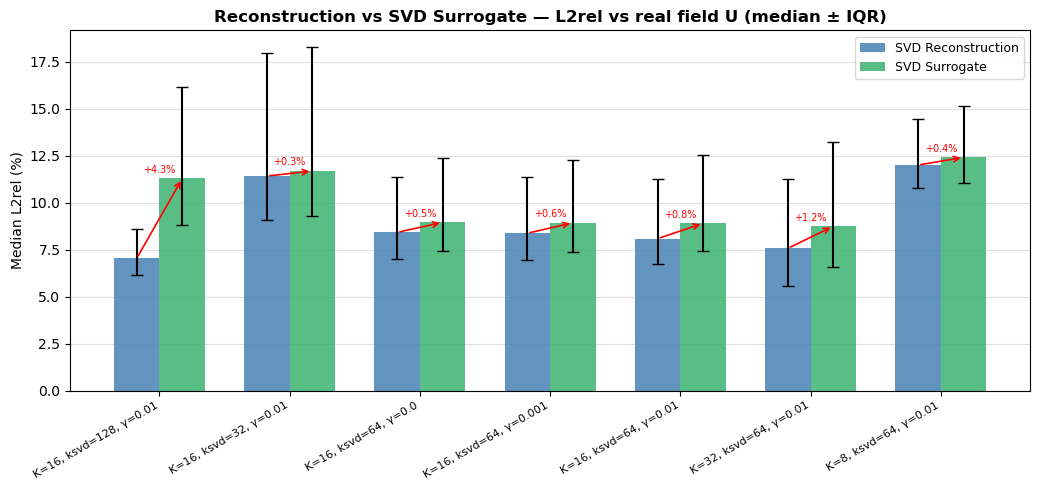
\includegraphics[width=\textwidth]{svd_rec_vs_surr.png}
    \caption{POD reconstruction (blue) vs.\ end-to-end surrogate (green): median relative $L^2$ error for all configurations (median $\pm$ IQR). Arrows indicate the surrogate overhead.}
    \label{fig:pod_rec_vs_surr}
\end{figure}

\paragraph{Linear reconstruction floor.}
The POD reconstruction error is governed by the singular value decay of the Laplace-domain field matrices $\bm{U}^{(k)}$: the linear basis is accurate at low Laplace frequencies, where the spatial mode structure is smooth and low-rank, but degrades steadily at higher frequencies where the fields become localized and the singular values decay more slowly. Increasing $k_{\mathrm{pod}}$ beyond 64 reduces this high-frequency error only marginally, indicating that the residual is not a truncation artifact but an intrinsic limit of the linear subspace; likewise, beyond $K=16$ the dominant transient content is already captured and additional frequencies add noise rather than information. The damping $\gamma$ is benign at the level of the global physical-field error (8.42\%, 8.38\%, 8.09\% for $\gamma = 0$, $0.001$, $0.01$), because two error sources cancel: a purely imaginary contour concentrates energy more tightly and lowers the POD truncation error at every frequency, while a larger $\gamma$ conversely damps the Tikhonov inversion error that propagates those residuals back to the time domain. Full ablations, including the per-frequency breakdown that exposes this trade-off, are given in Appendix~\ref{app:pod_ablation}.

\paragraph{Surrogate overhead.}
For most configurations the surrogate step adds little above the linear floor: the gap ranges from $+0.27$ pp ($k_{\mathrm{pod}}=32$) to $+1.17$ pp ($K=32$), confirming that the MLP predicts the POD coefficients from $\vmu$ reliably. The exception is $k_{\mathrm{pod}}=128$, $K=16$: despite the best reconstruction floor (7.04\%), the surrogate error rises to 11.29\% (gap $+4.26$ pp). With $2 \times K \times k_{\mathrm{pod}} = 4{,}096$ scalar targets, the higher-dimensional regression problem overwhelms the benefit of the larger basis. The best POD surrogate is therefore $k_{\mathrm{pod}}=64$, $K=16$, $\gamma=0.01$ (8.91\% median), the balance point between basis expressivity and surrogate learnability. Inference is fast throughout — 2.9\,ms ($K=8$) to 5.6\,ms ($K=32$) per sample at batch size 1, reaching 800--870 samples/s at batch size 32 — with the cost dominated by the back-projection through $\bm{V}^{(k)}$ and the Tikhonov inversion rather than the network forward pass.

This establishes the linear POD as a well-characterized reference: its error floor, set by the discarded singular values of $\bm{U}^{(k)}$, is the target that the non-linear autoencoders of Section~\ref{sec:ae_perf} are designed to push below. Per-sample error distributions for all configurations are provided in Appendix~\ref{app:histograms}.

\subsection{Autoencoder Performance}
\label{sec:ae_perf}

Table~\ref{tab:ae_results} reports the relative $L^2$ reconstruction error on the held-out test set (1620 simulations) for all trained AE checkpoints, evaluated on the physical field $U(t)$.

\begin{table}[htbp]
    \centering
    \small
    \setlength{\tabcolsep}{5pt}
    \renewcommand{\arraystretch}{1.3}
    \begin{tabular}{llcccrrrr}
        \toprule
        \textbf{Model} & $d_z$ & $K$ & $\gamma$ & \textbf{Median (\%)} & \textbf{Mean (\%)} & \textbf{p90 (\%)} & \textbf{vs.\ SVD (pp)} \\
        \midrule
        \multirow{7}{*}{LLAE}
          & 128 & 16 & 0.01  & \textbf{2.92} & 3.15 & 4.38  & $-4.12$ \\
          & 64  & 32 & 0.01  & 3.19 & 3.53 & 5.11  & $-4.38$ \\
          & 64  & 16 & 0.01  & 3.20 & 3.47 & 5.04  & $-4.89$ \\
          & 64  & 16 & 0.0   & 3.26 & 3.61 & 5.24  & $-5.16$ \\
          & 64  & 16 & 0.001 & 3.32 & 3.65 & 5.16  & $-5.06$ \\
          & 64  &  8 & 0.01  & 3.35 & 3.66 & 5.26  & $-8.66$ \\
          & 32  & 16 & 0.01  & 3.43 & 3.85 & 5.60  & $-7.99$ \\
        \midrule
        \multirow{7}{*}{SLAE}
          & 64  & 16 & 0.0   & \textbf{7.78} &  8.11 &  9.91 & $-0.64$ \\
          & 64  & 16 & 0.001 & 7.82  &  8.27 & 10.36 & $-0.56$ \\
          & 128 & 16 & 0.01  & 7.98  &  8.40 & 10.45 & $+0.94$ \\
          & 64  & 32 & 0.01  & 8.34  &  9.27 & 13.43 & $+0.77$ \\
          & 64  & 16 & 0.01  & 8.92  &  9.53 & 12.55 & $+0.83$ \\
          & 32  & 16 & 0.01  & 10.76 & 11.14 & 14.76 & $-0.66$ \\
          & 64  &  8 & 0.01  & 12.26 & 12.74 & 15.40 & $+0.25$ \\
        \bottomrule
    \end{tabular}
    \caption{Relative $L^2$ reconstruction error on the test set (1620 simulations). The last column gives the difference in median error relative to the linear POD baseline at matching $(K, k_{\mathrm{pod}}=d_z, \gamma)$: negative values indicate improvement over POD, positive values indicate that POD outperforms the AE. Best per family in bold.}
    \label{tab:ae_results}
\end{table}

Figure~\ref{fig:ae_bar_all} summarises the reconstruction floor across all 14 checkpoints. The two families present a stark contrast. LLAE achieves a best median error of 2.92\% ($d_z=128$, $K=16$), a factor of four below the linear SVD baseline. SLAE yields errors in the range 7.78\%--12.26\%, broadly comparable to SVD: the \emph{vs.\ SVD} column of Table~\ref{tab:ae_results} hovers around zero, positive as often as negative. Taken as a pure compression stage, SLAE does not offer a meaningful gain over the linear reference. This may appear disappointing, but the picture changes substantially at the surrogate stage (Section~\ref{sec:surr_results}).

Two compounding factors explain this divergence (Sections~\ref{sec:slae}--\ref{sec:llae}). First, the input spaces differ: SLAE compresses high-dimensional complex frequency frames $\hat{U}(s_k)$, whereas LLAE encodes smoother physical frames — an intrinsically easier task. Second, the training objectives are asymmetric: LLAE's loss~\eqref{eq:llae_loss} includes a direct physical-time reconstruction term that provides dense temporal supervision, while SLAE deliberately omits it during Phase~1 (Section~\ref{sec:slae}) to preserve its computational advantage.

\begin{figure}[htbp]
    \centering
    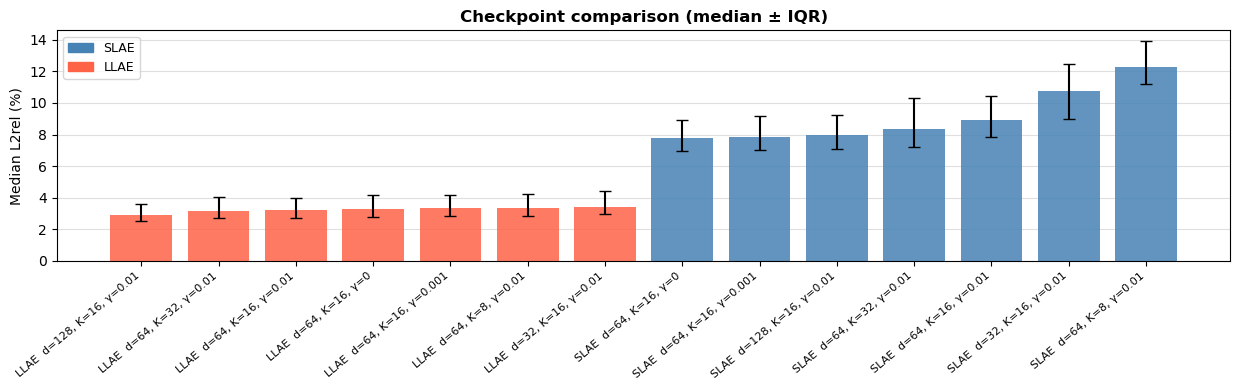
\includegraphics[width=\textwidth]{ae_bar_all.png}
    \caption{Reconstruction error for all 14 AE checkpoints, sorted by median relative $L^2$ error on the test set ($n=1620$, error bars = IQR). LLAE in red, SLAE in blue.}
    \label{fig:ae_bar_all}
\end{figure}

Figures~\ref{fig:llae_ablation} and~\ref{fig:slae_ablation} report ablation studies for each family, varying one hyperparameter at a time while holding the others fixed.

Within LLAE (Figure~\ref{fig:llae_ablation}), increasing the latent dimension from $d_z=32$ to $d_z=128$ reduces the median error from 3.43\% to 2.92\%, indicating that the latent bottleneck has not yet saturated at $d_z=64$. The number of Laplace frequencies $K$ has little impact: errors at $K=8$, 16, and 32 are 3.35\%, 3.20\%, and 3.19\% respectively, suggesting that 8–16 frequencies already capture the dominant transient dynamics. The damping parameter $\gamma$ is similarly insensitive in the range $[0, 0.01]$, consistent with the smooth energy envelope of the exponential decay at these timescales.

\begin{figure}[htbp]
    \centering
    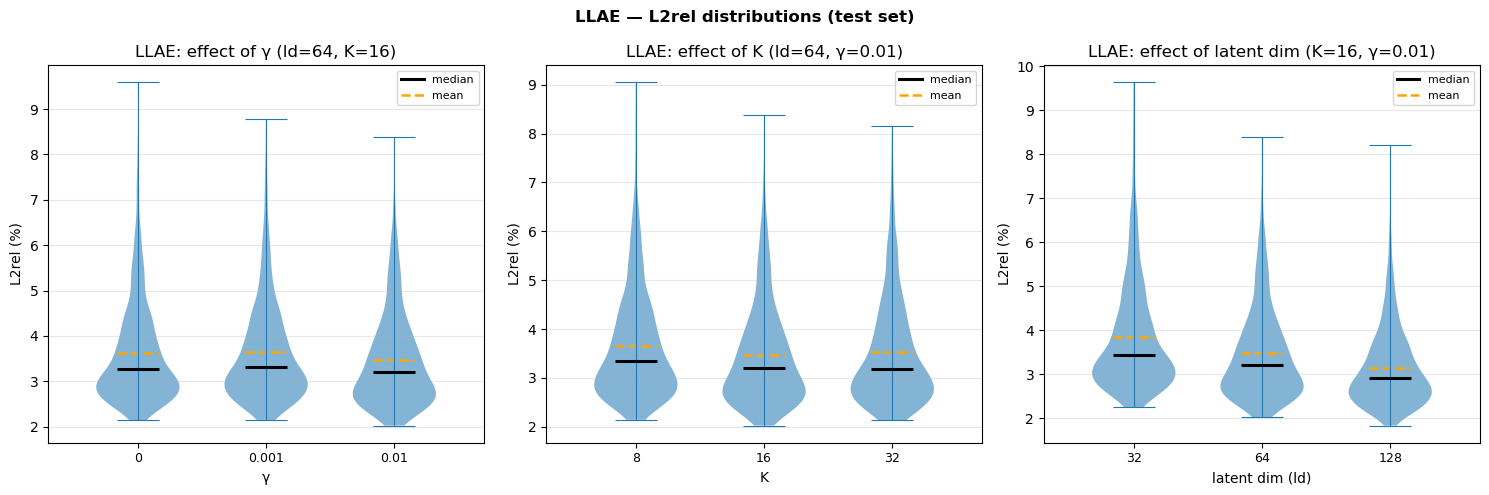
\includegraphics[width=\textwidth]{llae_ablation.png}
    \caption{LLAE ablation study. From left to right: effect of latent dimension $d_z$ ($K=16$, $\gamma=0.01$), number of Laplace frequencies $K$ ($d_z=64$, $\gamma=0.01$), and damping parameter $\gamma$ ($d_z=64$, $K=16$). Violin plots show the full error distribution; black line is the median, dashed orange line is the mean.}
    \label{fig:llae_ablation}
\end{figure}

Within SLAE (Figure~\ref{fig:slae_ablation}), errors increase sharply at low $K$ ($K=8$: 12.26\%) and low $d_z$ ($d_z=32$: 10.76\%), pointing to a harder compression problem where both the spectral and spatial bottlenecks are binding simultaneously. Increasing $K$ to 32 does not improve reconstruction (8.34\% vs.\ 7.78\% at $K=16$), likely because higher Laplace frequencies carry less spatial energy and expose the spatial compression bottleneck. The SLAE error distribution also shows a heavier right tail (higher p90) than LLAE, reflecting occasional failure cases where spatial compression degrades on outlier samples.

\begin{figure}[htbp]
    \centering
    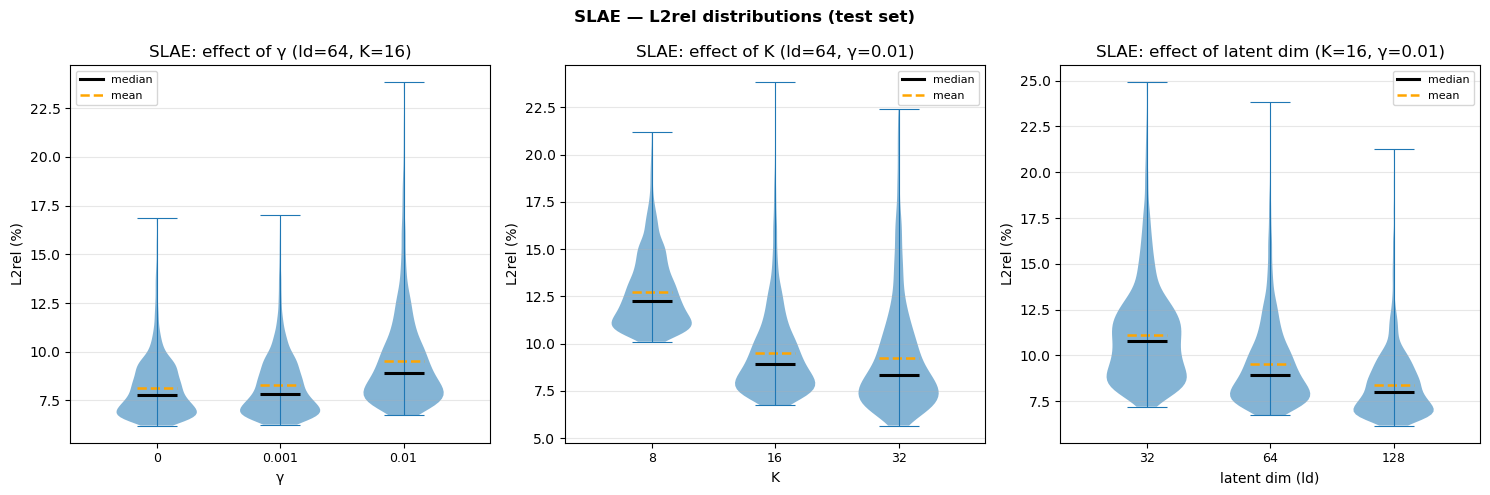
\includegraphics[width=\textwidth]{slae_ablation.png}
    \caption{SLAE ablation study. Same layout as Figure~\ref{fig:llae_ablation} (fixed parameters: $K=16$, $\gamma=0.01$ / $d_z=64$, $\gamma=0.01$ / $d_z=64$, $K=16$). Note the larger y-axis range compared to LLAE.}
    \label{fig:slae_ablation}
\end{figure}

For SLAE, Figure~\ref{fig:slae_per_freq} shows the reconstruction error broken down per Laplace frequency $k$. The error is lowest at low frequencies ($k=0$--3, where most signal energy is concentrated) and rises monotonically toward higher frequencies, confirming that the spatial compression bottleneck is more severe for the fine-scale, high-frequency content.

\begin{figure}[htbp]
    \centering
    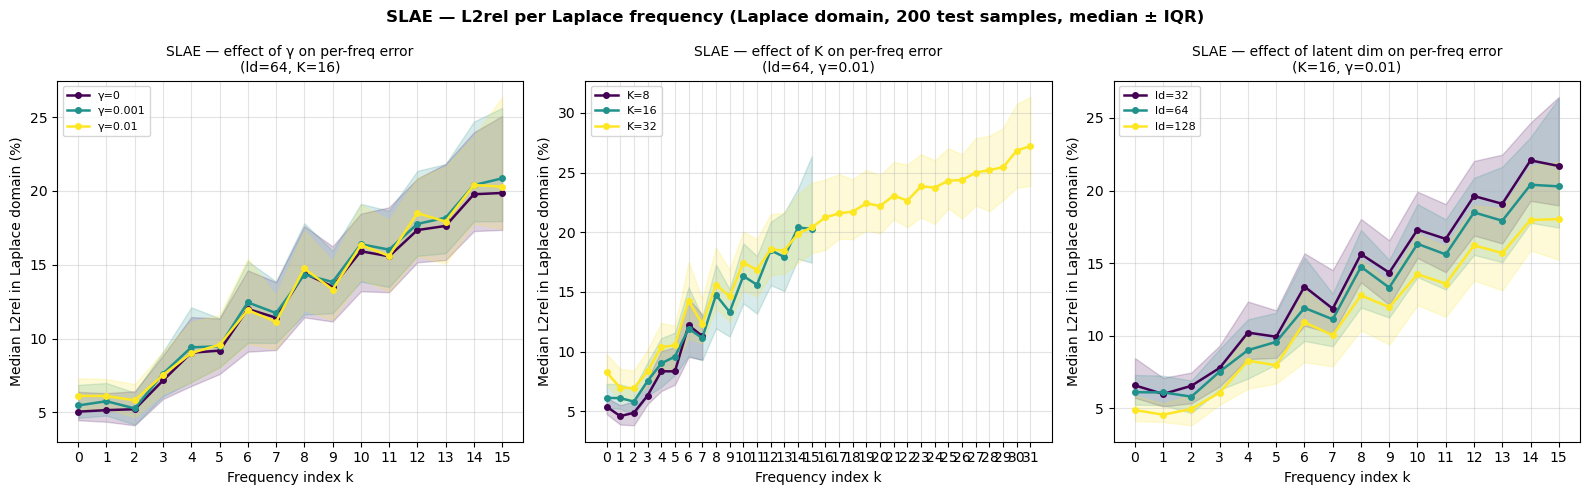
\includegraphics[width=\textwidth]{slae_per_freq.png}
    \caption{SLAE — per-frequency reconstruction error in the Laplace domain (median $\pm$ IQR, 200 test samples). Left: effect of $\gamma$; centre: effect of $K$; right: effect of $d_z$.}
    \label{fig:slae_per_freq}
\end{figure}

Comparing with the POD per-frequency breakdown (Figure~\ref{fig:pod_per_freq}), SLAE achieves roughly half the per-frequency error of POD at each $k$: the convolutional encoder captures non-linear structure that the linear projection cannot. Yet this per-frequency advantage does not translate into a better overall spatial reconstruction (Table~\ref{tab:ae_results}). The reason is Tikhonov regularisation: the inverse transform~\eqref{eq:tikhonov}--\eqref{eq:normal} damps all frequencies uniformly, so the benefit of encoding each frequency more accurately is partially cancelled before the spatial field is recovered. The global spatial error is therefore a \emph{regularisation-weighted} aggregate of the per-frequency errors, not a direct reflection of per-frequency compression quality.

\paragraph{Inference latency.}
Table~\ref{tab:bench} and Figure~\ref{fig:bench} report per-sample inference latency and GPU throughput measured with CUDA Events on an NVIDIA RTX 3090 (10 warm-up runs, 50 timed runs, batch size 1 for latency; max batch size for throughput). SLAE is approximately $2.4\times$ faster per sample than LLAE at $K=16$ (8.0\,ms vs.\ $\sim\!19$–20\,ms), a direct consequence of the architectural difference detailed in Sections~\ref{sec:slae}--\ref{sec:llae}: SLAE decodes only $K$ frequency frames at inference, whereas LLAE must decode all $N_t=150$ time frames. At $K=8$, SLAE latency drops to 5.5\,ms. SLAE also requires far less GPU memory (112\,MB at $K=16$ vs.\ 525\,MB for LLAE), enabling a $5\times$ larger maximum batch size.

\begin{table}[htbp]
    \centering
    \renewcommand{\arraystretch}{1.3}
    \begin{tabular}{lccrrr}
        \toprule
        \textbf{Model} & $K$ & $d_z$ & \textbf{Latency (ms)} & \textbf{Throughput (s/s)} & \textbf{Peak GPU (MB)} \\
        \midrule
        SLAE & 8  & 64  & $5.5 \pm 0.2$  & 224 & 56  \\
        SLAE & 16 & 64  & $8.0 \pm 0.1$  & 134 & 112 \\
        SLAE & 16 & 128 & $8.1 \pm 0.1$  & 133 & 112 \\
        SLAE & 32 & 64  & $13.9 \pm 0.4$ &  74 & 224 \\
        \midrule
        LLAE & 16 & 32  & $19.0 \pm 1.1$ &  56 & 525 \\
        LLAE & 16 & 64  & $19.4$--$20.1$ & 52--54 & 525 \\
        LLAE & 16 & 128 & $19.0 \pm 0.8$ &  56 & 525 \\
        \bottomrule
    \end{tabular}
    \caption{Inference benchmark on an NVIDIA RTX 3090. Latency: batch size 1, 50 timed CUDA Event runs after 10 warm-up runs. Throughput at maximum GPU-filling batch size.}
    \label{tab:bench}
\end{table}

\begin{figure}[htbp]
    \centering
    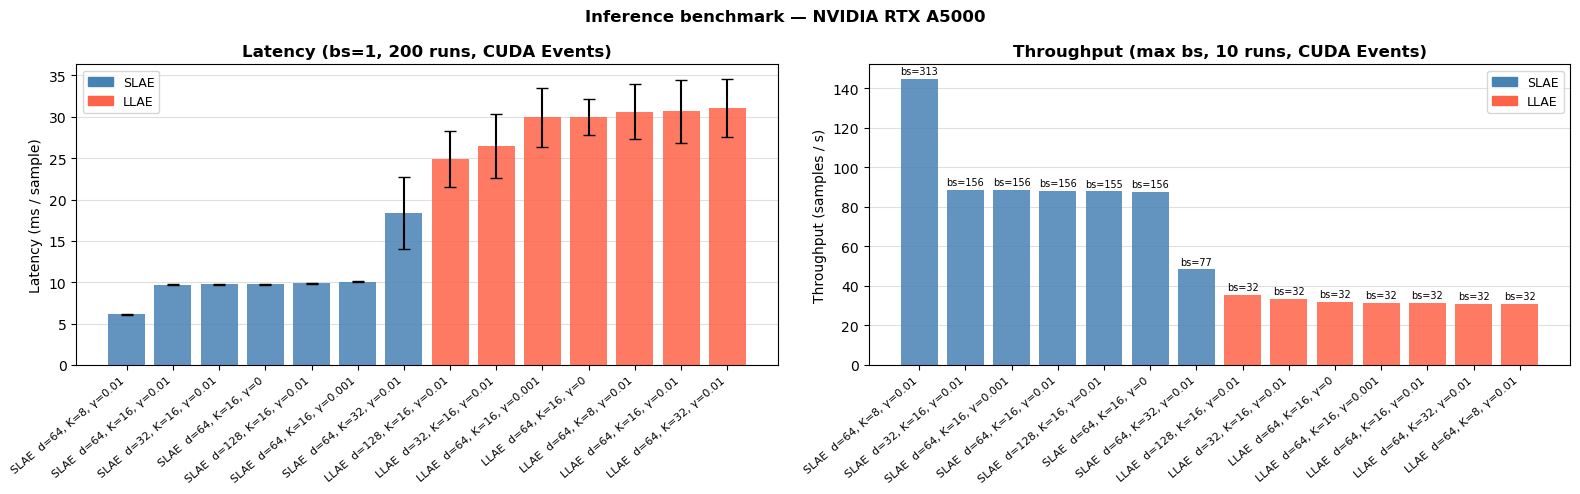
\includegraphics[width=\textwidth]{ae_inference_bench.png}
    \caption{Inference benchmark on an NVIDIA RTX 3090. Left: per-sample latency (batch size 1, 50 CUDA Event runs). Right: throughput at maximum GPU-filling batch size.}
    \label{fig:bench}
\end{figure}

\subsection{Surrogate Prediction Performance}
\label{sec:surr_results}

\subsubsection{Direct surrogate performance}
\label{sec:direct_surr}

Table~\ref{tab:surr_results} reports the relative $L^2$ error on the held-out test set (1620 simulations) for all 14 end-to-end surrogate checkpoints, evaluated on the physical field $U(t)$. All three model families (SVD, SLAE, LLAE) use the same surrogate MLP architecture (Appendix~\ref{app:architecture}), so the comparison isolates the effect of the spatial compression strategy rather than differences in the predictor capacity. Two additional columns facilitate interpretation: \emph{Gap} is the difference between the surrogate median and the standalone AE reconstruction median from Table~\ref{tab:ae_results} — a positive value indicates overhead introduced by the surrogate step, while a negative value means that joint fine-tuning of the decoder actually \emph{improves} upon the frozen-AE baseline; \emph{vs SVD} is the difference relative to the matching SVD surrogate from Table~\ref{tab:pod_surr_results} at the same $(K, d_z, \gamma)$, and is negative throughout, confirming that all AE surrogates outperform the linear baseline.

\begin{table}[htbp]
    \centering
    \small
    \setlength{\tabcolsep}{5pt}
    \renewcommand{\arraystretch}{1.3}
    \begin{tabular}{llcccrrrrr}
        \toprule
        \textbf{Model} & $d_z$ & $K$ & $\gamma$
            & \textbf{Median (\%)} & \textbf{Mean (\%)} & \textbf{p90 (\%)}
            & \textbf{Gap (pp)} & \textbf{vs POD (pp)} \\
        \midrule
        \multirow{7}{*}{LLAE}
          & 128 & 16 & 0.01  & \textbf{4.13} & 4.48 & 6.82  & $+1.21$ & $-7.16$ \\
          & 64  & 32 & 0.01  &          4.63 & 4.97 & 7.45  & $+1.44$ & $-4.12$ \\
          & 64  & 16 & 0.01  &          4.18 & 4.52 & 6.84  & $+0.98$ & $-4.73$ \\
          & 64  & 16 & 0.0   &          4.25 & 4.60 & 7.09  & $+0.99$ & $-4.71$ \\
          & 64  & 16 & 0.001 &          4.21 & 4.53 & 6.91  & $+0.89$ & $-4.73$ \\
          & 64  &  8 & 0.01  &          4.18 & 4.62 & 7.11  & $+0.83$ & $-8.23$ \\
          & 32  & 16 & 0.01  &          4.31 & 4.75 & 7.27  & $+0.88$ & $-7.38$ \\
        \midrule
        \multirow{7}{*}{SLAE}
          & 64  & 16 & 0.0   &          7.38 & 7.52 & 8.80  & $-0.40$ & $-1.58$ \\
          & 64  & 16 & 0.001 &          7.42 & 7.56 & 8.89  & $-0.40$ & $-1.52$ \\
          & 128 & 16 & 0.01  &          7.49 & 7.66 & 9.16  & $-0.49$ & $-3.80$ \\
          & 64  & 32 & 0.01  & \textbf{5.69} & 6.06 & 7.97  & $-2.65$ & $-3.06$ \\
          & 64  & 16 & 0.01  &          7.59 & 7.86 & 9.49  & $-1.33$ & $-1.32$ \\
          & 32  & 16 & 0.01  &          7.62 & 7.84 & 9.49  & $-3.14$ & $-4.07$ \\
          & 64  &  8 & 0.01  &         11.61 & 11.87 & 13.83 & $-0.65$ & $-0.80$ \\
        \bottomrule
    \end{tabular}
    \caption{Direct surrogate results on the test set (1620 simulations), same row order as Table~\ref{tab:ae_results}. \emph{Gap}: surrogate median $-$ AE reconstruction median; negative values indicate that end-to-end fine-tuning improves upon the standalone AE. \emph{vs POD}: surrogate median $-$ matching POD surrogate median (Table~\ref{tab:pod_surr_results}); all values are negative. Best per family in bold.}
    \label{tab:surr_results}
\end{table}

\paragraph{Overall accuracy.}
LLAE achieves 4.13--4.63\% median $L^2$ error across all configurations, compared to 5.69--11.61\% for SLAE. The best LLAE surrogate ($d_z=128$, $K=16$, $\gamma=0.01$, 4.13\%) represents a $\mathbf{54\%}$ reduction in median error relative to the best POD surrogate (8.91\%), while the best SLAE surrogate ($d_z=64$, $K=32$, $\gamma=0.01$, 5.69\%) achieves a $\mathbf{36\%}$ reduction. Figure~\ref{fig:surr_bar} summarises all 14 checkpoints sorted by median error.

\begin{figure}[htbp]
    \centering
    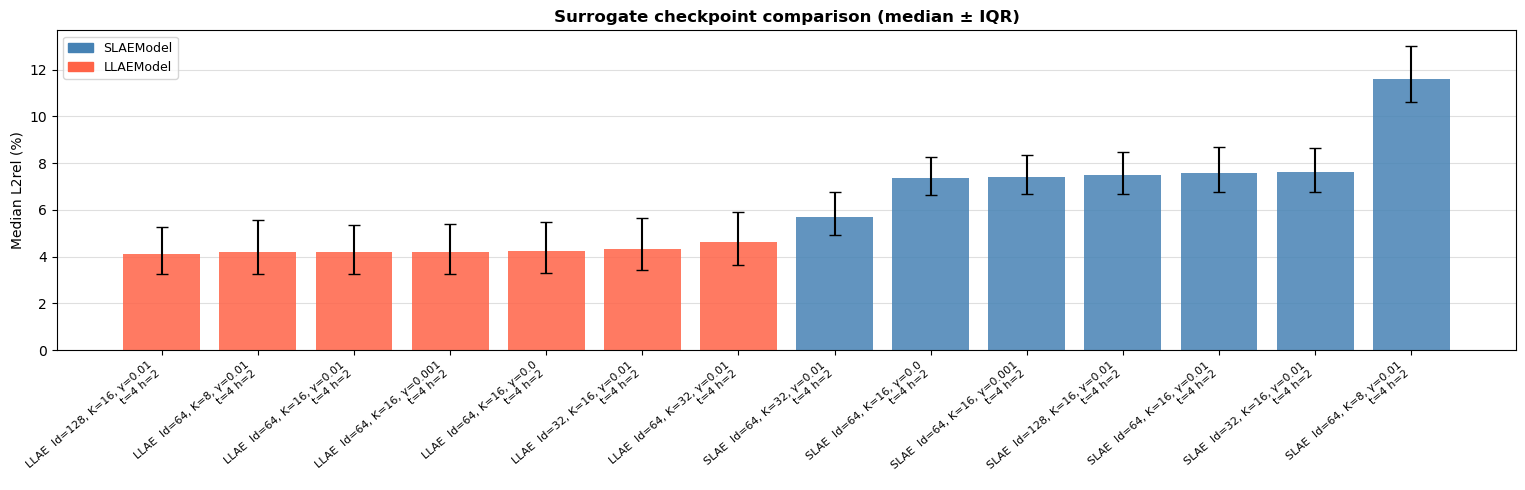
\includegraphics[width=\textwidth]{surr_bar.png}
    \caption{Surrogate checkpoint comparison: median $L^2$ relative error on the test set ($n=1620$), sorted by median with IQR error bars. LLAE (red) achieves 4.1--4.6\%, SLAE (blue) 5.7--11.6\%. The best POD surrogate (8.91\%) is indicated by a dashed horizontal line for reference.}
    \label{fig:surr_bar}
\end{figure}

\paragraph{End-to-end fine-tuning effect.}
The Gap column reveals a qualitative asymmetry between the two families. For LLAE, the surrogate step introduces a small positive overhead of $+0.83$ to $+1.44$\,pp above the AE reconstruction floor: the surrogate approximation is not perfectly lossless, but the cost is modest given that the AE floor itself already saturates below 3.5\%.

For SLAE, by contrast, the Gap is \emph{negative} across all configurations, ranging from $-0.40$ to $-3.14$\,pp — meaning that the end-to-end surrogate pipeline \emph{outperforms} the standalone SLAE autoencoder. The mechanism is the following. During Phase~1 (AE training), the SLAE loss $\mathcal{L}_{\mathrm{SLAE}}$ (equation~\eqref{eq:slae_loss}, Section~\ref{sec:slae}) is defined purely in the Laplace domain: the decoder is never directly supervised on physical-time reconstruction quality, as computing a physical-time loss would require $N_t$-frame decoder passes and negate SLAE's speed advantage. During Phase~2 (surrogate training), the combined loss $\mathcal{L}_{\mathrm{total}}$ (Section~\ref{sec:surrogate}) introduces a direct physical-time reconstruction term for the first time, and the decoder is jointly fine-tuned through it. This spatial supervision signal corrects residual errors that the Laplace-domain loss alone was unable to resolve. The effect is largest when the AE floor is highest: at $d_z=32$ ($-3.14$\,pp) and $K=32$ ($-2.65$\,pp), the spatial loss during surrogate training compensates for the harder compression task, lowering the error below the standalone AE baseline.

\paragraph{Hyperparameter sensitivity.}
LLAE surrogates remain highly robust: varying $K$ from 8 to 32, $d_z$ from 32 to 128, or $\gamma$ from 0 to 0.01 all yield errors in a tight 4.13--4.63\% band, consistent with the insensitivity already observed at the AE level (Section~\ref{sec:ae_perf}). SLAE is more sensitive: $K=8$ collapses to 11.61\% (the spectral truncation is too severe for the surrogate to compensate), while $K=32$ is the best SLAE configuration precisely because the decoder, given access to 32 Laplace frequencies, can recover finer spatial structure during fine-tuning. Ablation violin plots are provided in Appendix~\ref{app:surr_ablation}.

\paragraph{Inference latency.}
The surrogate MLP (architecture detailed in Appendix~\ref{app:architecture}) adds negligible latency to the AE decoding pipeline: measured on an NVIDIA RTX A5000, SLAE at $K=16$ runs at $8.4 \pm 0.1$\,ms per sample and LLAE at $18.3 \pm 0.7$\,ms, virtually identical to the AE-only figures reported in Table~\ref{tab:bench} and consistent with the linear projection cost dominating over the network forward pass. SLAE therefore preserves its ${\approx}2.2\times$ latency advantage over LLAE. Figure~\ref{fig:surr_bench} details the latency breakdown across all 14 checkpoints.

\begin{figure}[htbp]
    \centering
    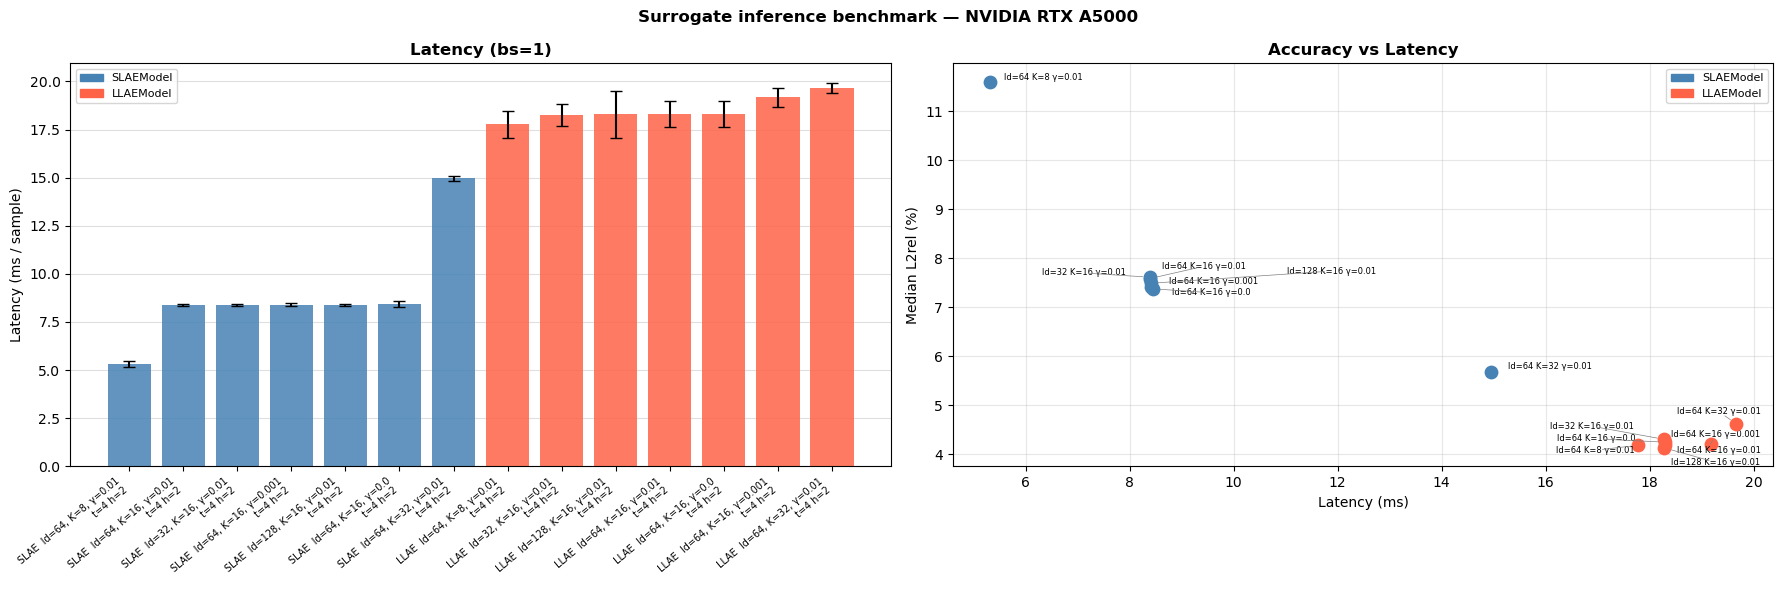
\includegraphics[width=\textwidth]{surr_bench.png}
    \caption{Surrogate inference benchmark (NVIDIA RTX A5000, 50 CUDA Event timed runs, batch size 1). Left: per-sample latency by model family and $K$. Right: accuracy--latency scatter (median $L^2$ error vs.\ latency).}
    \label{fig:surr_bench}
\end{figure}

Per-checkpoint error histograms for all 14 surrogate checkpoints are provided in Appendix~\ref{app:histograms} (Figure~\ref{fig:surr_histograms}).

\subsubsection{SVD surrogates: single-mode latent compression}
\label{sec:ae_svd_surr}

The direct surrogate of Section~\ref{sec:direct_surr} predicts the full $d_z$-dimensional latent at each frequency. To evaluate whether compressing that representation before learning the dynamics can instead improve the predictor's accuracy, we assess a hybrid approach inspired by Rank Reduction Autoencoders (RRAE) \cite{mounayer2025}: projecting the latent trajectories onto a truncated SVD basis before applying the surrogate model. We evaluate 26 AE+SVD surrogate checkpoints across the LLAE and SLAE families. In these models the encoder is frozen, whereas the decoder and the SVD basis $V$ are trained end-to-end alongside the surrogate; the latent dimension is reduced to $k_{\mathrm{svd}}$ (either 16 or 32) via POD (SVD) before an MLP predicts the reduced coefficients from the physical parameters. 

Table~\ref{tab:ae_svd_surr_results} reports the relative $L^2$ error on the held-out test set evaluated on the physical field $U(t)$.

\begin{table}[htbp]
    \centering
    \small
    \setlength{\tabcolsep}{5pt}
    \renewcommand{\arraystretch}{1.3}
    \begin{tabular}{llcccrrrr}
        \toprule
        \textbf{Model} & $d_z$ & $K$ & $\gamma$ & $k_{\mathrm{svd}}$
            & \textbf{Median (\%)} & \textbf{Mean (\%)} & \textbf{p90 (\%)} \\
        \midrule
        \multirow{14}{*}{LLAE}
          & 64  & 16 & 0.01  & 32 & \textbf{4.24} & 4.61 & 6.75 \\
          & 64  & 32 & 0.01  & 32 & 4.29 & 4.69 & 7.02 \\
          & 64  & 16 & 0.001 & 32 & 4.44 & 4.96 & 7.41 \\
          & 64  & 16 & 0.0   & 32 & 4.50 & 4.97 & 7.29 \\
          & 64  &  8 & 0.01  & 32 & 4.60 & 5.04 & 7.47 \\
          & 128 & 16 & 0.01  & 32 & 4.77 & 5.30 & 7.82 \\
          & 32  & 16 & 0.01  & 16 & 5.55 & 6.29 & 9.39 \\
          & 64  & 32 & 0.01  & 16 & 5.58 & 6.22 & 9.35 \\
          & 128 & 16 & 0.01  & 16 & 5.83 & 6.51 & 9.48 \\
          & 64  & 16 & 0.01  & 16 & 5.84 & 6.58 & 9.79 \\
          & 64  & 16 & 0.001 & 16 & 5.90 & 6.72 & 9.92 \\
          & 64  & 16 & 0.0   & 16 & 5.94 & 6.76 & 10.18 \\
          & 64  &  8 & 0.01  & 16 & 6.54 & 7.37 & 11.05 \\
        \midrule
        \multirow{12}{*}{SLAE}
          & 64  & 32 & 0.01  & 32 & \textbf{6.03} & 6.58 & 9.02 \\
          & 64  & 32 & 0.01  & 16 & 6.96 & 7.80 & 11.24 \\
          & 64  & 16 & 0.0   & 32 & 7.50 & 7.73 & 9.26 \\
          & 64  & 16 & 0.001 & 32 & 7.62 & 7.88 & 9.52 \\
          & 64  & 16 & 0.01  & 32 & 7.90 & 8.32 & 10.54 \\
          & 32  & 16 & 0.01  & 16 & 7.95 & 8.38 & 10.71 \\
          & 64  & 16 & 0.001 & 16 & 8.01 & 8.43 & 10.80 \\
          & 128 & 16 & 0.01  & 32 & 8.12 & 8.57 & 10.98 \\
          & 64  & 16 & 0.0   & 16 & 8.13 & 8.61 & 11.06 \\
          & 64  & 16 & 0.01  & 16 & 8.71 & 9.40 & 12.68 \\
          & 128 & 16 & 0.01  & 16 & 8.89 & 9.71 & 13.43 \\
          & 64  &  8 & 0.01  & 32 & 11.64 & 11.93 & 13.96 \\
          & 64  &  8 & 0.01  & 16 & 11.97 & 12.38 & 14.88 \\
        \bottomrule
    \end{tabular}
    \caption{AE+SVD surrogate results on the test set ($n=1620$), evaluating the physical field reconstruction error using LLAE and SLAE autoencoders coupled with an intermediate SVD compression ($k_{\mathrm{svd}} \in \{16, 32\}$). Best median per family in bold.}
    \label{tab:ae_svd_surr_results}
\end{table}

\paragraph{Does compressing the latent space help?}
The central question is whether predicting on a smaller, orthogonalised latent space simplifies the MLP's task enough to offset the information lost to SVD truncation. It does not. Measured \emph{at matching autoencoder configuration}, the SVD bottleneck adds a small penalty over the direct surrogate for both families: fixing $d_z=64$, $\gamma=0.01$, the best LLAE-SVD ($K=16$, $k_{\mathrm{svd}}=32$, 4.24\%) sits $+0.06$\,pp above its direct counterpart (4.18\%), and the best SLAE-SVD ($K=32$, $k_{\mathrm{svd}}=32$, 6.03\%) $+0.34$\,pp above its own (5.69\%). The MLP navigates the full $d_z$-dimensional latent space perfectly well, so the SVD projection merely discards spatial detail the direct surrogate had already learned to predict — compressing the latent before the surrogate degrades the reconstruction rather than helping it. Figure~\ref{fig:svd_surr_medians} collects the per-checkpoint medians.

\begin{figure}[htbp]
    \centering
    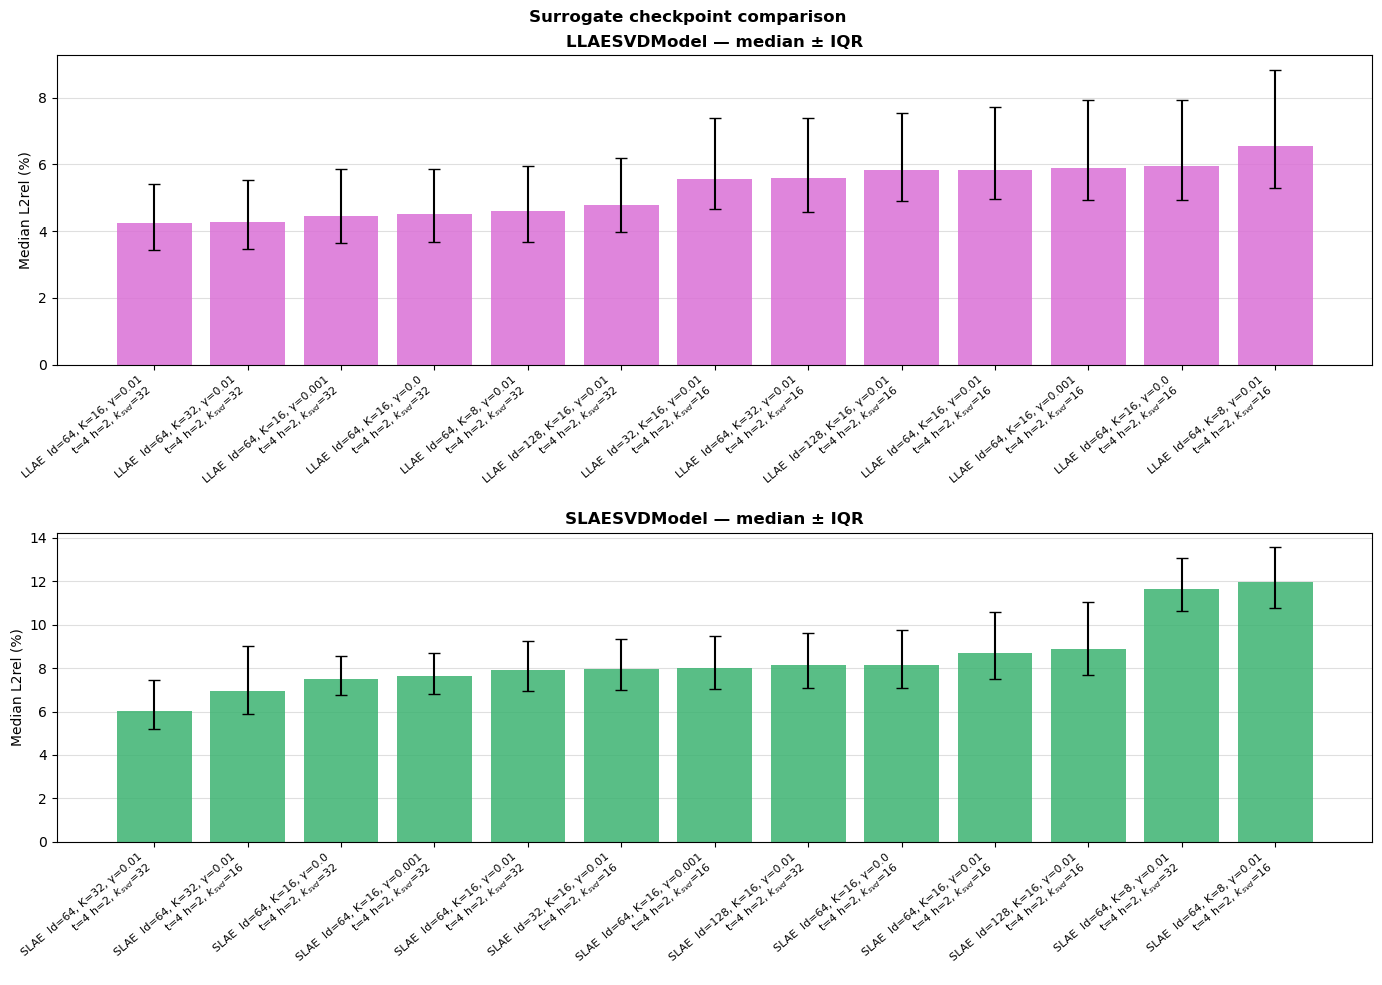
\includegraphics[width=0.8\textwidth]{svd_surr_medians.png}
    \caption{AE+SVD surrogate checkpoint comparison: median $L^2$ relative error with IQR error bars, grouping by model family. LLAE achieves 4.2--6.5\%, SLAE 6.0--12.0\%.}
    \label{fig:svd_surr_medians}
\end{figure}

\paragraph{Impact of $k_{\mathrm{svd}}$.}
To quantify the benefit of retaining a larger number of SVD modes, we compare pairs of configurations differing only in $k_{\mathrm{svd}}$ (16 vs.\ 32). Figure~\ref{fig:svd_surr_ksvd_impact} highlights that setting $k_{\mathrm{svd}}=32$ systematically improves the surrogate's accuracy across all models (all points lie below the $y=x$ diagonal). The gain is significantly more pronounced for LLAE models (between $+1.06$ and $+1.94$\,pp reduction in median error) than for SLAE models ($+0.33$ to $+0.93$\,pp), indicating that LLAE latent spaces contain more useful fine-grained information captured by the additional 16 SVD modes, whereas SLAE may inherently discard spatial details at the AE stage, limiting the potential gains of a larger $k_{\mathrm{svd}}$.

\begin{figure}[htbp]
    \centering
    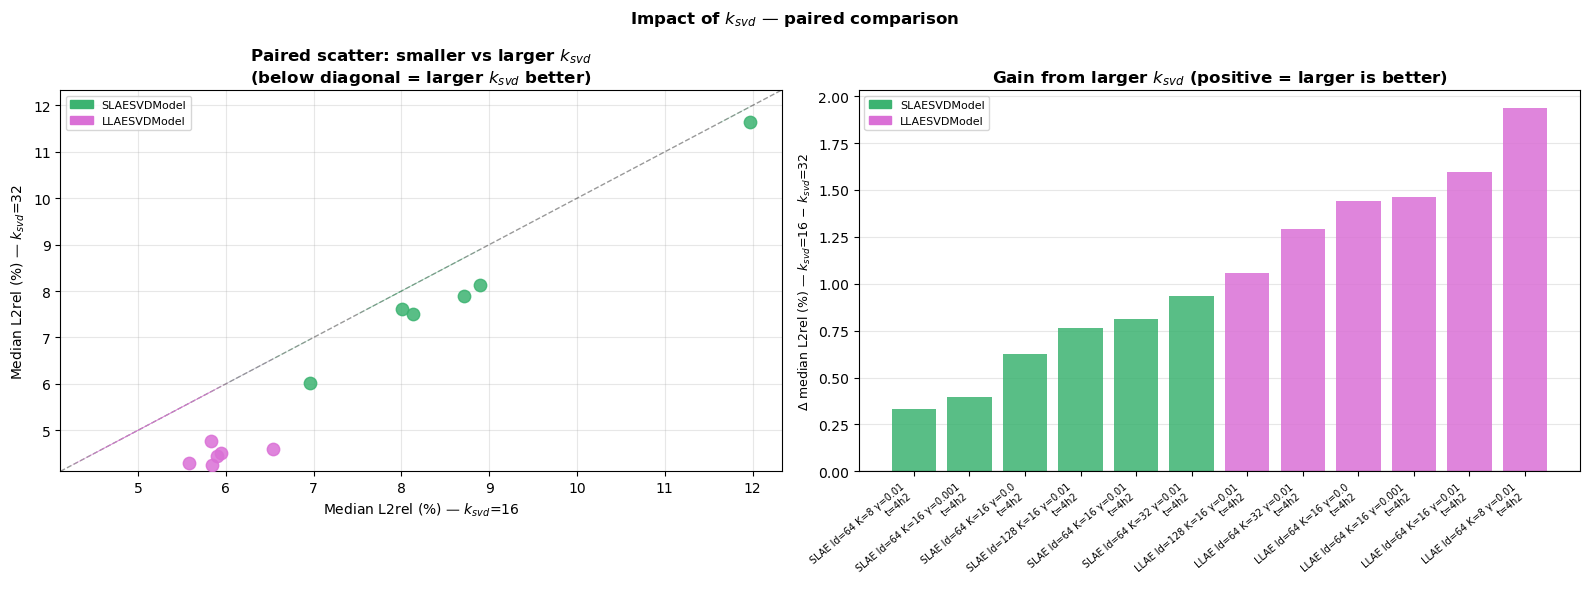
\includegraphics[width=\textwidth]{svd_surr_ksvd_impact.png}
    \caption{Impact of $k_{\mathrm{svd}}$ on SVD surrogate performance. Left: Scatter of paired median errors showing $k_{\mathrm{svd}}=32$ consistently outperforms $k_{\mathrm{svd}}=16$. Right: Absolute error reduction when shifting from 16 to 32 modes, sorted by magnitude.}
    \label{fig:svd_surr_ksvd_impact}
\end{figure}

\paragraph{Hyperparameter sensitivity.}
Sensitivity to the AE hyperparameters $K$, $d_z$, and $\gamma$ mirrors the direct case (Section~\ref{sec:direct_surr}): SLAE again degrades sharply at $K=8$ (11.6--12.0\%), while LLAE stays within a tight band. The lever specific to this pipeline is $k_{\mathrm{svd}}$, whose effect is quantified above: retaining 32 rather than 16 modes is uniformly beneficial, and more so for LLAE than for SLAE.

\paragraph{Inference latency.}
Introducing the SVD decoding step (matrix multiplication) between the MLP prediction and the spatial decoder adds a slight computational overhead. Measured on an NVIDIA RTX A5000 (batch size 1), LLAE-SVD requires approximately 22\,ms per sample, while SLAE-SVD requires about 9\,ms per sample. The SLAE-SVD model maintains its pronounced speed advantage (${\approx}2.4\times$) over LLAE-SVD, reflecting its lighter decoder architecture. The trade-off between latency and median error for AE+SVD surrogates is presented in Figure~\ref{fig:svd_surr_latency}.

\begin{figure}[htbp]
    \centering
    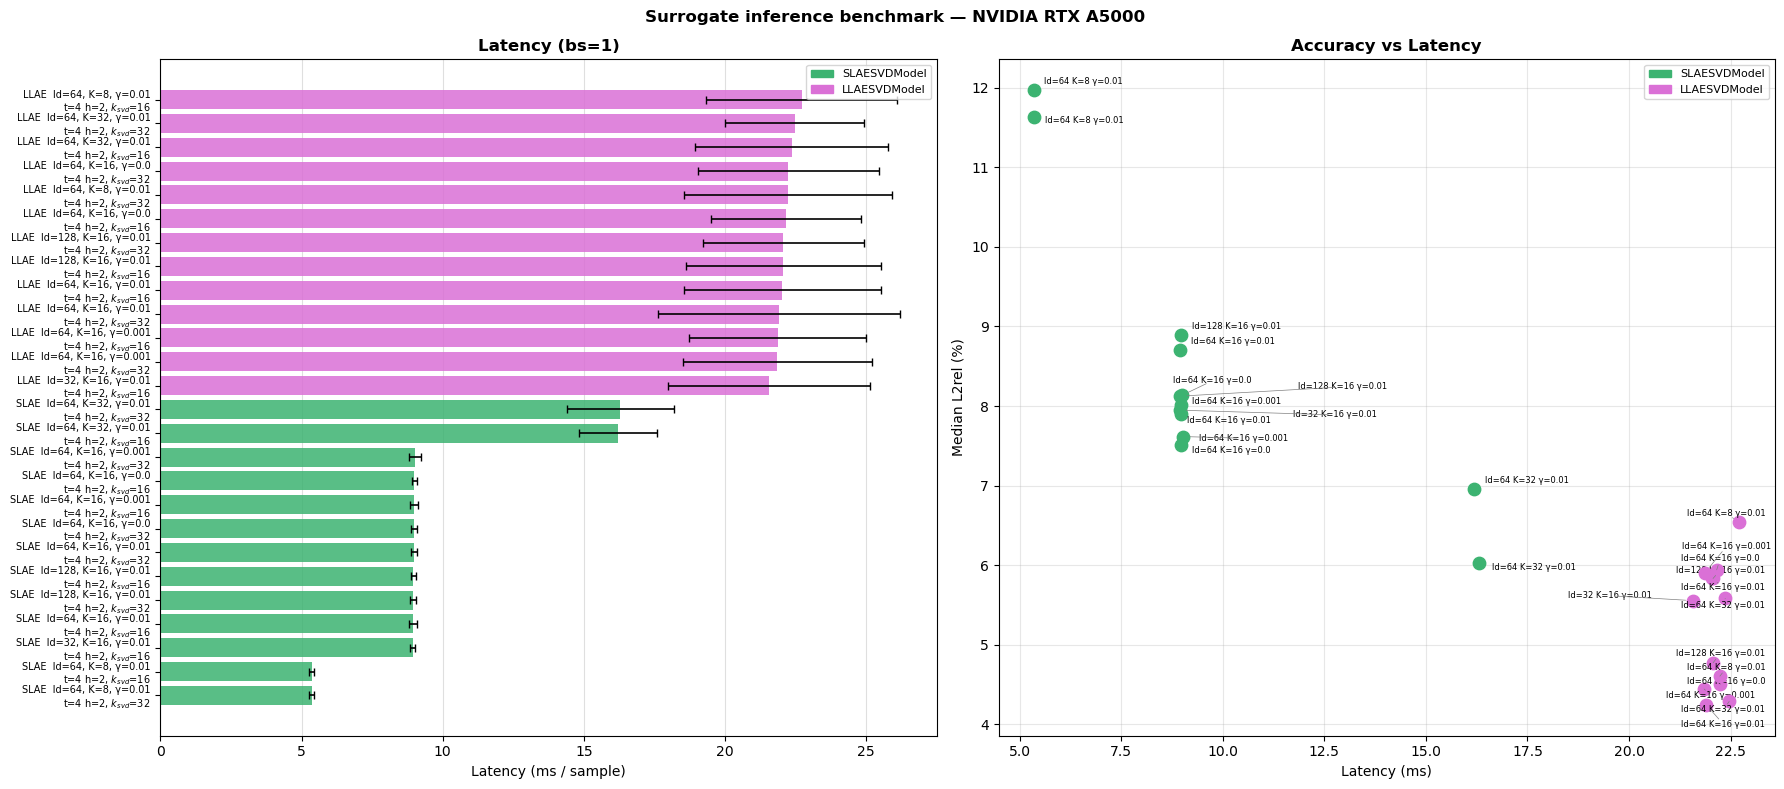
\includegraphics[width=\textwidth]{svd_surr_latency.png}
    \caption{AE+SVD surrogate inference benchmark (NVIDIA RTX A5000). Left: per-sample latency across checkpoints. Right: accuracy--latency scatter representing median $L^2$ error vs.\ latency.}
    \label{fig:svd_surr_latency}
\end{figure}
\subsubsection{Tucker surrogates: joint-mode latent compression}
\label{sec:tucker_surr}

Section~\ref{sec:ae_svd_surr} compressed the latent representation along a single mode. We now evaluate the Tucker variant of Section~\ref{sec:surrogate}, which factorises the frequency and latent modes \emph{jointly}: the surrogate predicts a compact core matrix $\hat{\mathcal{G}} \in \C^{r_s \times r_z}$ (real-valued for SLAE) instead of $K$ independent latents of dimension $d_z$, back-projecting through the frozen HOOI factors $U^{(s)}, U^{(z)}$ before decoding. We sweep the Tucker ranks over a grid $r_s \in \{4, 8\}$ (frequency mode, $K = 16 \to r_s$) $\times\ r_z \in \{8, 16, 32\}$ (latent mode, $d_z = 64 \to r_z$), for both families, yielding 12 checkpoints. All share the same Phase~1 autoencoder ($d_z = 64$, $K = 16$, $\gamma = 0.01$); only the offline factors and the surrogate differ. The compression ratio $\rho = r_s r_z / (K d_z)$ measures the reduction of the surrogate target dimension relative to the direct pipeline (which predicts $K d_z = 1024$ scalars per sample).

Beyond the physical-field error $\varepsilon_{\mathrm{field}}$ (relative $L^2$ on $U(t)$, full pipeline), we report two decoder-free diagnostics computed in the latent space, which split the difficulty between the offline compression and the surrogate MLP:
\begin{equation}
    \varepsilon_{\mathrm{trunc}} = \frac{\|\hat{Z} - \Pi\hat{Z}\|}{\|\hat{Z}\|},
    \qquad
    \varepsilon_{\mathrm{reg}} = \frac{\|\hat{\mathcal{G}}_{\mathrm{pred}} - \hat{\mathcal{G}}_{\mathrm{true}}\|}{\|\hat{\mathcal{G}}_{\mathrm{true}}\|},
\end{equation}
where $\Pi = U^{(s)}U^{(s)\top}(\cdot)\,U^{(z)}U^{(z)\top}$ is the Tucker projector. $\varepsilon_{\mathrm{trunc}}$ measures the energy discarded by the rank truncation (factors only, independent of the surrogate), while $\varepsilon_{\mathrm{reg}}$ measures how well the MLP predicts the true core (surrogate only, independent of the truncation). Table~\ref{tab:tucker_surr_results} reports all three on the held-out test set.

\begin{table}[htbp]
    \centering
    \small
    \setlength{\tabcolsep}{5pt}
    \renewcommand{\arraystretch}{1.3}
    \begin{tabular}{llccrrrrrr}
        \toprule
        \textbf{Model} & $r_s$ & $r_z$ & $\rho$
            & \textbf{Median (\%)} & \textbf{Mean (\%)} & \textbf{p90 (\%)}
            & $\varepsilon_{\mathrm{trunc}}$ (\%) & $\varepsilon_{\mathrm{reg}}$ (\%)
            & \textbf{Lat (ms)} \\
        \midrule
        \multirow{6}{*}{LLAE}
          & 8 & 32 & 0.250 & \textbf{4.33} & 4.75 &  7.16 & 36.98 & 7.25 & 18.2 \\
          & 4 & 32 & 0.125 &          4.57 & 5.04 &  7.61 & 40.34 & 5.67 & 18.0 \\
          & 8 & 16 & 0.125 &          4.87 & 5.43 &  8.11 & 61.86 & 4.38 & 18.3 \\
          & 4 & 16 & 0.062 &          5.16 & 5.77 &  8.70 & 61.59 & 3.83 & 18.0 \\
          & 8 &  8 & 0.062 &          6.85 & 7.78 & 11.75 & 81.21 & 4.99 & 18.3 \\
          & 4 &  8 & 0.031 &          6.87 & 8.02 & 12.73 & 81.03 & 3.80 & 18.0 \\
        \midrule
        \multirow{6}{*}{SLAE}
          & 8 & 32 & 0.250 & \textbf{7.92} & 8.35 & 10.55 & 42.40 & 6.76 & 7.4 \\
          & 4 & 32 & 0.125 &          8.15 & 8.68 & 11.14 & 50.82 & 6.58 & 7.1 \\
          & 4 & 16 & 0.062 &          8.68 & 9.36 & 12.79 & 69.59 & 5.18 & 7.1 \\
          & 8 & 16 & 0.125 &          8.85 & 9.51 & 12.89 & 67.59 & 5.83 & 7.5 \\
          & 4 &  8 & 0.031 &          9.93 & 10.92 & 15.61 & 80.63 & 5.70 & 7.1 \\
          & 8 &  8 & 0.062 &          9.96 & 11.05 & 16.00 & 80.05 & 7.16 & 7.5 \\
        \bottomrule
    \end{tabular}
    \caption{Tucker surrogate results on the test set ($n = 1620$), sorted by median error within each family. $\rho = r_s r_z / (K d_z)$ is the compression ratio of the surrogate target relative to the direct pipeline. $\varepsilon_{\mathrm{trunc}}$: median latent-energy discarded by the rank truncation (factors only). $\varepsilon_{\mathrm{reg}}$: median relative error of the predicted core (surrogate only). \emph{Lat}: GPU inference latency at batch size 1 (NVIDIA RTX A5000). Best median per family in bold.}
    \label{tab:tucker_surr_results}
\end{table}

\begin{figure}[htbp]
    \centering
    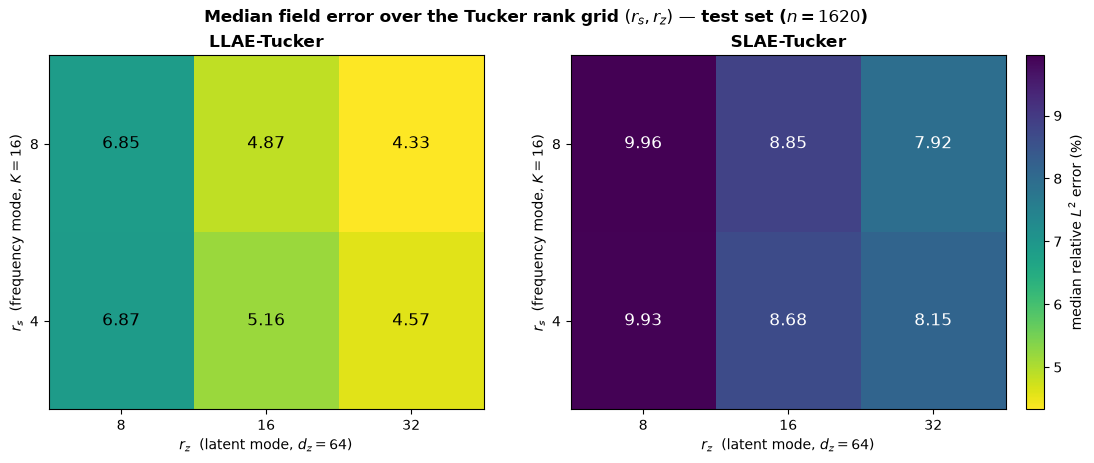
\includegraphics[width=\textwidth]{tucker_grid.png}
    \caption{Median field error over the Tucker rank grid $(r_s, r_z)$ (test set, $n = 1620$), for LLAE-Tucker (left) and SLAE-Tucker (right). Both panels share the same colour scale. The latent-mode rank $r_z$ (horizontal) drives the error far more than the frequency-mode rank $r_s$ (vertical).}
    \label{fig:tucker_grid}
\end{figure}

\paragraph{Overall accuracy.}
As with SVD, the relevant question is what the extra compression costs relative to the direct and single-mode pipelines \emph{at matching autoencoder configuration}. Fixing the shared AE ($d_z=64$, $K=16$, $\gamma=0.01$), the median error grows only gently along the compression axis: $4.18\% \to 4.24\% \to 4.33\%$ for LLAE (direct $\to$ SVD with $k_{\mathrm{svd}}=32$ $\to$ Tucker with $r_s=8$, $r_z=32$), and $7.59\% \to 7.90\% \to 7.92\%$ for SLAE. Tucker thus adds at most $+0.15$\,pp over the direct surrogate and $+0.09$\,pp over SVD — while shrinking the surrogate target to $r_s r_z = 256$ scalars, a $4\times$ reduction over the direct target ($K d_z = 1024$) and a $2\times$ reduction over the SVD target ($K k_{\mathrm{svd}} = 512$). Factorising both modes at once is what buys this: exploiting cross-frequency correlations lets Tucker match the single-mode SVD accuracy at half the target dimension.

\paragraph{Rank sensitivity: $r_z$ dominates $r_s$.}
The grid of Figure~\ref{fig:tucker_grid} is strongly anisotropic, and this is the most informative outcome of the sweep. Increasing the latent-mode rank $r_z$ from 8 to 32 nearly halves the LLAE error (6.85\% $\to$ 4.33\% at $r_s=8$), and the SLAE error falls in step (9.96\% $\to$ 7.92\%). Doubling the frequency-mode rank $r_s$ from 4 to 8, by contrast, barely moves either ($4.57\% \to 4.33\%$ for LLAE, $8.15\% \to 7.92\%$ for SLAE at $r_z=32$) — an effect an order of magnitude smaller. The rank sweeps of Figure~\ref{fig:tucker_rank_sweep} confirm the pattern distributionally: the $r_z$ violins separate cleanly while the $r_s$ violins overlap almost completely.

The interpretation reaches beyond this ablation. A rank-4 basis over the frequency mode already captures almost all of the joint variation of the $K=16$ Laplace coefficients across the training set: the spectral representation is redundant enough that discarding three quarters of its dimensions costs nothing measurable. The $d_z=64$ latent channels behave in the opposite way — they carry richer, less redundant information that a rank-8 basis truncates too aggressively. A tensor factorisation, fitted blind to the physics on training statistics alone, thus rediscovers the premise of this work: the Laplace representation is intrinsically compact along the frequency axis, and $K=16$ already sits close to its useful floor. That this evidence arrives from a direction independent of the argument which motivated the transform is what makes it worth reporting.

In practice $r_s=4$ is the parameter-efficient choice: it halves the surrogate size (1.35\,M vs.\ 1.9\,M parameters for $r_s=8$) at a negligible accuracy cost. One caveat bounds the claim: the frequency axis is sampled at two points only ($r_s \in \{4,8\}$), so the sweep establishes that the error is insensitive to $r_s$ over that range, not that it has saturated. The uncompressed limit $r_s = K$ is structurally the single-mode compression of Section~\ref{sec:ae_svd_surr}, although the two differ in the nature of the basis — real and trained there, complex and frozen here.

\begin{figure}[htbp]
    \centering
    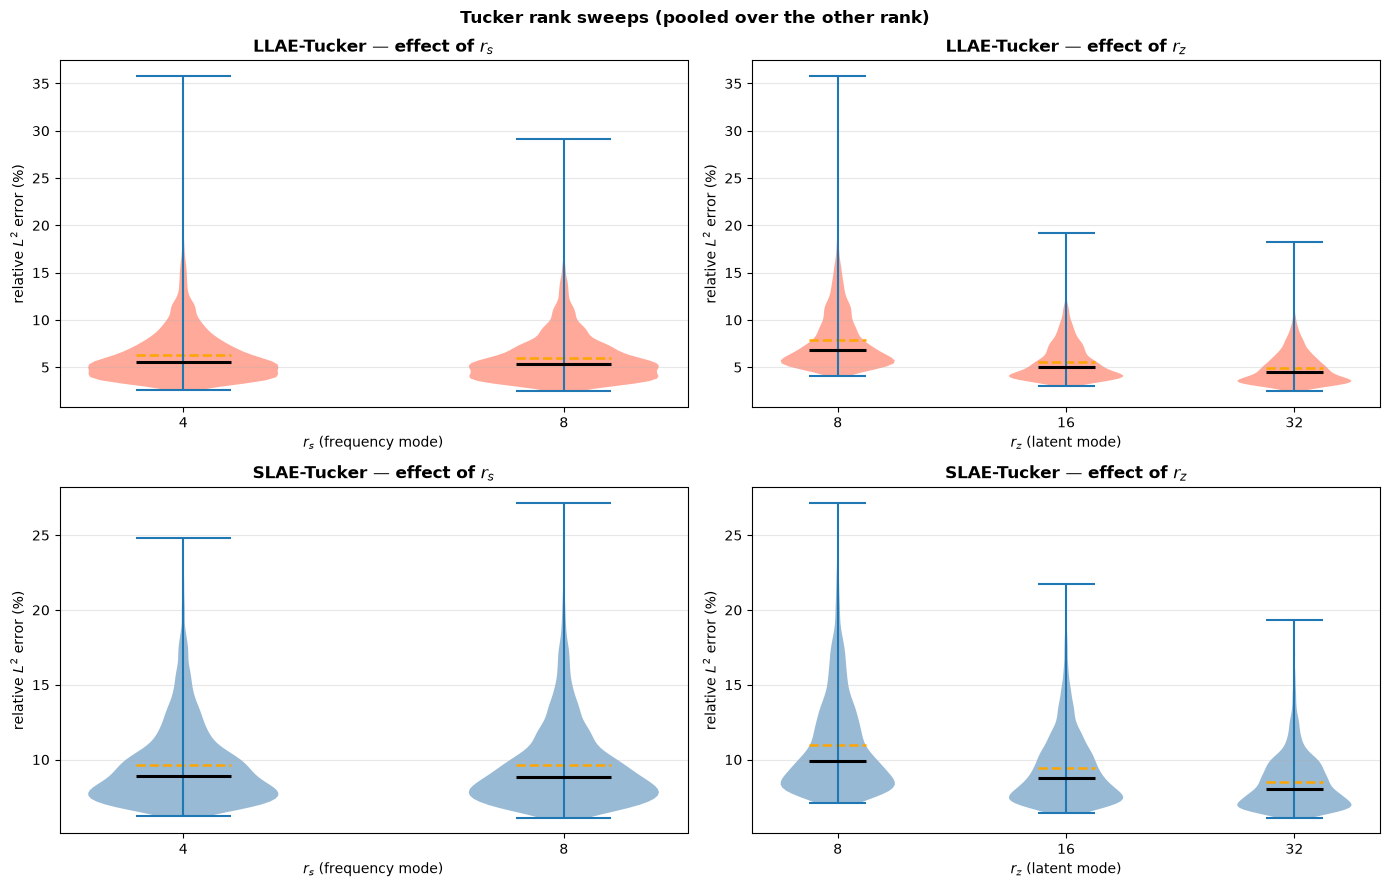
\includegraphics[width=\textwidth]{tucker_rank_sweep.png}
    \caption{Tucker rank sweeps (test set, violin plots pooled over the other rank; black line = median, dashed orange = mean). Top row LLAE-Tucker, bottom row SLAE-Tucker; left column effect of $r_s$, right column effect of $r_z$. The latent-mode rank $r_z$ separates the distributions, the frequency-mode rank $r_s$ does not.}
    \label{fig:tucker_rank_sweep}
\end{figure}

\paragraph{Truncation vs regression.}
The two decoder-free diagnostics of Table~\ref{tab:tucker_surr_results}, shown in Figure~\ref{fig:tucker_error_decomp}, locate the accuracy bottleneck. The regression error $\varepsilon_{\mathrm{reg}}$ stays small throughout (3.8--7.3\%): the MLP predicts the compact core reliably, and it grows only mildly as the core enlarges ($r_z=32$ is harder to fit than $r_z=8$). The truncation error $\varepsilon_{\mathrm{trunc}}$, by contrast, is large and is what the field error tracks: it falls from ${\sim}81\%$ at $r_z=8$ to ${\sim}37\%$ at $r_z=32$ (LLAE), mirroring the field-error drop. Note that $\varepsilon_{\mathrm{trunc}}$ is a \emph{latent-space energy}, not a field error — discarding $80\%$ of the latent norm costs only ${\sim}7\%$ on $U(t)$, because the removed Tucker directions carry little decodable information. Its \emph{variation} with the ranks, not its absolute value, is what governs accuracy. The conclusion is that the Tucker compression, not the surrogate, is the binding constraint: the MLP is never the limiting factor, so any accuracy gain must come from a richer latent basis (larger $r_z$) rather than a larger predictor.

\begin{figure}[htbp]
    \centering
    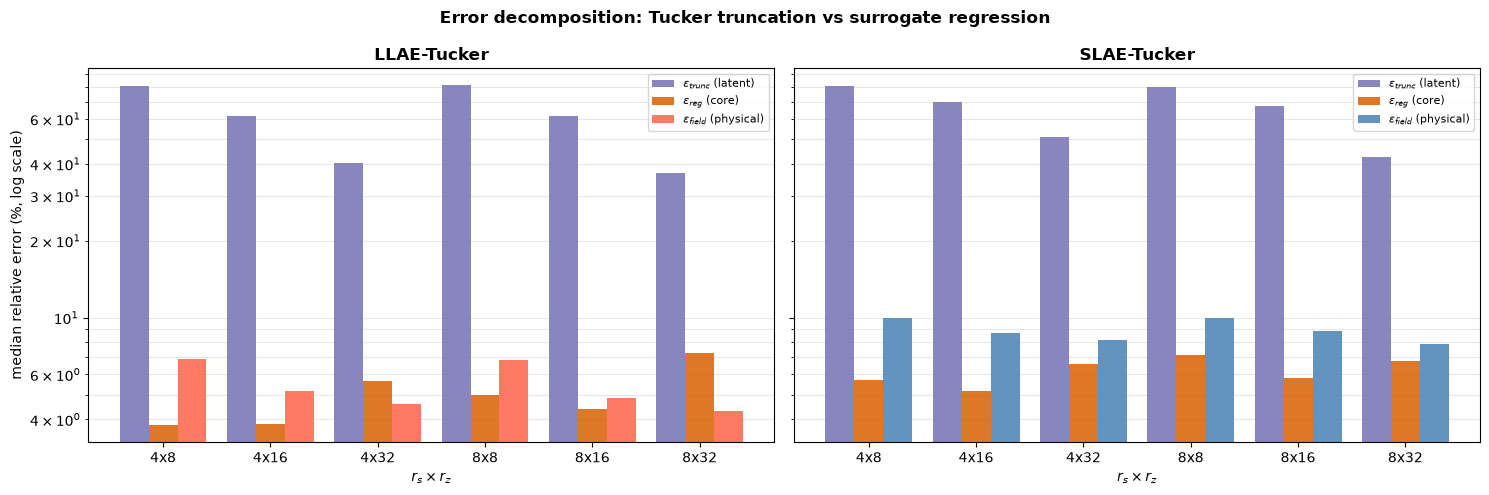
\includegraphics[width=\textwidth]{tucker_error_decomp.png}
    \caption{Error decomposition for LLAE-Tucker (left) and SLAE-Tucker (right): median latent truncation error $\varepsilon_{\mathrm{trunc}}$, core regression error $\varepsilon_{\mathrm{reg}}$, and physical-field error $\varepsilon_{\mathrm{field}}$ for each $(r_s, r_z)$ pair (log scale). The field error follows the truncation error, not the regression error.}
    \label{fig:tucker_error_decomp}
\end{figure}

\paragraph{Compression trade-off.}
Figure~\ref{fig:tucker_pareto} plots the field error against the compression ratio $\rho$ and against the surrogate size. Along the Pareto front, LLAE-Tucker degrades gracefully as the target is compressed: $r_s=4$, $r_z=32$ retains 4.57\% median error at $\rho = 0.125$ (an $8\times$ smaller target than the direct surrogate), and $r_s=4$, $r_z=16$ still reaches 5.16\% at $\rho = 0.062$ ($16\times$). Tucker therefore offers a tunable accuracy/compactness dial that the direct and SVD surrogates lack: when the surrogate output must be kept small — for storage, for a lightweight predictor, or for downstream many-query use — Tucker sustains near-direct accuracy at a fraction of the target dimension. It does not, however, \emph{beat} the direct surrogate on raw accuracy; as with SVD (Section~\ref{sec:ae_svd_surr}), reducing the latent space before the surrogate discards information the direct predictor is capable of learning.

\begin{figure}[htbp]
    \centering
    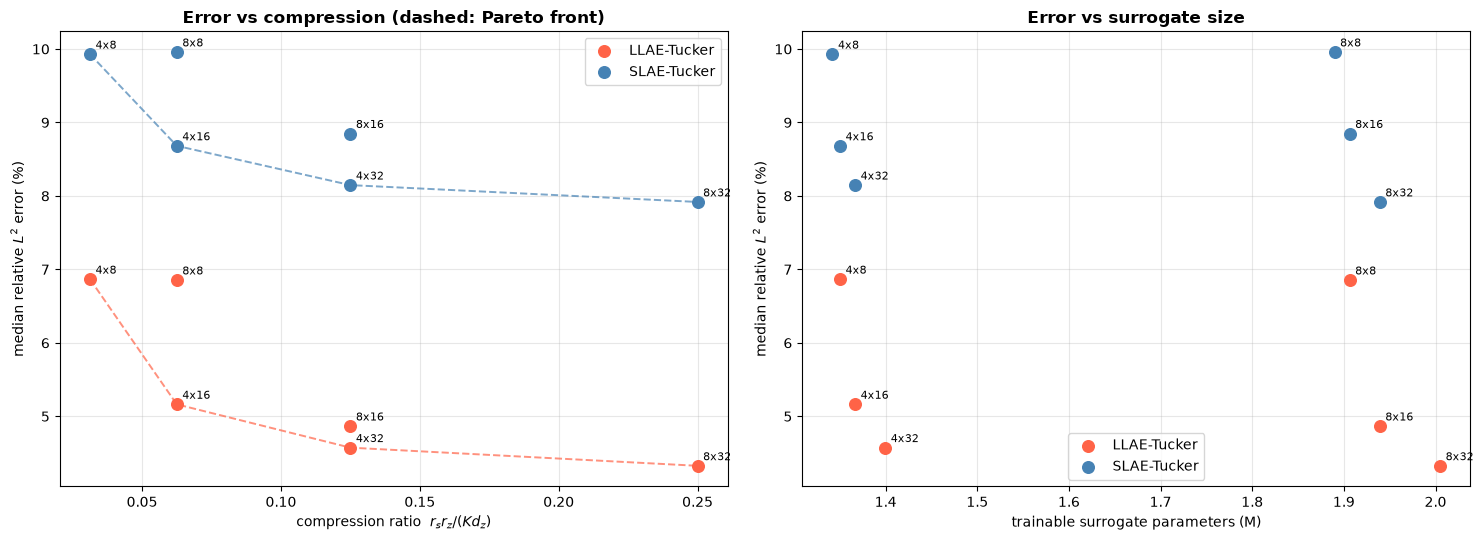
\includegraphics[width=\textwidth]{tucker_pareto.png}
    \caption{Left: median field error vs.\ compression ratio $\rho = r_s r_z / (K d_z)$ (dashed line = Pareto front per family; points sharing a ratio differ in $(r_s, r_z)$). Right: median field error vs.\ trainable surrogate parameters.}
    \label{fig:tucker_pareto}
\end{figure}

\paragraph{Decoder co-adaptation.}
A subtle consequence of the end-to-end fine-tuning (Section~\ref{sec:direct_surr}) is worth flagging. Because the decoder is jointly updated during surrogate training (\texttt{lr\_decoder}${=}5\times10^{-5}$), it can co-adapt to the distribution of \emph{predicted} cores rather than the true ones. We probe this by decoding the exact projected core in place of the surrogate's prediction: if the decoder had not co-adapted, the exact core would yield a lower error and serve as a valid oracle lower bound. For LLAE-Tucker the substitution is neutral ($+0.07$\,pp), so the oracle bound holds. For SLAE-Tucker, however, decoding the exact core \emph{raises} the error sharply ($+11.1$\,pp on the probe subsample at $r_s=8$, $r_z=16$): the SLAE decoder has specialised to the predicted-core distribution, exactly the mechanism that produced the negative surrogate Gap for SLAE in Section~\ref{sec:direct_surr}. A physical-space oracle is therefore not a valid lower bound for SLAE-Tucker, which is why the truncation and regression diagnostics above are computed in the latent space, where they remain decoder-independent.

\paragraph{Inference latency.}
The Tucker back-projection ($U^{(s)}\hat{\mathcal{G}}U^{(z)\top}$, two small matrix products) is negligible in the inference budget. Measured on an NVIDIA RTX A5000 at batch size 1 (Figure~\ref{fig:tucker_bench}), LLAE-Tucker runs at ${\sim}18$\,ms per sample and SLAE-Tucker at ${\sim}7$\,ms, essentially independent of the ranks and virtually identical to the direct and SVD pipelines. SLAE-Tucker thus preserves the ${\approx}2.4\times$ latency advantage of its lighter decoder, at the cost of the higher error floor discussed above.

\begin{figure}[htbp]
    \centering
    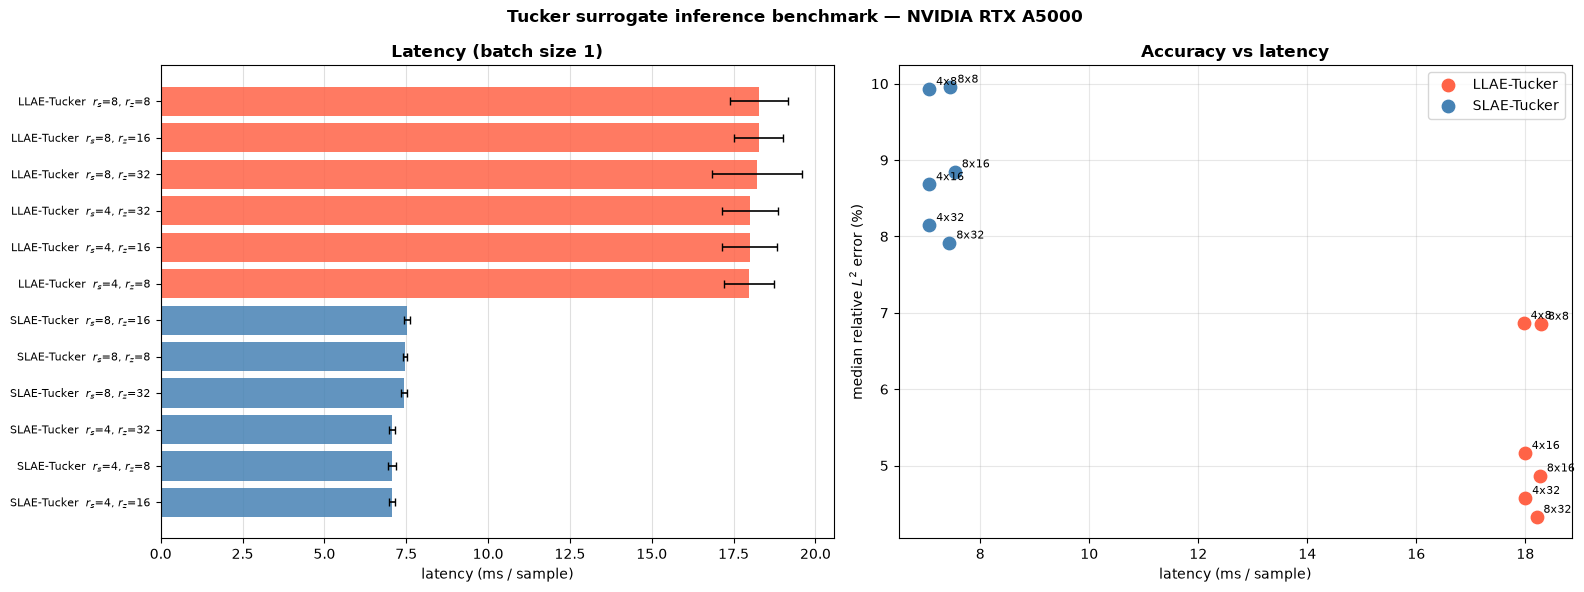
\includegraphics[width=\textwidth]{tucker_bench.png}
    \caption{Tucker surrogate inference benchmark (NVIDIA RTX A5000, 50 CUDA Event timed runs, batch size 1). Left: per-checkpoint latency. Right: accuracy--latency scatter. Latency is set by the decoder family, not the Tucker ranks.}
    \label{fig:tucker_bench}
\end{figure}

Per-checkpoint error histograms for all 12 Tucker surrogates are provided in Appendix~\ref{app:histograms} (Figure~\ref{fig:tucker_histograms}).

\subsection{Optimal laplace contour choice}

\section{Comparison and Discussion}
\subsection{Global synthesis}
\subsection{SLAE vs LLAE: a trade-off between speed and accuracy}

\subsection{Is latent compression worth it?}
\label{sec:compression_verdict}

Sections~\ref{sec:direct_surr}--\ref{sec:tucker_surr} evaluated three surrogate strategies — direct, single-mode SVD, and joint-mode Tucker — that differ only in how the latent prediction target is compressed. Do the compressed variants gain anything? On inference cost, the answer is no, and the reason is structural: the three pipelines share the same decoder, and it is the decoder — reconstructing the $K$ Laplace frames (SLAE) or all $N_t$ time frames (LLAE) — that dominates inference. SVD and Tucker change only the width of the MLP output head and insert a small linear back-projection ($V^\top$, or the two Tucker factors) before decoding; neither touches the decoder workload. Latency is therefore effectively invariant to the compression strategy: within each family the three pipelines fall in the same band ($\text{SLAE} \sim 7$--$9$\,ms, $\text{LLAE} \sim 18$--$22$\,ms at batch size~1 on the RTX A5000), the SVD variant being marginally the slowest because of its per-frequency back-projection. Table~\ref{tab:compression_verdict} places accuracy, target dimension and latency side by side at the shared AE configuration.

\begin{table}[htbp]
    \centering
    \small
    \renewcommand{\arraystretch}{1.3}
    \begin{tabular}{llccc}
        \toprule
        \textbf{Family} & \textbf{Strategy} & \textbf{Target (coeff.)} & \textbf{Median (\%)} & \textbf{Latency (ms)} \\
        \midrule
        \multirow{3}{*}{LLAE}
          & Direct                          & 1024 & 4.18 & 18.3 \\
          & SVD ($k_{\mathrm{svd}}=32$)              &  512 & 4.24 & ${\sim}22$ \\
          & Tucker ($r_s{=}8$, $r_z{=}32$)  &  256 & 4.33 & 18.2 \\
        \midrule
        \multirow{3}{*}{SLAE}
          & Direct                          & 1024 & 7.59 & 8.4 \\
          & SVD ($k_{\mathrm{svd}}=32$)              &  512 & 7.90 & ${\sim}9$ \\
          & Tucker ($r_s{=}8$, $r_z{=}32$)  &  256 & 7.92 & 7.4 \\
        \bottomrule
    \end{tabular}
    \caption{Direct vs.\ SVD vs.\ Tucker at the shared autoencoder configuration ($d_z=64$, $K=16$, $\gamma=0.01$). \emph{Target (coeff.)}: number of latent coefficients the surrogate predicts per sample ($K d_z$, $K k_{\mathrm{svd}}$, $r_s r_z$ respectively; complex-valued for LLAE, real for SLAE). Median relative $L^2$ error on the test set ($n=1620$); latency at batch size~1 on the NVIDIA RTX A5000. Compression shrinks the target by up to $4\times$ but leaves accuracy and latency essentially unchanged.}
    \label{tab:compression_verdict}
\end{table}

The verdict is clear. Relative to the direct surrogate, neither SVD nor Tucker improves accuracy (each adds a fraction of a point) nor latency (the pipeline is decoder-bound). What they \emph{do} buy is a smaller, simpler prediction target — Tucker down to $256$ coefficients, a $4\times$ reduction over the direct $K d_z = 1024$. That compactness only pays off when the surrogate, not the decoder, is the binding constraint: a tight training-data budget, storage or transmission of the predicted coefficients, or downstream analysis of the compact Tucker core. For the present problem, where the decoder governs both cost and error, the \emph{direct} surrogate is the pragmatic choice; the value of SVD and Tucker is chiefly methodological, showing that most of the latent's predictive content survives aggressive rank reduction.

\subsection{The importance of choosing an optimal Laplace contour}

\subsection{Positioning with respect to related work}
\label{sec:positioning}

Our pipeline reuses well-established components and combines them along a new axis. The \emph{spatial} compressor is a convolutional encoder--decoder applied directly to the field, i.e.\ the deep convolutional-autoencoder ROM of Lee and Carlberg~\cite{lee2020} and of the original DL-ROM~\cite{fresca2021}; we deliberately omit the preliminary POD reduction of POD-DL-ROM~\cite{fresca2022}, which is an efficiency device (it lowers the autoencoder's training cost) rather than an accuracy device, and is unnecessary for a convolutional network operating on a structured grid. The \emph{linear} baseline against which we measure the nonlinear gain is a POD basis followed by a parameter-to-coefficient network, that is, the non-intrusive POD-NN of Hesthaven and Ubbiali~\cite{hesthaven2018}, here applied frequency-by-frequency in the Laplace domain. Our optional SVD and Tucker stages (Sections~\ref{sec:svd_compression}--\ref{sec:tucker_compression}) also use linear/multilinear projections, but in a role opposite to POD-DL-ROM: they act \emph{after} the nonlinear autoencoder, in the latent space, to shrink the surrogate target — a post-compression, not a spatial pre-reduction.

What distinguishes our approach is not the spatial compressor but the treatment of \emph{time}. All the DL-ROMs above keep the full temporal resolution of the trajectory: the reduced dynamics are queried once per time step through a $(\vmu, t)$-conditioned network~\cite{fresca2021,fresca2022} or propagated sequentially in time~\cite{pant2021deep}, so the temporal work scales with $N_t$. We instead compress the time axis itself with the Laplace transform, predicting $K \ll N_t$ spectral coefficients in a single shot and recovering the full trajectory by a cheap linear inversion. This exploits the same spectral intuition as Laplace-domain linear ROMs~\cite{reyes2025,goeckner2022} and the Laplace Neural Operator~\cite{cao2023}, but transposes it into the \emph{nonlinear}, \emph{parameter-to-field} DL-ROM setting, where — to our knowledge — temporal Laplace compression has not previously been used. The Laplace stage is therefore orthogonal to the spatial-compression choices above and could in principle be layered on top of any of them, including POD-DL-ROM.

\paragraph{Relation to neural operators.} The learnable-contour variant of LLAE (Section~\ref{sec:contour_optim}) deserves a closer comparison with operator-learning methods, which it resembles along two axes. First, it applies its spectral transform \emph{inside a learned low-dimensional latent space} rather than on the physical field, exactly the design principle of the Latent Neural Operator~\cite{wang2024lno}: encode to a compact latent, act there, decode back. Second, and more specifically, learning the complex poles $s_k = \sigma_k + i\omega_k$ end-to-end is a latent-space counterpart of the learnable pole--residue representation at the heart of the Laplace Neural Operator~\cite{cao2023}; in both cases the temporal (or trajectory) dynamics are captured by a small set of trainable poles in the complex plane rather than by a fixed spectral grid or by explicit time-stepping. The surrogate itself reinforces the analogy: its shared trunk conditioned on a sinusoidal encoding of the frequency $s_k$ (Figure~\ref{fig:freq_surrogate_arch}) maps $(\vmu, s_k) \mapsto \hat{z}(s_k)$, so the Laplace frequency plays the role of the output coordinate much as the trunk coordinate does in a DeepONet~\cite{lu2021deeponet}. The essential difference is one of \emph{setting}, not of mechanism: genuine neural operators are field-to-field maps between function spaces, discretization-invariant in their input, whereas our input is a finite parameter vector $\vmu$ and our spatial decoder is a fixed-resolution convolutional network. LLAE with a learnable contour is thus best understood as a \emph{parameter-conditioned, latent Laplace operator} — importing the learnable-pole and latent-operator ideas from~\cite{cao2023,wang2024lno} into the DL-ROM regime, rather than as a neural operator in the strict field-to-field sense.

\subsection{Discussion and perspectives}


\newpage
\begin{appendices}
\addtocontents{toc}{\protect\setcounter{tocdepth}{0}}

\clearpage
\section{Per-Checkpoint Error Distributions}
\label{app:histograms}

\paragraph{POD reconstruction.} Figure~\ref{fig:pod_rec_histograms} shows the distribution of relative $L^2$ errors for each of the 7 POD reconstruction configurations evaluated in Section~\ref{sec:pod_results}.

\begin{figure}[htbp]
    \centering
    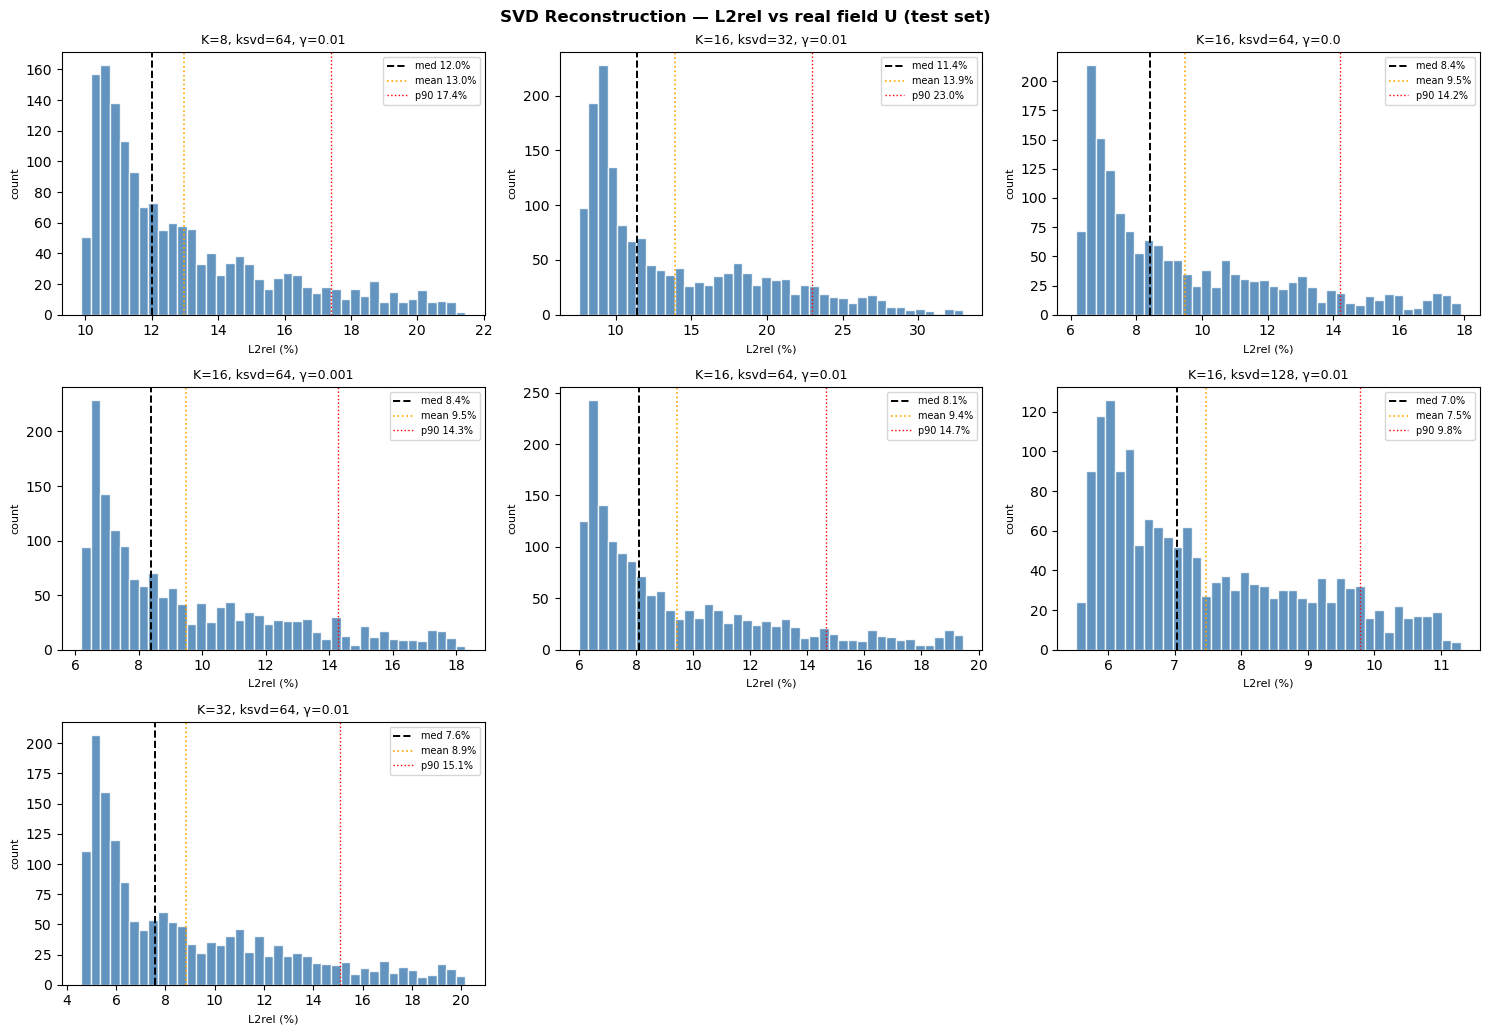
\includegraphics[width=\textwidth]{svd_rec_histograms.png}
    \caption{Per-configuration error histograms for the POD reconstruction (test set, $n=1620$). The dashed black line is the median, dashed orange the mean, dotted red the 90th percentile.}
    \label{fig:pod_rec_histograms}
\end{figure}

\paragraph{POD surrogate.} Figure~\ref{fig:pod_surr_histograms} shows the corresponding distributions for the end-to-end POD surrogate (Section~\ref{sec:pod_results}).

\begin{figure}[htbp]
    \centering
    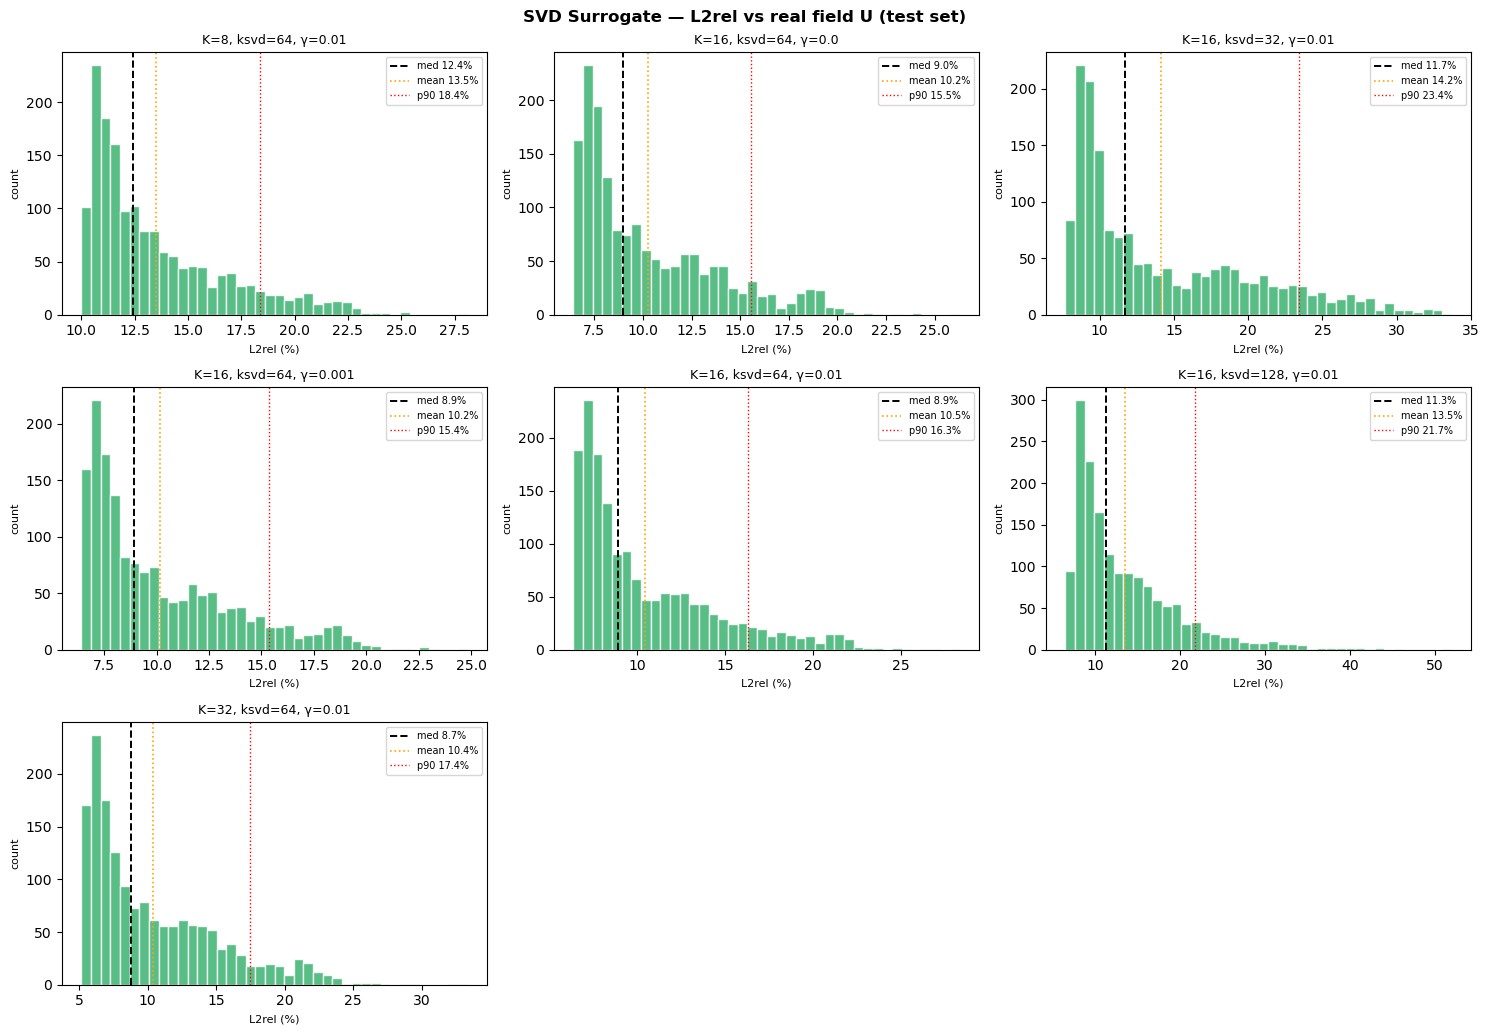
\includegraphics[width=\textwidth]{svd_surr_histograms.png}
    \caption{Per-configuration error histograms for the POD surrogate (test set, $n=1620$). Same layout as Figure~\ref{fig:pod_rec_histograms}; green bars indicate surrogate predictions.}
    \label{fig:pod_surr_histograms}
\end{figure}

\paragraph{AE checkpoints.} Figure~\ref{fig:ae_histograms} shows the distribution of relative $L^2$ errors across the 1620 test simulations for each of the 14 AE checkpoints evaluated in Section~\ref{sec:ae_perf}. Dashed lines indicate the median (black) and mean (orange); the dotted red line marks the 90th percentile.

\begin{figure}[htbp]
    \centering
    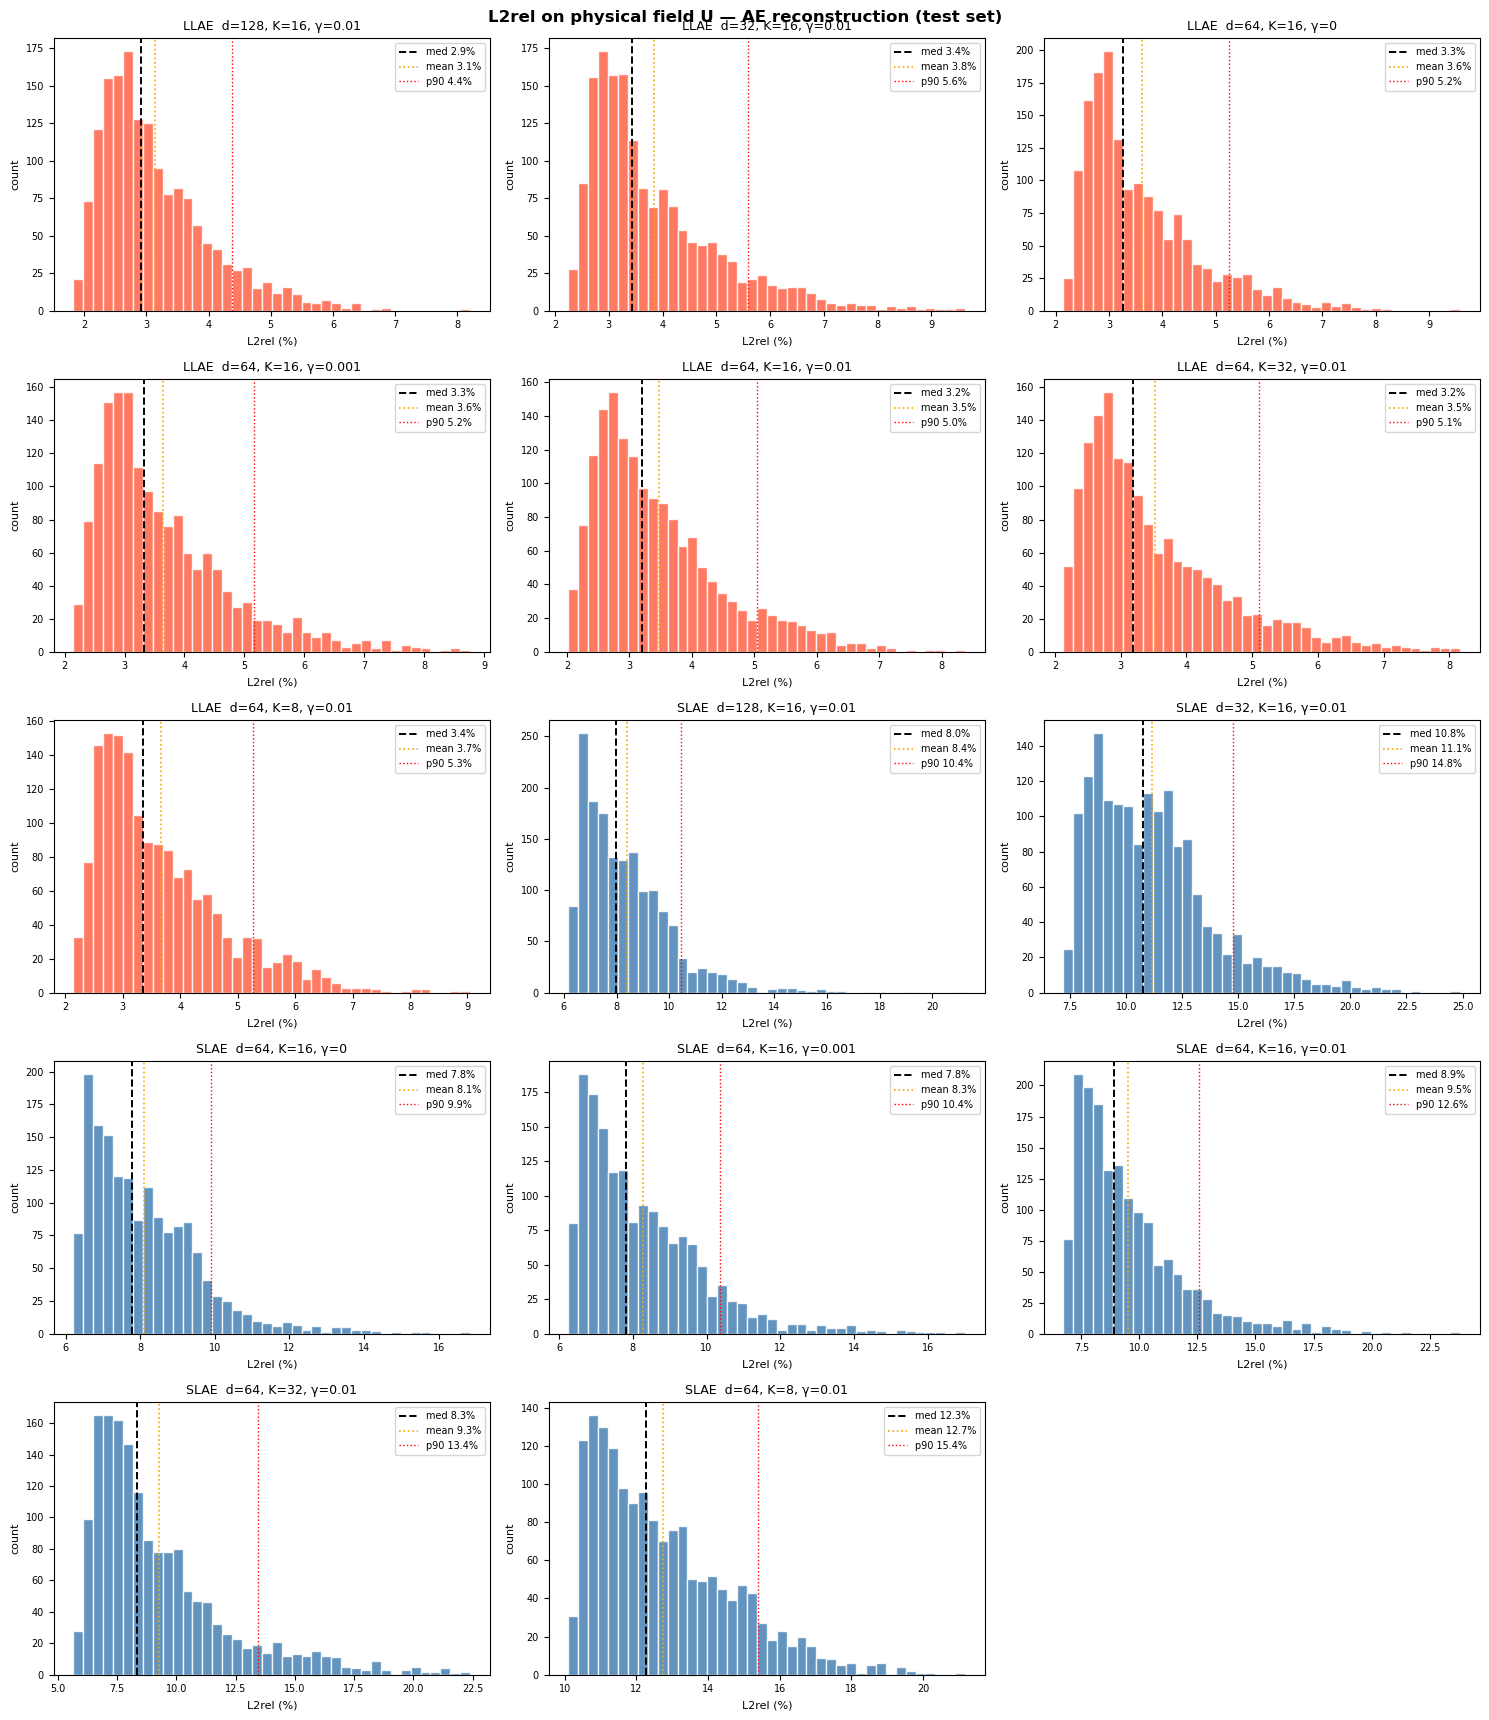
\includegraphics[width=\textwidth]{ae_histograms_all.png}
    \caption{Per-checkpoint error histograms on the test set ($n=1620$). Each panel corresponds to one checkpoint; SLAE in blue, LLAE in red. The dashed black line is the median, dashed orange the mean, dotted red the 90th percentile.}
    \label{fig:ae_histograms}
\end{figure}

\paragraph{Surrogate checkpoints.}
Figure~\ref{fig:surr_histograms} shows the per-sample error distribution for each of the 14 direct surrogate checkpoints evaluated in Section~\ref{sec:direct_surr}.

\begin{figure}[htbp]
    \centering
    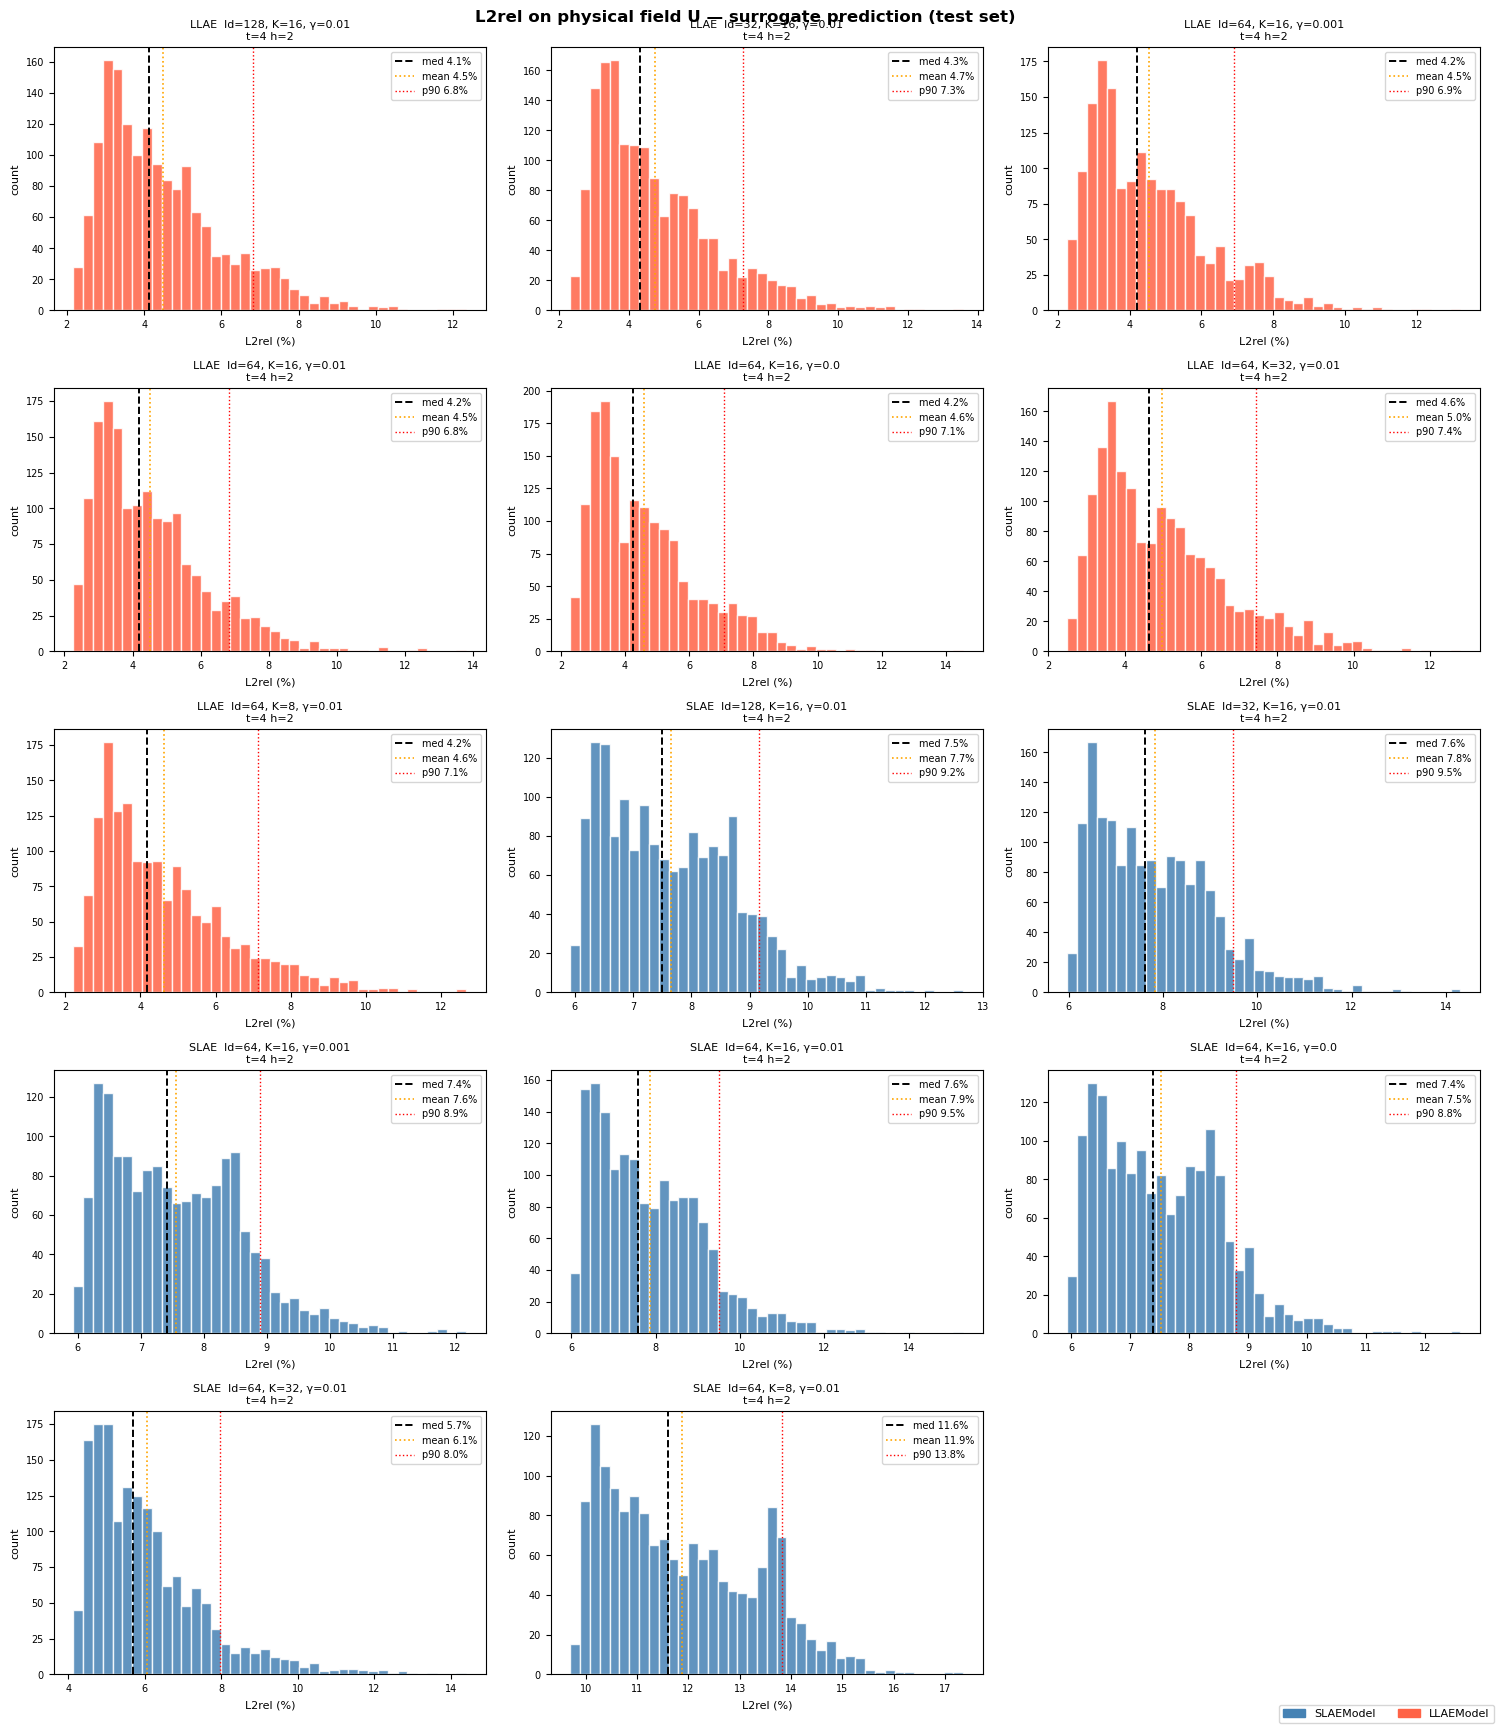
\includegraphics[width=\textwidth]{surr_histograms.png}
    \caption{Per-checkpoint error histograms for all 14 direct surrogate models (test set, $n=1620$). SLAE checkpoints in blue, LLAE checkpoints in red. The dashed black line is the median, dashed orange the mean, dotted red the 90th percentile.}
    \label{fig:surr_histograms}
\end{figure}

\paragraph{Tucker surrogate checkpoints.}
Figure~\ref{fig:tucker_histograms} shows the per-sample error distribution for each of the 12 Tucker surrogate checkpoints evaluated in Section~\ref{sec:tucker_surr}.

\begin{figure}[htbp]
    \centering
    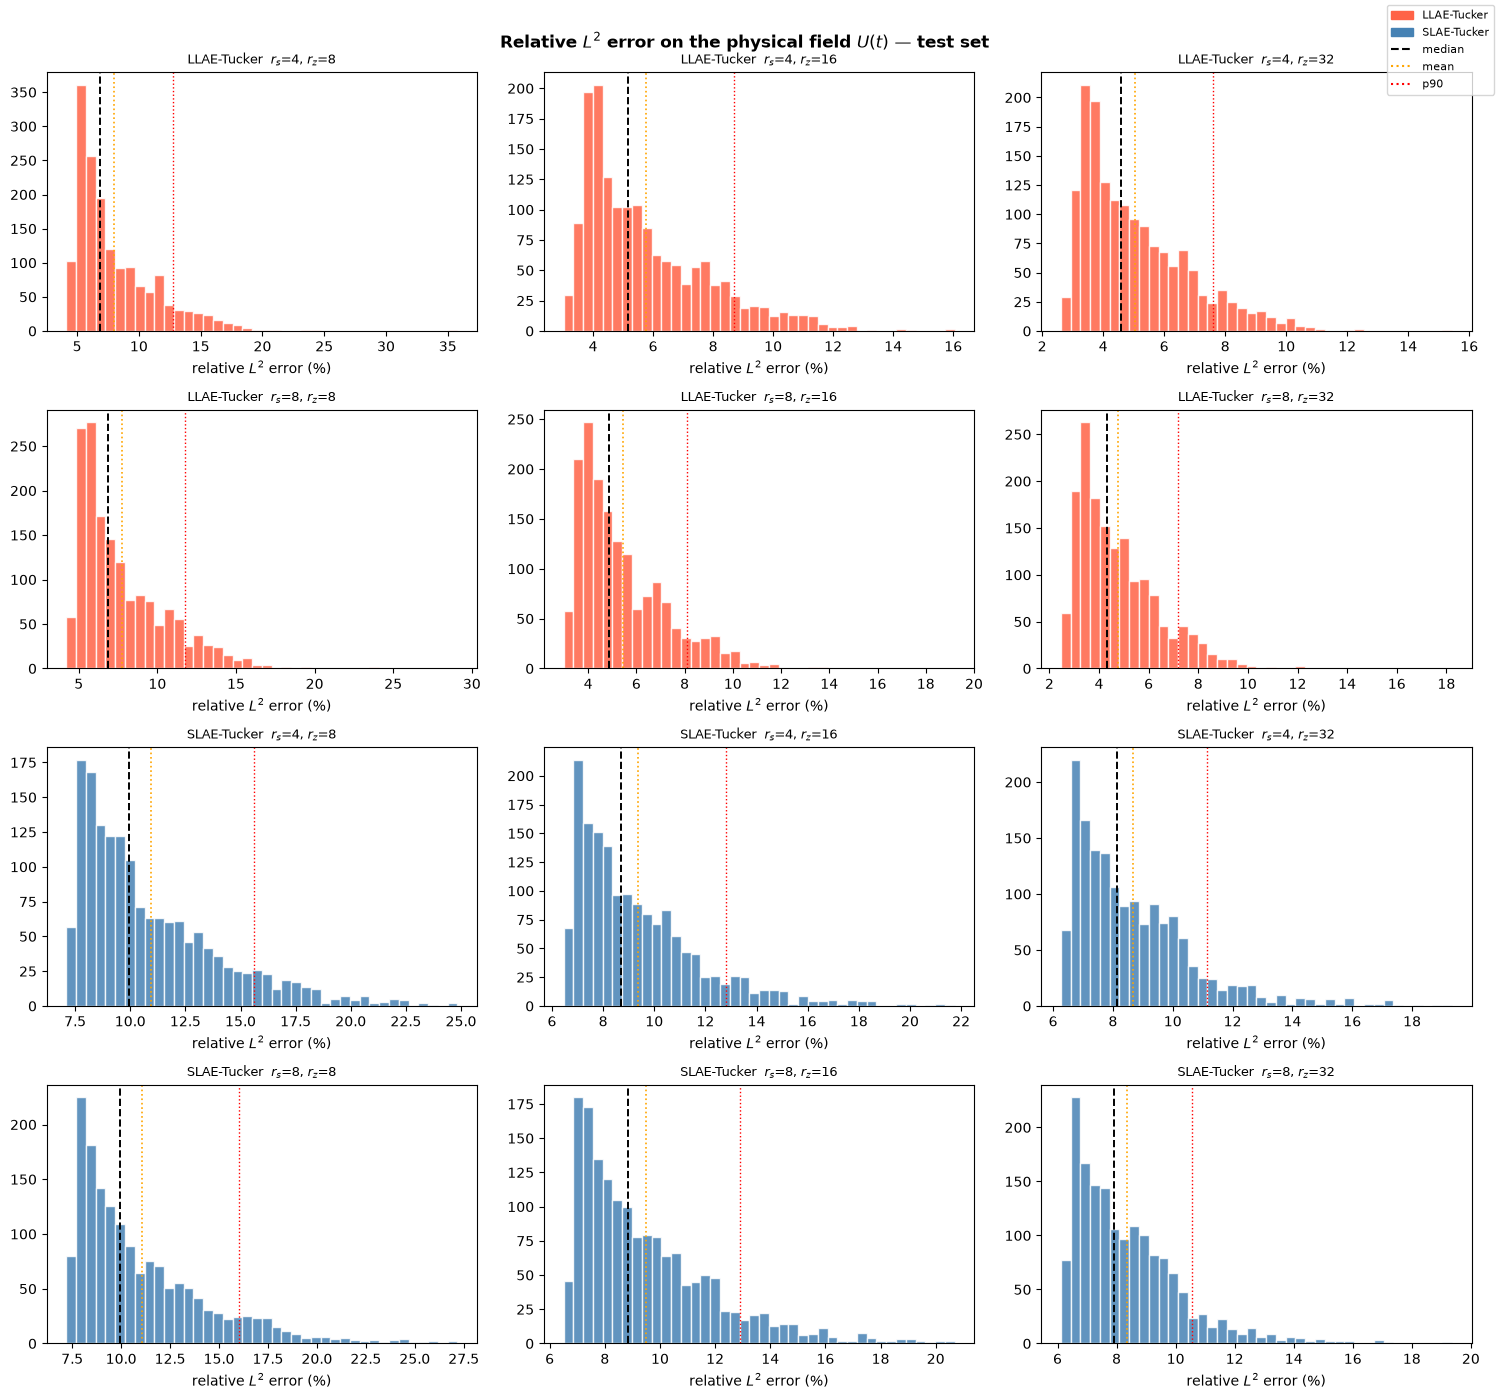
\includegraphics[width=\textwidth]{tucker_histograms.png}
    \caption{Per-checkpoint error histograms for all 12 Tucker surrogate models (test set, $n=1620$). SLAE-Tucker in blue, LLAE-Tucker in red. The dashed black line is the median, dashed orange the mean, dotted red the 90th percentile.}
    \label{fig:tucker_histograms}
\end{figure}

\clearpage
\section{POD Baseline: Full Ablations}
\label{app:pod_ablation}

This appendix collects the complete hyperparameter sweeps behind Section~\ref{sec:pod_results}, for both the pure POD reconstruction and the end-to-end POD surrogate.

\begin{figure}[htbp]
    \centering
    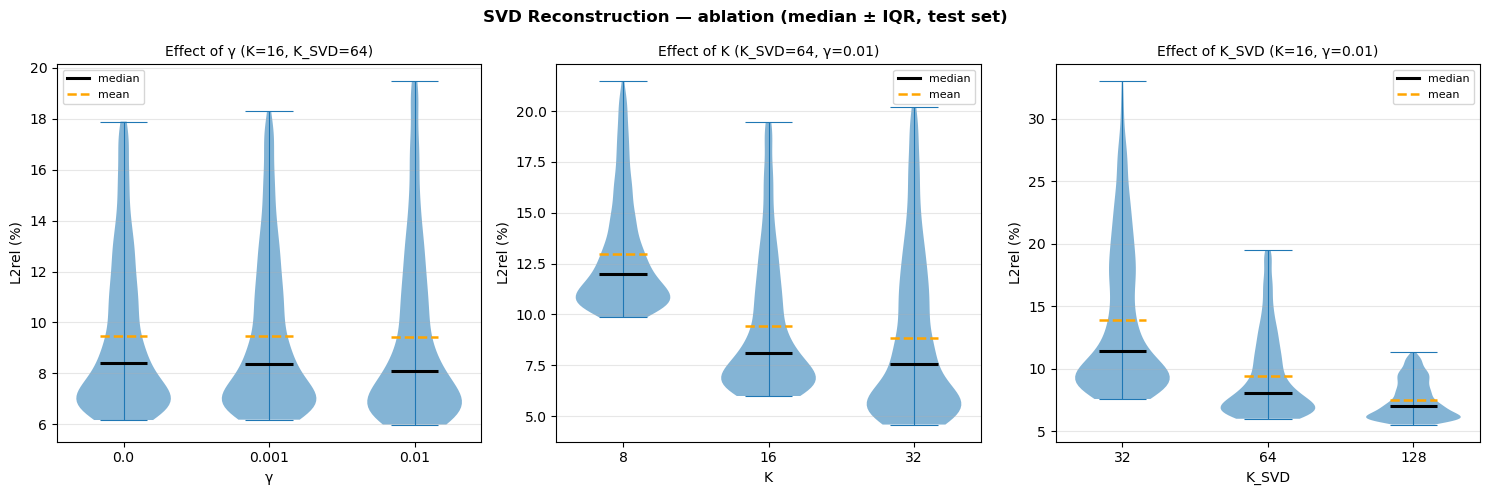
\includegraphics[width=\textwidth]{svd_rec_ablation.png}
    \caption{POD reconstruction ablation (test set, median $\pm$ IQR, violin plots; black line = median, dashed orange = mean). From left to right: effect of the damping parameter $\gamma$ ($K=16$, $k_{\mathrm{pod}}=64$), effect of the number of Laplace frequencies $K$ ($k_{\mathrm{pod}}=64$, $\gamma=0.01$), and effect of the number of POD modes $k_{\mathrm{pod}}$ ($K=16$, $\gamma=0.01$).}
    \label{fig:pod_ablation}
\end{figure}

\begin{figure}[htbp]
    \centering
    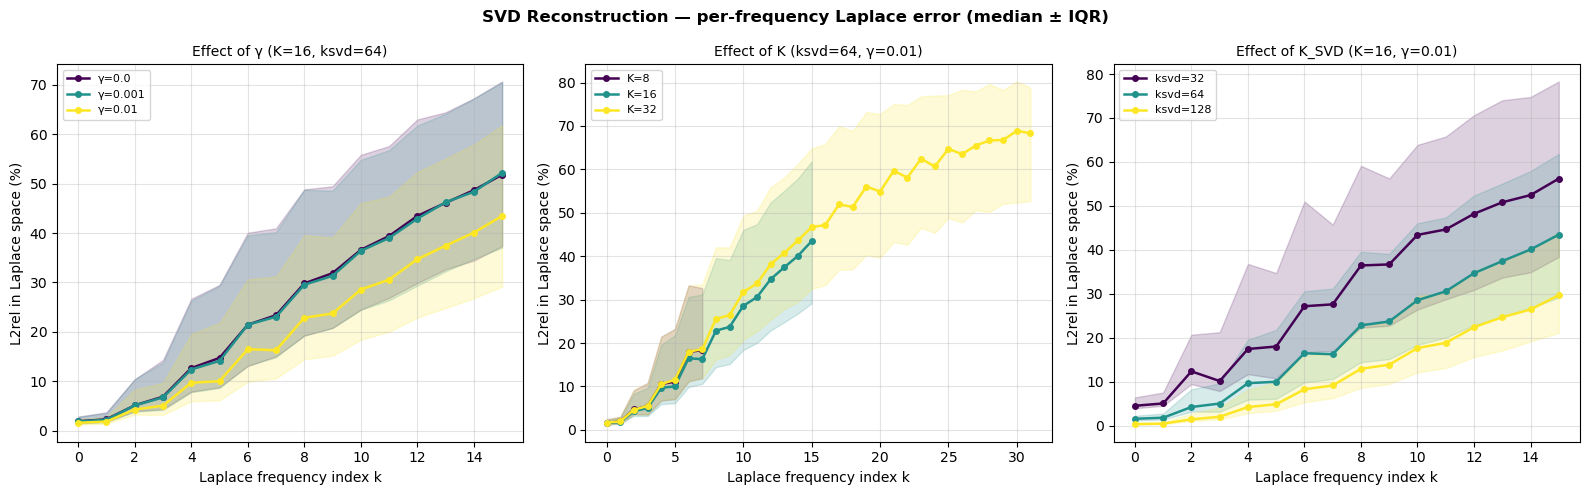
\includegraphics[width=\textwidth]{svd_rec_per_freq.png}
    \caption{POD reconstruction — per-frequency Laplace-domain error (median $\pm$ IQR, test set). Left: effect of $\gamma$; centre: effect of $K$; right: effect of $k_{\mathrm{pod}}$. The left panel exposes the trade-off discussed in Section~\ref{sec:pod_results}: the Laplace-domain error is systematically \emph{lower} for $\gamma=0$ at every frequency index, yet the net physical-field error is nearly unchanged, because the Tikhonov inversion error moves in the opposite direction.}
    \label{fig:pod_per_freq}
\end{figure}

\begin{figure}[htbp]
    \centering
    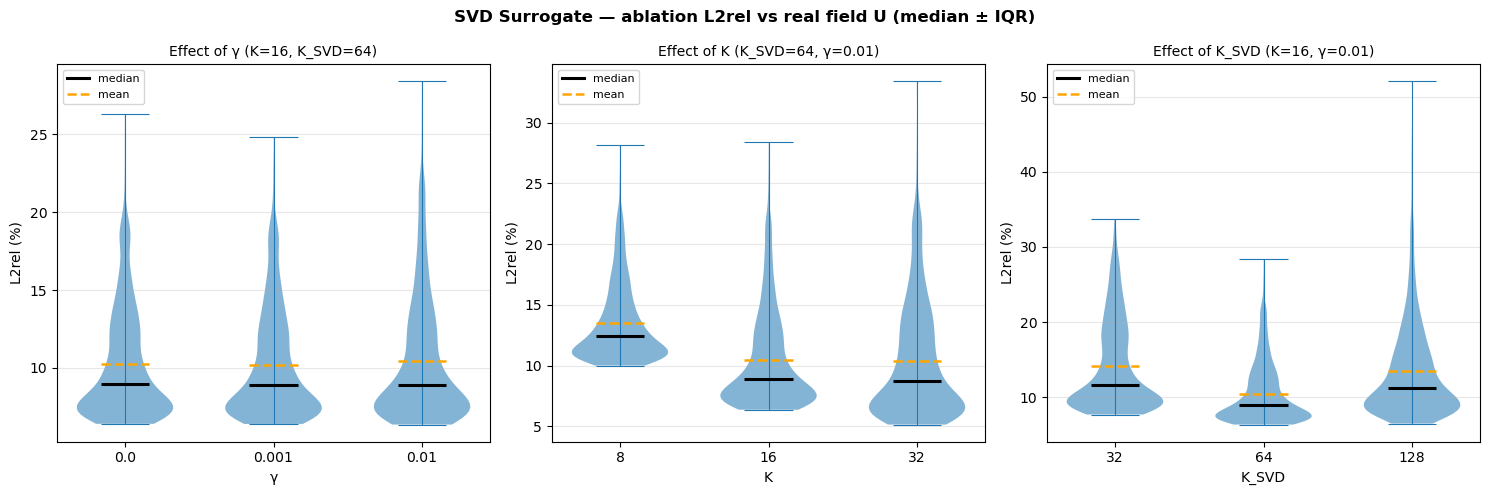
\includegraphics[width=\textwidth]{svd_surr_ablation.png}
    \caption{POD surrogate ablation (test set, median $\pm$ IQR). From left to right: effect of $\gamma$ ($K=16$, $k_{\mathrm{pod}}=64$), effect of $K$ ($k_{\mathrm{pod}}=64$, $\gamma=0.01$), and effect of $k_{\mathrm{pod}}$ ($K=16$, $\gamma=0.01$). Black line = median, dashed orange = mean.}
    \label{fig:svd_surr_ablation}
\end{figure}

\begin{figure}[htbp]
    \centering
    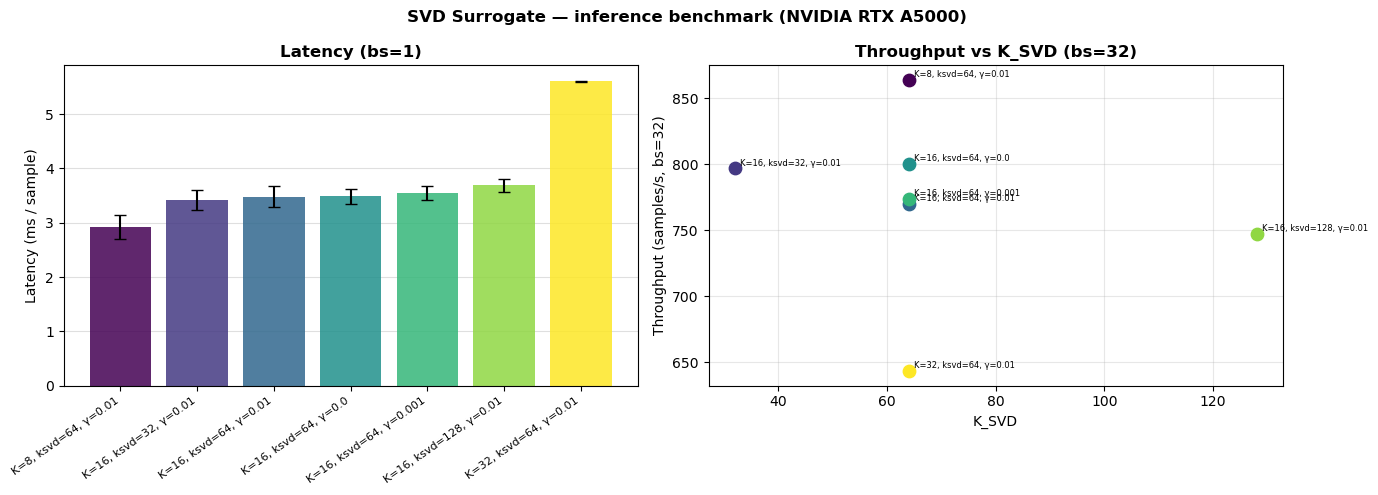
\includegraphics[width=\textwidth]{svd_surr_bench.png}
    \caption{POD surrogate inference benchmark (NVIDIA RTX A5000, 50 timed CUDA Event runs, 10 warm-up runs). Left: per-sample latency at batch size 1, sorted by latency. Right: throughput (samples/s) vs.\ $k_{\mathrm{pod}}$ at batch size 32.}
    \label{fig:pod_surr_bench}
\end{figure}

\clearpage
\section{Surrogate Ablation Studies}
\label{app:surr_ablation}

Figures~\ref{fig:llae_surr_ablation} and~\ref{fig:slae_surr_ablation} show the effect of each hyperparameter on the end-to-end surrogate error, using violin plots of the full test-set distribution (one hyperparameter varied at a time, others fixed at the baseline values of Table~\ref{tab:ae_hparams}).

\begin{figure}[htbp]
    \centering
    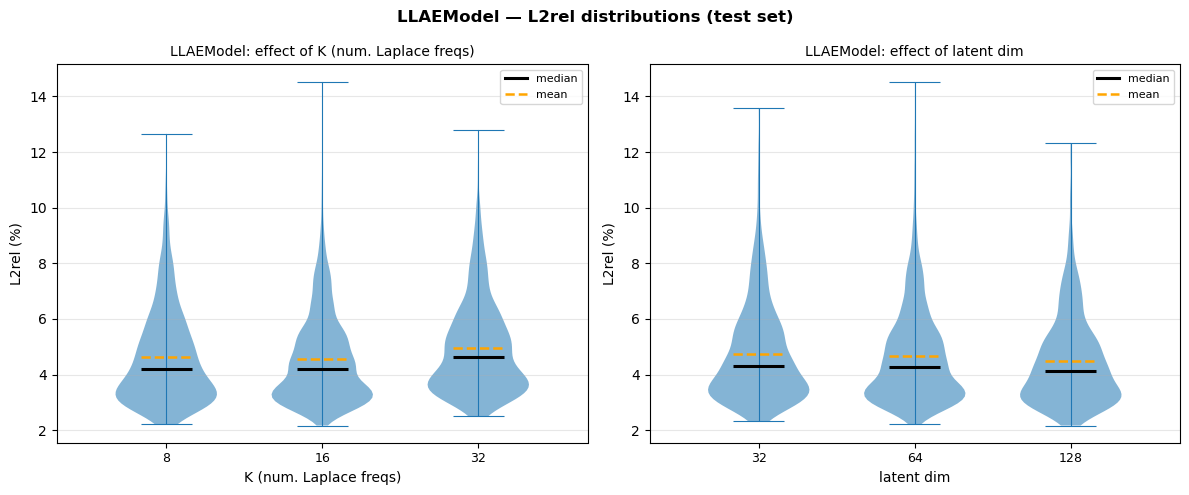
\includegraphics[width=\textwidth]{llae_surr_ablation.png}
    \caption{LLAE surrogate ablation (test set, $n=1620$, violin plots; black line = median, dashed orange = mean). From left to right: effect of the number of Laplace frequencies $K$ ($d_z=64$, $\gamma=0.01$) and effect of the latent dimension $d_z$ ($K=16$, $\gamma=0.01$). The surrogate error varies by less than 0.5\,pp across all LLAE configurations.}
    \label{fig:llae_surr_ablation}
\end{figure}

\begin{figure}[htbp]
    \centering
    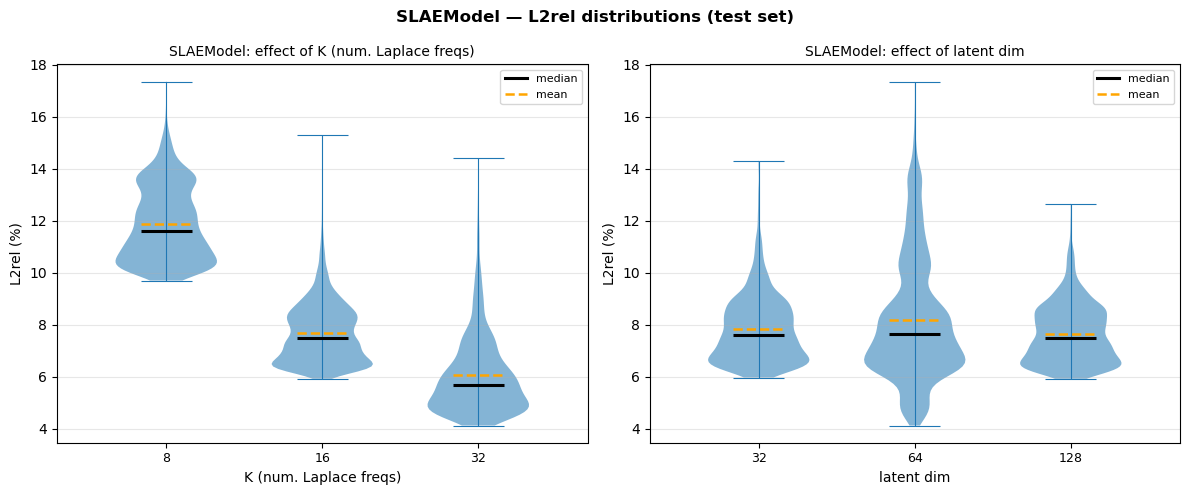
\includegraphics[width=\textwidth]{slae_surr_ablation.png}
    \caption{SLAE surrogate ablation (test set, $n=1620$). Same layout as Figure~\ref{fig:llae_surr_ablation}. SLAE error is strongly sensitive to $K$: $K=8$ degrades to 11.6\% while $K=32$ achieves the best SLAE result (5.7\%). Note the larger $y$-axis range compared to LLAE.}
    \label{fig:slae_surr_ablation}
\end{figure}

\clearpage
\section{Governing Equations}
\label{app:equations}

Our neural surrogate model is designed to emulate the transient dynamics of a reacting flow system. The physical system is governed by a set of coupled partial differential equations representing the conservation of mass, momentum, energy, and chemical species.

\begin{enumerate}
    \item \textbf{Fluid Mechanics (Momentum):}
    \begin{equation}
        \frac{\partial(\rho\mathbf{U})}{\partial t} + \nabla \cdot (\rho\mathbf{U}\mathbf{U}) - \nabla \cdot \tau = -\nabla p + \rho\mathbf{g}
    \end{equation}

    \item \textbf{Chemical Species Transport:}
    \begin{equation}
        \frac{\partial(\rho Y_i)}{\partial t} + \nabla \cdot (\rho\mathbf{U}Y_i) - \nabla \cdot (\mu_{\mathrm{eff}}\nabla Y_i) = \dot{\omega}_{i,\mathrm{eff}}
    \end{equation}
    under the constraint $\sum Y_i = 1$.

    \item \textbf{Energy:}
    \begin{equation}
        \frac{\partial(\rho h)}{\partial t} + \nabla \cdot (\rho\mathbf{U}h) + \frac{\partial(\rho K)}{\partial t} + \nabla \cdot (\rho\mathbf{U}K) - \frac{\partial p}{\partial t} - \nabla \cdot (\alpha_{\mathrm{eff}}\nabla h) = \dot{q}_{\mathrm{chem}}
    \end{equation}
    where $K = \frac{1}{2}|\mathbf{U}|^2$ is the kinetic energy.

    \item \textbf{Combustion Model (PaSR):}
    The effective reaction rate is modulated by the Partially Stirred Reactor model:
    \begin{equation}
        \dot{\omega}_{i,\mathrm{eff}} = \kappa\dot{\omega}_i(c^*, T^*), \quad \text{with} \quad \kappa = \frac{\tau_c}{\tau_c + \tau_{\mathrm{mix}}}
    \end{equation}
    where $\tau_c$ and $\tau_{\mathrm{mix}}$ are the characteristic chemical and turbulent mixing times, respectively.

    \item \textbf{Equation of State:}
    The ideal gas law closes the system:
    \begin{equation}
        p = \rho R T \quad \text{or} \quad \rho = \psi p \quad \text{with} \quad \psi = \frac{1}{R T}
    \end{equation}
\end{enumerate}

\clearpage
\section{Architectural Details and Setup}
\label{app:architecture}

All models were trained using the AdamW optimizer (weight decay $10^{-4}$) with a learning rate of $5 \times 10^{-4}$ for the autoencoders, $3 \times 10^{-4}$ for the surrogate trunk, and $5 \times 10^{-5}$ for the fine-tuned decoder, over 300 epochs. The autoencoders used a batch size of 256 (SLAE) or 16 (LLAE). Training was performed on a workstation equipped with an Intel(R) Xeon(R) w3-2435 CPU (62GB RAM) and an NVIDIA GeForce RTX 3090 GPU (24GB VRAM). Training data consists of 6480 simulations; the test set contains 1620 samples.

Table~\ref{tab:ae_hparams} summarises the hyperparameters of both autoencoder architectures.

\begin{table}[H]
    \centering
    \renewcommand{\arraystretch}{1.3}
    \begin{tabular}{llcc}
        \toprule
        \textbf{Group} & \textbf{Hyperparameter} & \textbf{SLAE} & \textbf{LLAE} \\
        \midrule
        \multirow{4}{*}{Architecture (baseline$^\dagger$)}
          & Latent dim $d_z$           & 64   & 64   \\
          & Frequencies $K$            & 16   & 16   \\
          & Sinusoidal levels $L$      & 8    & 8    \\
          & Contour $\gamma$           & 0.01 & 0.01 \\
        \midrule
        \multirow{4}{*}{Regularization}
          & Ridge $\beta$              & $10^{-2}$ & $10^{-2}$ \\
          & Latent roundtrip $\beta_\text{latent}$ & --- & $0.1$ \\
          & Tikhonov $\alpha_t$        & $7\times10^{-3}$ (eval) & $7\times10^{-3}$ \\
          & Tikhonov $\lambda$         & $3\times10^{-5}$ (eval) & $3\times10^{-5}$ \\
        \midrule
        \multirow{4}{*}{Training}
          & Epochs                     & 300  & 300  \\
          & Batch size                 & 256   & 16   \\
          & Learning rate              & $5\times10^{-4}$ & $5\times10^{-4}$ \\
          & Early stopping patience    & 40   & 40   \\
        \bottomrule
    \end{tabular}
    \caption{Autoencoder hyperparameters. $^\dagger$Baseline values fixed when the other architectural parameters are swept: $d_z \in \{32, 64, 128\}$, $K \in \{8, 16, 32\}$, $\gamma \in \{0.0, 0.001, 0.01\}$.}
    \label{tab:ae_hparams}
\end{table}

Table~\ref{tab:surr_hparams} summarises the hyperparameters used for surrogate training (Phase 2).

\begin{table}[htbp]
    \centering
    \renewcommand{\arraystretch}{1.3}
    \begin{tabular}{llcc}
        \toprule
        \textbf{Group} & \textbf{Hyperparameter} & \textbf{SLAE} & \textbf{LLAE} \\
        \midrule
        \multirow{4}{*}{Architecture (fixed)}
          & Trunk layers $n_\text{trunk}$  & 4   & 4   \\
          & Trunk hidden dim               & 512 & 512 \\
          & Head layers $n_\text{head}$    & 2   & 2   \\
          & Head hidden dim                & 256 & 256 \\
        \midrule
        \multirow{4}{*}{Loss}
          & Latent weight $\alpha_\text{lat}$  & 1.0 & 1.0 \\
          & Spatial weight $\alpha_\text{spat}$ & 1.0 & 1.0 \\
          & Tikhonov $\alpha_t$                & $7\times10^{-3}$ & $7\times10^{-3}$ \\
          & Tikhonov $\lambda$                 & $3\times10^{-5}$ & $3\times10^{-5}$ \\
        \midrule
        \multirow{6}{*}{Training}
          & Epochs                        & 300  & 300  \\
          & Batch size                    & 256  & 16   \\
          & $lr_\text{surrogate}$         & $3\times10^{-4}$ & $3\times10^{-4}$ \\
          & $lr_\text{decoder}$           & $5\times10^{-5}$ & $5\times10^{-5}$ \\
          & Weight decay                  & $10^{-4}$ & $10^{-4}$ \\
          & Early stopping patience       & 40   & 40   \\
        \bottomrule
    \end{tabular}
    \caption{Surrogate training hyperparameters (Phase 2). MLP architecture and training setup are fixed across all runs; one surrogate is trained per AE checkpoint (14 total, sweeping $d_z$, $K$, $\gamma$ as in Table~\ref{tab:ae_hparams}). The AE decoder is fine-tuned at $lr_\text{decoder}$ while the surrogate MLP is trained at $lr_\text{surrogate}$.}
    \label{tab:surr_hparams}
\end{table}



\clearpage
\section{Proofs for the Bias--Variance Contour Optimization}
\label{app:bv_proof}

\begin{proposition}[Invertibility of $\bm{A}$]
Since $\lambda > 0$ and $\bm{D}_t^T\bm{D}_t$ is positive semi-definite, $\bm{L}_{\mathrm{reg}} = \alpha_t\bm{D}_t^T\bm{D}_t + \lambda\bm{I}$ is positive definite ($\bm{L}_{\mathrm{reg}} \succeq \lambda\bm{I}$). Thus $\bm{A} = \Re(\bm{F}^H\bm{F}) + \bm{L}_{\mathrm{reg}}$ is symmetric positive definite and hence invertible. The unique reconstructed solution is $\bm{u}^*(\vmu) = \bm{A}^{-1}\Re(\bm{F}^H\hat{\bm{u}}(\vmu))$.
\end{proposition}

\textit{Proof of Theorem~\ref{thm:bv}.}
Starting from decomposition \eqref{eq:bv_decomp} and applying the triangle inequality:
\[
    \|\bm{u}(\vmu) - \bm{u}_{\mathrm{rec}}(\vmu)\| \leq \|\bm{u}(\vmu) - \bm{u}^*(\vmu)\| + \|\bm{u}^*(\vmu) - \bm{u}_{\mathrm{rec}}(\vmu)\|.
\]
The first term equals $\|\bm{A}^{-1}\bm{L}_{\mathrm{reg}}\bm{u}(\vmu)\|$ by \eqref{eq:bias_simplified}. For the second term:
\[
    \bm{u}^*(\vmu) - \bm{u}_{\mathrm{rec}}(\vmu)
    = \bm{A}^{-1}\Re\!\left(\bm{F}^H\!\left(\hat{\bm{u}}(\vmu) - \tilde{\bm{u}}(\vmu)\right)\right).
\]
Applying sub-multiplicativity of the operator norm and $\|\Re(M)\| \leq \|M\|$ yields:
\[
    \|\bm{u}^*(\vmu) - \bm{u}_{\mathrm{rec}}(\vmu)\|
    \leq \|\bm{A}^{-1}\bm{F}^H\| \cdot \|\hat{\bm{u}}(\vmu) - \tilde{\bm{u}}(\vmu)\|_{\C^K},
\]
which gives \eqref{eq:bv_bound}. \hfill$\square$

\textit{Proof} ($\epsilon_{\mathrm{AE}}(s_k) \leq \mathcal{E}_{\mathrm{SVD}}(s_k)$).
A linear autoencoder with bottleneck dimension $d_z$ minimizing the mean squared reconstruction error recovers exactly the truncated SVD projection~\cite{baldi1989}. Since a nonlinear autoencoder with the same bottleneck dimension optimizes over a strictly larger class of functions (which includes all linear encoder--decoder pairs), its minimum reconstruction error satisfies $\epsilon_{\mathrm{AE}}(s_k) \leq \mathcal{E}_{\mathrm{SVD}}(s_k)$, as empirically confirmed in~\cite{wang2016autoencoder}. \hfill$\square$

\end{appendices}

\bibliographystyle{plain}
\bibliography{refs}

\end{document}